\clearpage
\section{M-QAM Transmission System}

% Show subsubsections on the Table of Contents
\setcounter{tocdepth}{3}		
\setcounter{secnumdepth}{3}

\begin{refsection}

\begin{tcolorbox}
	\begin{tabular}{p{2.75cm} p{0.2cm} p{10.5cm}}
		\textbf{Student Name}  & & Andoni Santos (2018/01/03 - )\\
							   & & Ana Luisa Carvalho (2017/04/01 - 2017/12/31) \\
		\textbf{Goal}          &:& M-QAM system implementation with BER measurement and comparison with theoretical and experimental values.\\
		\textbf{Directory} &:& sdf/m\_qam\_system
	\end{tabular}
\end{tcolorbox}

The goal of this project is to simulate a Quadrature Amplitude Modulation transmission system with M points in the constellation diagram (M-QAM) and to perform a Bit Error Rate (BER) measurement that can be compared with theoretical and experimental values.

M-QAM systems can encode $\log_2 M$ bits per symbol which means they can
transmit higher data rates keeping the same bandwidth when compared, for
example, to PSK systems. However, because the states are closer together, these
systems require a higher signal-to-noise ratio.
The Bit Error Rate (BER) is a measurement of how a bit stream is altered by a transmission system due to noise (among other factors). To study this effect w	e introduced Additive White Gaussian Noise (AWGN) to model thermal noise at the receiver.

For $M=4$ the M-QAM system can be reduced to a Quadrature Phase Shift Keying system (QPSK) system that uses four equispaced points in the constellation diagram (see figure \ref{fig:const}).

\begin{figure}[h]
	\centering
	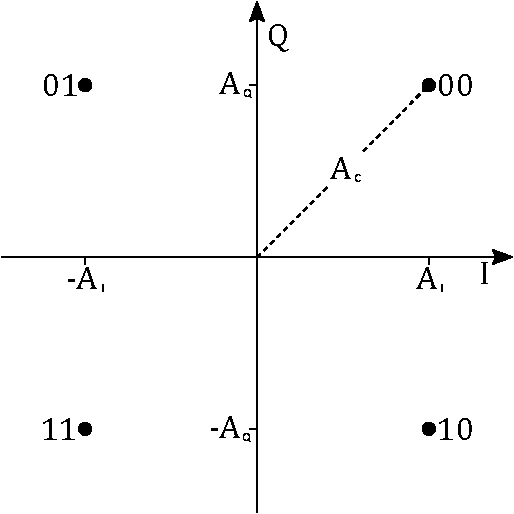
\includegraphics[width=0.5\textwidth]{./sdf/m_qam_system/figures/constellation.pdf}
	\caption{4-QAM constellation points.}
	\label{fig:const}
\end{figure}

%M can take several values: $2, 4, 16, 32, ...$. The first two correspond to BPSK and QPSK modulation, respectively.

\subsection{Theoretical Analysis}

M-QAM is a modulation scheme that takes advantage of two sinusoidal carriers
with a phase difference of $\pi/2$. The resultant output consists of a signal
with both amplitude and phase variations. The two carriers, referred to as I
(In-phase) and Q (Quadrature), can be represented as

\begin{align}
	I(t)=a(t)\cos(\phi t) \\
	Q(t)=a(t)\sin(\phi t)
\end{align}

which means that any sinusoidal wave can be decomposed in its I and Q components:

\begin{align}
	A_c\cos(\omega~t+\phi)&=A\left(\cos(\omega~t)\cos(\phi)-\sin(\omega~t)\sin(\phi)\right) \\
	&=A_I\cos(\omega~t)-A_Q\sin(\omega~t),
\end{align}

where we have used the expression for the cosine of a sum and the definitions of $A_I$ and $A_Q$.

For the particular case of $M=4$, it can be considered that $A=A_I=A_Q$. If it
is assumed there is no crosstalk or interference between the Q and I components,
the signal can be treated as a pair of independent BPSK systems, one for the
in-phase component and another for the quadrature component.
Using Gray coding, adjacent symbols differ by only one bit. As such, an error in a single component leads to a single bit error.
This means that the probability of an error in bit detection is independent
among components, as there is no crosstalk or interference. That being the case,
the bit error rate can be calculated for the BPSK case.

%Considering a signal with amplitude $A$ sampled at the signal peak with no inter-symbol interference, and affected by noise with variance $n_0/2$, the sampled value will be a Gaussian random variable with mean $\pm A$ and variance $n_0/2$. Thus, the probability of error is given by the probability that the value is affected by a deviation greater than $m$.

Let the $s(t)$ be the signal to be sampled at a given instant $t$ for either the
in-phase or quadrature component, $a(t)$ be the component corresponding to the
transmitted signal with peak amplitude equal to $A$, depending on whether the
transmitted signal was 1 or 0, and $n(t)$ the component associated with the
Gaussian white noise with spectral density $G_n(f) = n_0/2$, such that:

\begin{equation}\label{eq:sigAmpNoise}
s(t) = a(t) + n(t)
\end{equation}

\begin{figure}[H]
	\centering
	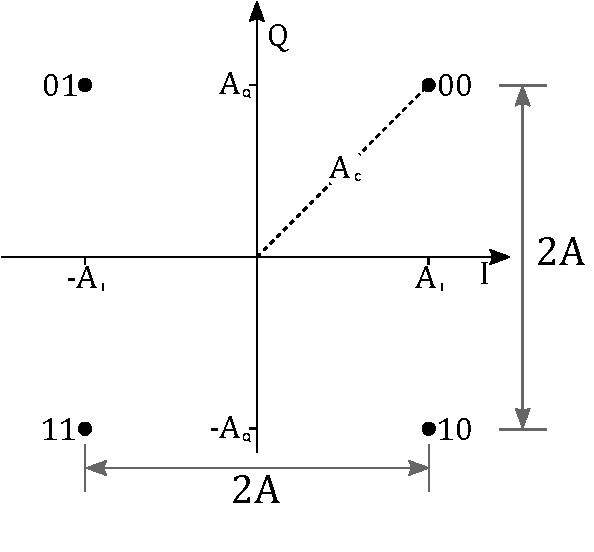
\includegraphics[width=0.5\textwidth]{./sdf/m_qam_system/figures/constellation_d.pdf}
	\caption{The relation between $A$ and the distance between constellation points.\label{fig:const_2m}}
\end{figure}

In this case, assuming the absence of inter-symbol interference, $s(t)$ at the
time of sampling will be a Gaussian random variable with average value of $\pm
A$, depending on what signal was transmitted, and variance equal to $N$, the
noise power. In this case, using the constellation from
Figure~\ref{fig:const_2m}, with a decision boundary halfway between $A$ and
$-A$, an error occurs in two situations: when the a 0 is transmitted but a 1 is
identified, or a 1 is transmitted and a 0 is identified. These errors happen
when the perturbation in the signal due to noise is enough to push the value
beyond the decision boundary. This is illustrated in Figures~\ref{fig:gauss}
and~\ref{fig:gausserr}, where the probability of error is shown by the colored
area under the curve~\cite{schwartz90}.


\begin{figure}[H]
	\centering
	\centering
	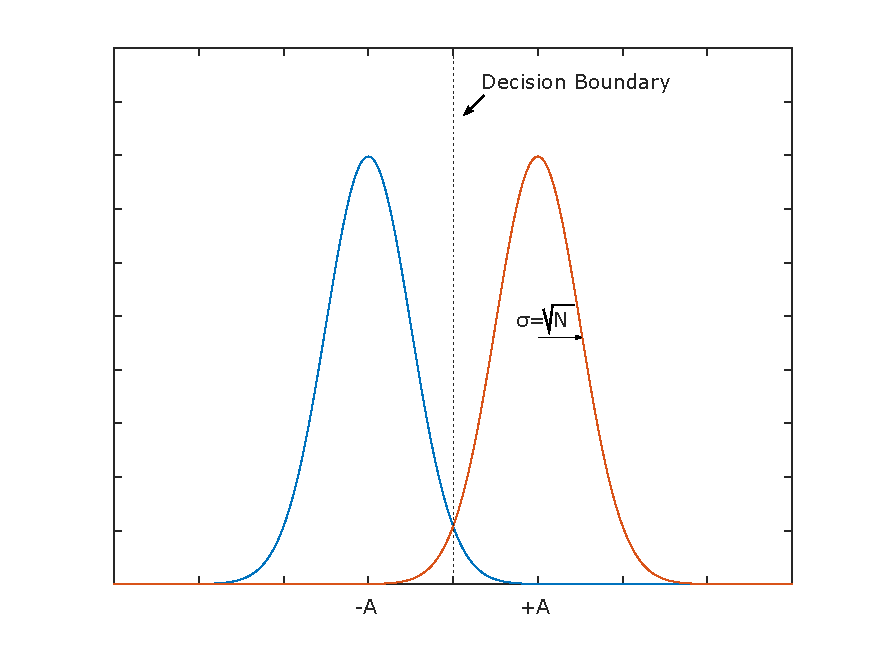
\includegraphics[ width=0.8\textwidth]{./sdf/m_qam_system/figures/gaussians.pdf}
	\caption{Probability density functions for $s(t) = a(t) + n(t)$, with $a(t)=\pm A$ and $n(t)$ as a Gaussian variable of zero mean and variance $N$.}
	\label{fig:gauss}
\end{figure}

\begin{figure}[H]
	\centering
	\begin{subfigure}{.5\textwidth}
		\centering
		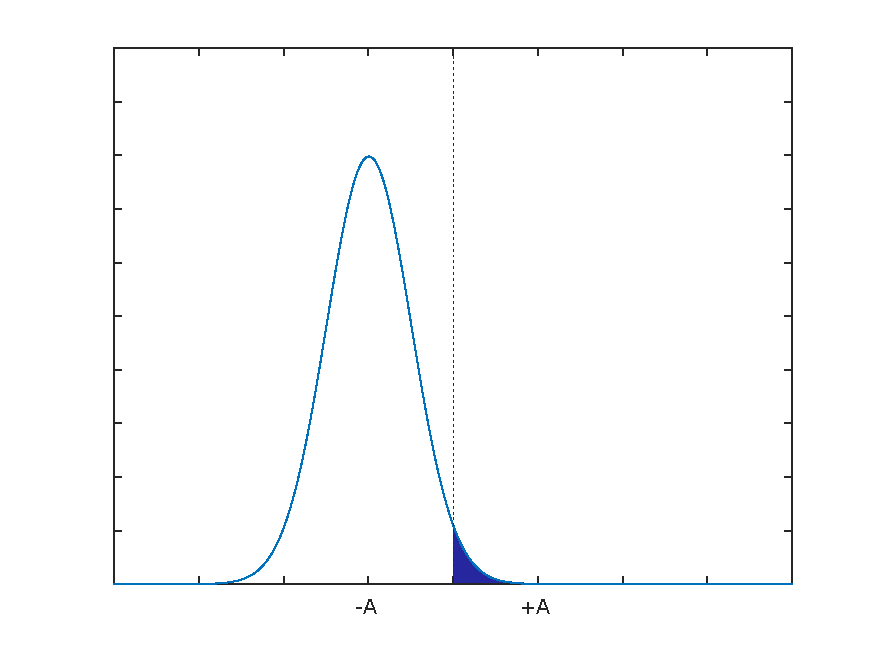
\includegraphics[clip, trim=1cm 0cm 1cm 0cm,width=\textwidth]{./sdf/m_qam_system/figures/gaussian_error_2.pdf}
	\end{subfigure}%
	\begin{subfigure}{.5\textwidth}
		\centering
		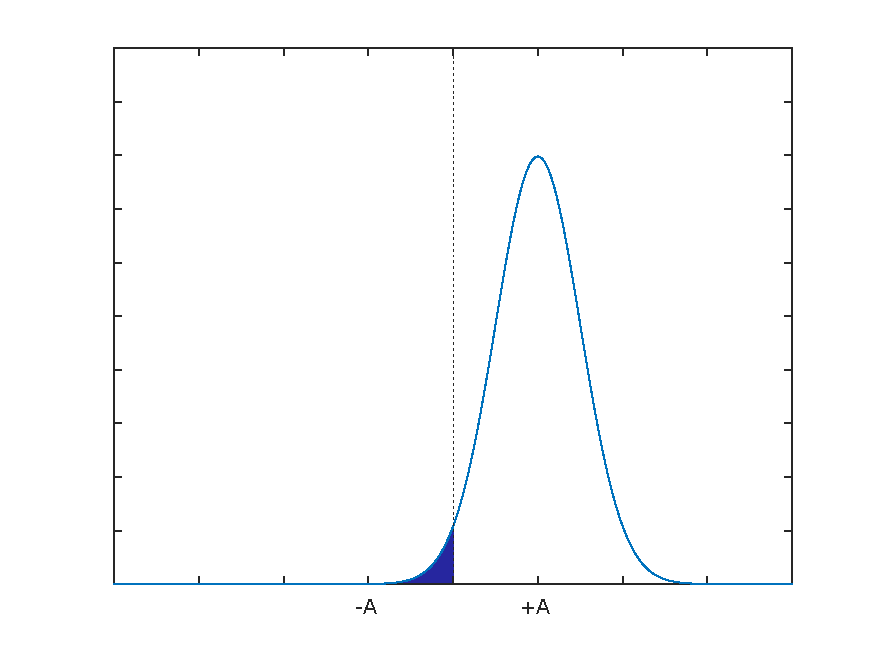
\includegraphics[clip, trim=1cm 0cm 1cm 0cm,width=\textwidth]{./sdf/m_qam_system/figures/gaussian_error.pdf}
	\end{subfigure}
	\caption{The area below the curves represents the probability of error for each transmitted bit.}
	\label{fig:gausserr}
\end{figure}

The probability of bit error can be expressed as:

\begin{equation}
P_{be} = P_0 P_{e0} + P_1 P_{e1}
\end{equation}

With equal probability for both bits, and considering the constellation's symmetry

\begin{equation}\label{eq:berMQAM}
P_{be} =  Q\left({\frac{A}{\sqrt{N}}}\right) = \frac{1}{2} \text{erfc}\left({\frac{A}{\sqrt{2 N}}}\right)
%= \frac{1}{2} \text{erfc}\left({\frac{A}{\sqrt{n_0}}}\right)
\end{equation}


%\begin{equation}
%P_b= Q\left(\sqrt{\frac{E_b}{n_0}}\right) = \frac{1}{2} erfc\left(\sqrt{\frac{E_b}{2 n_0}}\right).
%\end{equation}

%\begin{equation}\label{eq:berBPSK}
%P_{BE}= Q\left({\sqrt{\frac{2 E_b}{N_0}}}\right) = \frac{1}{2} \text{erfc}\left({\sqrt{\frac{ E_b}{N_0}}}\right).
%\end{equation}

%\begin{equation}\label{eq:berBPSK}
%BER= Q\left({G_{ele}\sqrt{\frac{2 P_L P_S}{n_0}}}\right) = \frac{1}{2} \text{erfc}\left({G_{ele}\sqrt{\frac{P_L P_S}{n_0}}}\right).
%\end{equation}

with


\begin{eqnarray}
&A &= K_{ele} \sqrt{P_L P_S}\label{eq:bpskamplitude}\\
%&N &\propto n_0 B
&N & = n_0 B\label{eq:noiseBw}
%&N & = 2 \frac{n_0}{2} B\label{eq:noiseBw}
\end{eqnarray}
%\begin{equation}\label{eq:berBPSK}
%BER= Q\left({G_{ele}\sqrt{\frac{2 P_L P_S}{n_0}}}\right) = \frac{1}{2} \text{erfc}\left({G_{ele}\sqrt{\frac{P_L P_S}{n_0}}}\right).
%\end{equation}

\noindent where $P_L$ is the local oscillator power, $P_S$ is the average
optical power of the laser source on which the signal is modulated, $K_{ele}$ is
the transimpedance amplifier's gain, $n_0/2$ is the noise spectral density and
$B$ is the channel bandwidth. $A$ is the magnitude of the signal at sampling
time and $\sqrt{N}$ is the RMS noise. Figure~\ref{fig:const_2m} shows the
relation between the constellation points and $A$.

The symbol error rate depends on both bits being correctly detected. This probability is:

\begin{equation}
P_C = (1 - P_{be})^2
\end{equation}

From this, the probability of symbol error is:

\begin{eqnarray}
&P_s &= 1-P_C \nonumber\\
&	   &= 1 - \left(1 - Q \left({\frac{A}{\sqrt{2N}}}\right)\right)^2 \nonumber \\
&	   &= 2 Q\left({\frac{A}{\sqrt{2N}}}\right)\left[1-\frac{1}{2} Q \left({\frac{A}{\sqrt{2N}}}\right)\right]
\end{eqnarray}


%$N_0$ will be the standard deviation of the sampled values.
The peak power signal-to-noise ratio, defined as the ratio between the
instantaneous peak signal power to mean noise power, is given
by~\cite{schwartz90}:

\begin{equation}
	\text{SNR} = \frac{A^2}{{N}}
\end{equation}

\noindent	$N$, the mean noise power, is the variance of the noise signal. The
square root of this value is the peak signal-to-rms-noise ratio, and it is the
single parameter on which the probability of errors depends.

\begin{equation}
\text{SNR}_{RMS} = \frac{A}{\sqrt{N}}
\end{equation}

Here, A is the peak signal amplitude and $\sqrt{N}$ is the RMS noise in the
absence of a signal. Here it is assumed that the electric filter's bandwidth is
large enough for the signal not to be affected, thus limiting only the noise
power.

It's worth noting that optical noise is being ignored in this analysis. The
conditions considered here assume only the presence of electrical noise
appearing at the receiver, as shown if figure~\ref{fig:lodiagram}. In these
conditions, the noise is considered to be independent from the local oscillator.
If there was a noise source in the optical domain, this would not be so.

\begin{figure}[H]
	\centering
	\centering
	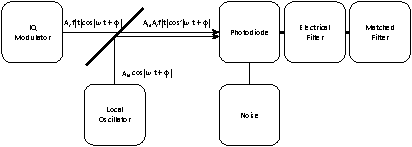
\includegraphics[ width=0.8\textwidth]{./sdf/m_qam_system/figures/LOdiagram.pdf}
	\caption{Local oscillator and receiver filters diagram.}
	\label{fig:lodiagram}
\end{figure}

It is possible to decrease the SNR and, consequently, the error rate reducing
the filter's bandwidth and finding an optimum filter. This filter is called a
matched filter. The resulting signal will still have Gaussian noise, but the
signal-to-noise ratio will be greatly improved. This can be achieved by using a
root-raised cosine filter at the pulse shaper and a similar one at the receiver,
before the sampler. Inter-symbol interference will still be null as it is
equivalent to a raised cosine filter, where half the filtering is done on the
transmitter side (while pulse-shaping) and the other half is done on the
receiver side, before sampling.

%As the constellation remains the same, the expression to calculate the BER is similar, but replacing the values of $m$ and $N_0$ of Equation~\eqref{eq:berMQAM} by those corresponding to the signal at the output of the filter, which can be calculated as:
Considering a pulse with composition similar to the signal described by
Equation~\ref{eq:sigAmpNoise}, let $ a(t) = A_p~p(t) $, where $A_p$ is the peak
amplitude of the signal and $p(t)$ is the shape of the pulse, and $n(t)$ be AWGN
of spectral density $G_n(f) = \frac{n_0}{2}$. Also, let $H(f)$ be the frequency
domain response of the filter at the receiver.
The filter is similar to the shape of the pulse , but reversed in time and shifted by a time delay, such that it maximizes the SNR~\cite{carlson86}.

The energy contained in the pulse that enters the receiver filter depends on the
pulse amplitude and on its shape, and it is given by:

\begin{eqnarray}\label{eq:pulseEnergy}
E_p = \int_{-\infty}^{\infty} {|A(f)|}^2 df = A_p^2 \int_{-\infty}^{\infty} {|P(f)|}^2 df
\end{eqnarray}

The amplitude of the signal component after the receiver filter $H(f)$, at a given sampling time $t=t_0+t_d$, is:

\begin{eqnarray}
A_o = \mathfrak{F}^{-1}\left[H(f) A(f)\right]\big|_{t=t_0+t_d} = A_p \int_{-\infty}^{+\infty} H(f) P(f) e^{+j \omega t_d}df
\end{eqnarray}

Similarly, the noise power at the receiver filter output is given by:

\begin{eqnarray}
N_o = \int_{-\infty}^{+\infty} {|H(f)|}^2 G_n(f) df = \frac{n_0}{2} \int_{-\infty}^{+\infty} {|H(f)|}^2
\end{eqnarray}

This means that the peak signal power to mean noise power ratio at the filter output is given by:

\begin{eqnarray}
\frac{A_o^2}{N_o} &= A_p^2 \frac{\big|\int_{-\infty}^{+\infty} |H(f) P(f)e^{j\omega t_d} df\big|^2}{\int_{-\infty}^{+\infty} {|H(f)|}^2 G_n(f) df}\\\nonumber
				  &= A_p^2 \frac{\big|\int_{-\infty}^{+\infty} |H(f) P(f)e^{j\omega t_d} df\big|^2}{\frac{n_0}{2}\int_{-\infty}^{+\infty} {|H(f)|}^2df}
\end{eqnarray}

It can be shown that a matched filter maximizes the ratio above, so that it becomes~\cite{carlson86} :

\begin{equation}
\frac{A_o^2}{N_o} = \frac{A_p^2}{n_0/2} \int_{-\infty}^{+\infty} |P(f)|^2 df = \frac{A_p^2}{n_0/2} \int_{-\infty}^{+\infty} p(t)^2 dt
\end{equation}

Substituting from equation~\ref{eq:pulseEnergy}:

\begin{equation}
\frac{A_o^2}{N_o} = \frac{2 E_p}{n_0}
\end{equation}

This shows that the SNR and, therefore, the error probability are dependent on
the energy of each symbol and the noise spectral density. However, even though
the relation does not directly depend on the pulse shape, the energy of each
symbol still depends on the pulse shape. The energy of the symbol results from
an integration over the symbol period.
% Considering two a similar shaped pulses, with similar amplitude but duration, the one with longer duration should have more energy.

The BER expression for matched filtering the becomes:

\begin{equation}\label{eq:berMQAMmf}
P_{be} =  Q\left(\sqrt{\frac{2 E_p}{{n_0}}}\right) = \frac{1}{2} \text{erfc}\left(\sqrt{\frac{E_p}{n_0}}\right)
%= \frac{1}{2} \text{erfc}\left({\frac{A}{\sqrt{n_0}}}\right)
\end{equation}

To exemplify with a simple case, let the pulse shape be rectangular with period $T_s$, such as:

\begin{equation*}
	a(t) = \begin{cases}
		A               & 0 \le t \le T_s\\
		0               & t > T_s\\
	\end{cases}
\end{equation*}

The energy of a pulse at the receptor input will be given by:

\begin{equation}
E_p = \int_{0}^{T_s} {a(t)^2cos^2(\omega_0 t)} dt
\end{equation}

If $\omega_0$ is such that $\omega_0 T_s \gg 1$, as it typically is when modulating optical signals, $cos^2(\omega_0 t) \doteq 1/2$. Then:

\begin{equation}\label{eq:rectSigEn}
E_p \doteq \frac{1}{2}\int_{0}^{T_s} a(t)^2 dt = \frac{1}{2}\int_{0}^{T_s} A^2 p(t)^2 dt=\frac{1}{2} A^2 \int_{0}^{T_s} p(t)^2 dt= \frac{A^2 T_s}{2}
\end{equation}

Substituting from equations~\ref{eq:noiseBw} and~\ref{eq:rectSigEn} into Equation~\ref{eq:berMQAMmf}, the BER expression becomes:

\begin{equation}\label{eq:berMod}
P_{be} = \frac{1}{2} \text{erfc}\left(\sqrt{\frac{A^2 T_s / 2}{ N / B}}\right) =
\frac{1}{2} \text{erfc}\left(\frac{A}{\sqrt{2N}} \sqrt{{T_s}{B}}\right) =
\frac{1}{2} \text{erfc}\left(\frac{A}{\sqrt{2N}} \sqrt{\frac{B}{R_s}}\right)
%= \frac{1}{2} \text{erfc}\left({\frac{A}{\sqrt{n_0}}}\right)
\end{equation}

%Similarly, let the signal be shaped using a root-raised-filter, defined as the square root of a raised-cosine in the frequency domain. It ca defined as:

%\begin{equation}
%	RRC(f) = \begin{cases}
%	1              & |f| \le \frac{1-\beta}{2T_s}\\
%	1 cos\left[\frac{\pi T_s}{2 \beta}\left( |f| - \frac{1-\beta}{2T_s}\right)\right]               & \frac{1-\beta}{2T_s} \le |f| \le \frac{1+\beta}{2T_s}\\
%	0						   & |f|  \ge \frac{1+\beta}{2T_s}
%	\end{cases}
%\end{equation}
%
%The energy of a signal

%In the case of QPSK with m=4, both the quadrature and in-phase components have $a(t) = \pm A$. The values that replace $A$ and $N_0$ in Equation~\ref{eq:berMQAM} become:

%\begin{eqnarray}
%%&A_{mf} &= \frac{A T}{2} = \frac{G_{ele} T_s B \sqrt{P_L P_S}}{2}\\
%%&N_{mf} &= N \frac{T_s B}{2}
%%&A_{mf} &= \frac{A T}{2} = \frac{G_{ele} T \sqrt{P_L P_S}}{2}\\
%%&N_{mf} &= N \frac{T}{2}
%\end{eqnarray}

%Here, $P_L$ is the local oscillator power, $P_S$ is the average optical power of the laser source on which the signal is modulated, $G_{ele}$ is the gain in the transimpedance amplifier, $T_s$ is the symbol period, $B$ is the bandwidth of the system, $A_mf$ is the average amplitude at the sampling points of the signal after amplification without noise, $\sigma_o^2$ is the variance of the noise component of the matched filter output, the and $n_0$ is the noise spectral density.
%
%
%The optimal BER that can be obtained by using matched filtering is then given by:

%%\begin{eqnarray}\label{eq:berBPSK}
%&P_{be} &= Q\left({\frac{A_{mf}}{\sqrt{N_{mf}}}}\right)\nonumber\\
%&		&= \frac{1}{2} \text{erfc}\left({\frac{A_{o}}{\sqrt{2 N_{o}}}}\right)\nonumber\\
%%&	    &= \frac{1}{2} \text{erfc}\left({\frac{A}{\sqrt{N}}\sqrt{\frac{T_s B}{2}}}\right)\\
%&	    &= \frac{1}{2} \text{erfc}\left({\frac{A}{\sqrt{N}}\sqrt{\frac{T}{2}}}\right)\\
%%&	    &= \frac{1}{2} \text{erfc}\left(\sqrt{{\frac{E_b}{n_0}}}\right)\nonumber
%\end{eqnarray}

%with
%
%\begin{eqnarray}
%&A &= G_{ele} \sqrt{P_L P_S}
%%&m_{mf} &= \frac{1}{2} T G_{ele} \sqrt{P_L P_S} \\
%%&E_b &= \frac{A^2 T}{2} \\
%\end{eqnarray}


%\noindent where $T_s$ is the symbol period, $B$ is the bandwidth of the system, $A$ is as defined in Equation~\ref{eq:bpskamplitude}, the peak amplitude of the signal without noise prior to filtering.
%%and $B_e$ is the energy of a single received bit.

Here, $R_s$ is the symbol rate, defined as $1/T_s$. Note that $N$ here is the
noise power at the input of the matched filter, as is the bandwidth $B$ and the
peak amplitude $A$. The expressions for the Bit-Error-Rate in the cases with and
without matched filtering:

\begin{table}[H]
	\centering
	\begin{tabulary}{1.0\textwidth}{|c|c|}
		\hline
		\textbf{Without matched filter}								& \textbf{With Matched Filter} \\ \hline
		$ \frac{1}{2} \text{erfc} \left( \frac{A}{\sqrt{2N}} \right) $	& $ \frac{1}{2} \text{erfc}\left(\frac{A}{\sqrt{2N}} \sqrt{\frac{B}{R_s}}\right)  $ \\ \hline
	\end{tabulary}

	\caption{Comparison between the BER equations for the cases with and without matched filtering.\label{tab:ber_qpsk}}
\end{table}

Figure~\ref{fig:QPSK_th_curves} show the curves for both these equations, with the parameters listed in Table~\ref{tab:thCurves}.
%Here, $T$ is the symbol period.

\begin{table}[H]
	\centering
	\begin{tabular}{|l|l|}
		\hline
		\multicolumn{2}{|c|}{ \textbf{Curve Parameters} } \\
		\hline
		\textbf{Parameter}     & \textbf{Default Value}                                     \\\hline
		%		numberOfBitsGenerated  & $40000$	                                                \\\hline
		bandwidth              & 64 GHz															\\\hline
		symbolRate		       & 4 GBd, 16GBd		\\\hline
		%		samplesPerSymbol       & $16$                                                       \\\hline
		%		symbolRate		       &		\\\hline
		%		pLength                & $5$                                                        \\\hline
		%		iqAmplitudesValues     & $\lbrace~\lbrace-1,~0\rbrace~,~\lbrace1,~0\rbrace~\rbrace$ \\\hline
		outputOpticalPower     & Variable                                                   \\ \hline
		localOscillatorPower   & $0$~dBm                                                    \\ \hline
		%		localOscillatorPhase   & $0$                                                        \\ \hline
		%		transferMatrix         & $\lbrace~\lbrace \frac{1}{\sqrt{2}},~\frac{1}{\sqrt{2}},~\frac{1}{\sqrt{2}},~\frac{-1}{\sqrt{2}} \rbrace~\rbrace$ & \\ \hline
		responsivity           & $1$                                                        \\ \hline
		amplification          & $10^3$                                                     \\ \hline
		noisePower			   & $10^{-6}$~V$^2$                             					\\ \hline
		confidence             & $0.95$                                                     \\ \hline
		theoreticalSNR (before matched filter) &	0 dB								    \\ \hline
		%		midReportSize          & $0$                                                        \\ \hline
	\end{tabular}
	\caption{Parameters for the theoretical curves in Figure~\ref{fig:QPSK_th_curves}.\label{tab:thCurves}}
\end{table}

\begin{figure}[H]
	\centering
	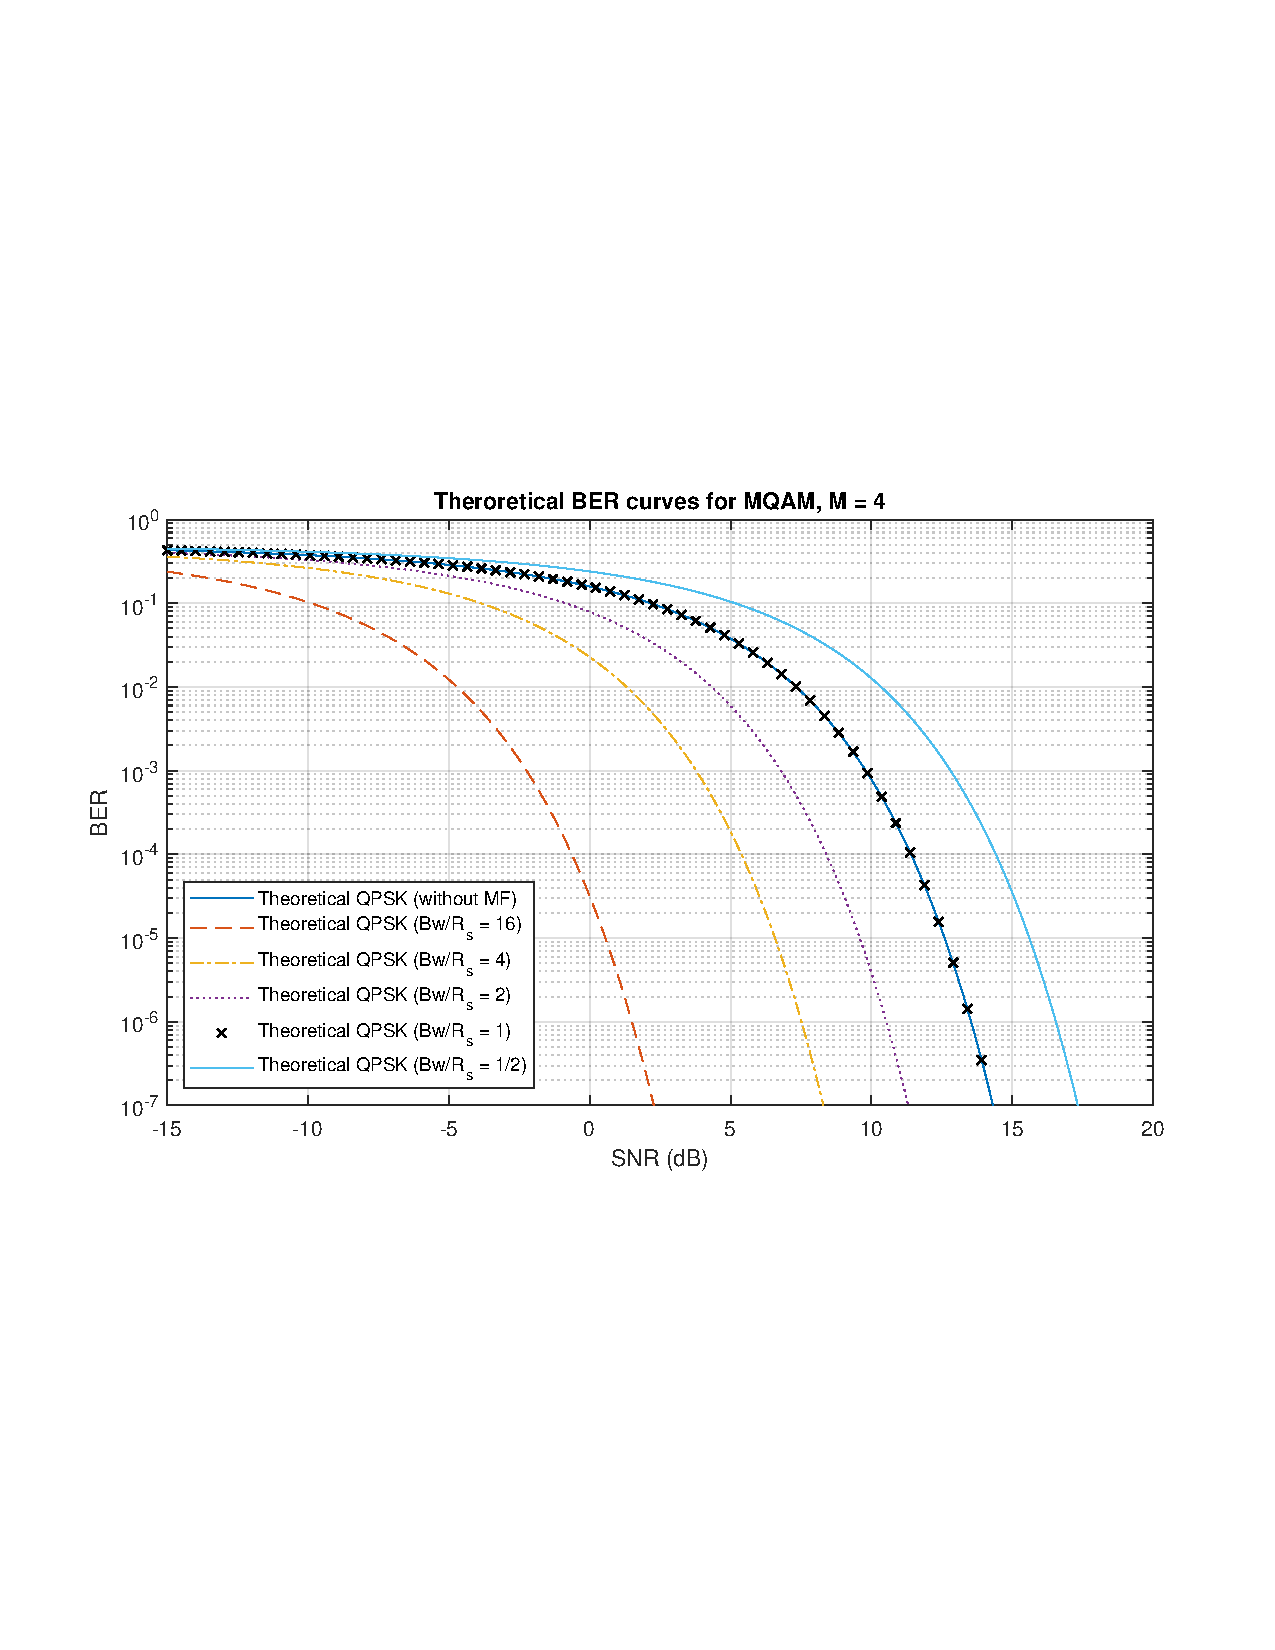
\includegraphics[clip, trim=1cm 8cm 1cm 8cm, width=0.9\textwidth]{./sdf/m_qam_system/figures/teor_BER_curves.pdf}
	\caption{QPSK theoretical BER values as a function of the output optical power in dBm. The bandwidth of the considered system, which limits the overall noise, is defined as a multiple of the sampling rates.\label{fig:QPSK_th_curves}}
\end{figure}


Figure~\ref{fig:QPSK_th_curves} shows the two theoretical curves for QPSK. The
blue one is for QPSK without matched filtering and the red one is using
root-raised-cosine for matched filtering, which provides optimum transmission.
As the use of root-raised-cosine for matched filtering maximizes the
signal-to-noise ratio to its optimal value, it allows achieving the same BER
with much lower optical power. On the blue curve, on the other hand, the
sampling is affected by the full effect of the random noise, as there is no
filtering at the receiver. Because of this, a higher optical power is required
to achieve a similar BER.


It's worth noting that these equations are only valid for M=4, as in that case
the system is similar to QPSK with a 4 point constellation. For $M > 4$ a
different approach is required.

The use of matched filtering should allow transmission with a lower SNR to
achieve the same results as a similar system, even when using a shape with no
inter-symbol interference. This is due to the second filter reducing the noise
impact before detection, while not causing inter-symbol interference or
degradation of the signal data.

\subsection{Simulation Analysis}

\begin{figure}[h]
	\centering
	
\includegraphics[width=1\textwidth]{./sdf/m_qam_system/figures/simulation_mqam}
	\caption{Schematic representation of the MQAM system.}\label{fig:MQAM_system_block_diagram}
\end{figure}


\begin{figure}[h]
	\centering
	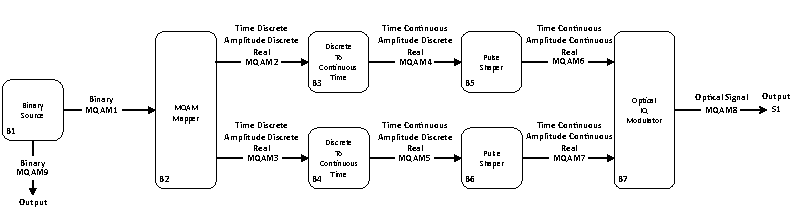
\includegraphics[width=1\textwidth]{./sdf/m_qam_system/figures/simulation_tx}
	\caption{Schematic representation of the MQAM Transmitter block.}\label{fig:simulation_tx}
\end{figure}

%\begin{sidewaysfigure}[h]
%	\centering
%	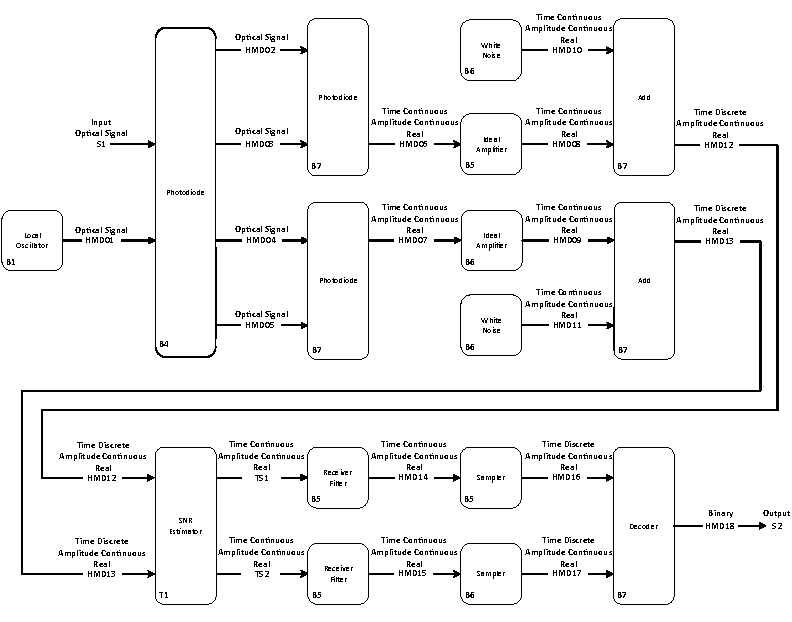
\includegraphics{./sdf/m_qam_system/figures/simulation_rx}
%	\caption{Schematic representation of the Homodyne Receiver block.}\label{fig:simulation_rx}
%\end{sidewaysfigure}

\begin{figure}[H]
	\centering
	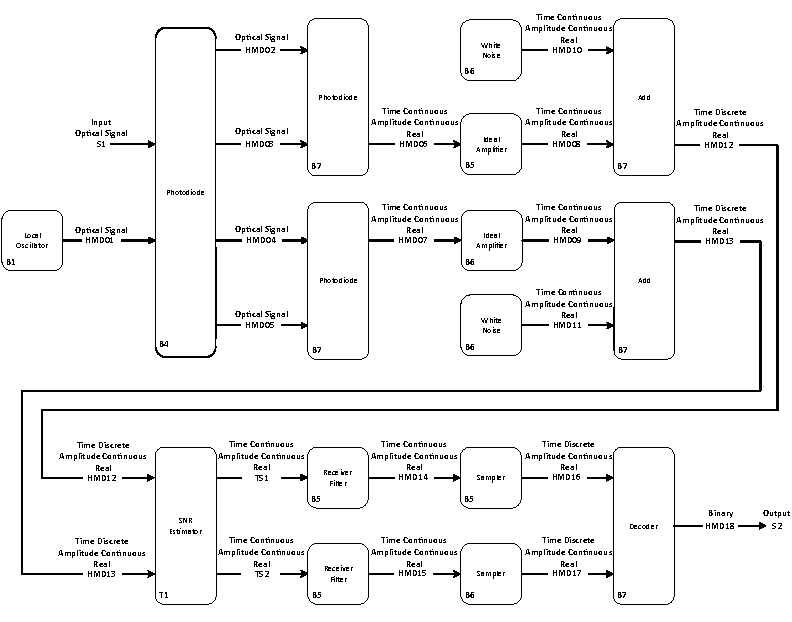
\includegraphics[width=1\textwidth]{./sdf/m_qam_system/figures/simulation_rx}
	\caption{Schematic representation of the Homodyne Receiver block.}\label{fig:simulation_rx}
\end{figure}

The M-QAM transmission system is a complex block of code that simulates the
modulation, transmission and
demodulation of an optical signal using M-QAM modulation.
It is composed of four blocks: a transmitter, a receiver, a sink and a block
that performs a Bit Error Rate (BER) measurement. The schematic representation
of the
system is presented in Figures~\ref{fig:MQAM_system_block_diagram}
to~\ref{fig:simulation_rx}.
	
\paragraph{Current state:} The system currently being implement is a QPSK system (M=4).

\paragraph{Future work:} Extend this block to include other values of M.

\subsection*{Functional description}

A complete description of the M-QAM transmitter and M-QAM homodyne receiver
blocks can be found in the \textit{Library} chapter of this document as well as
a detailed description of the independent blocks that compose these blocks.
The M-QAM transmitter generates one or two optical signals by encoding a binary
string using M-QAM modulation. It also outputs a binary signal that is used to
perform the BER measurement.
The M-QAM homodyne receiver accepts one input optical signal and outputs
a binary signal. It performs the M-QAM demodulation of the input signal by
combining the optical signal with a local oscillator.
The demodulated optical signal is compared to the binary one produced by the
transmitter in order to estimate the Bit Error Rate (BER).
The files used are summarized in tables~\ref{tab:sources} and~\ref{tab:headers}.
These include all blocks and sub-blocks used and allow for the full operation of
the M-QAM system.

\subsection*{Required files}\label{RequiredFilesMQAM}

\begin{table}[H]
    \centering
    \begin{tabulary}{1.0\textwidth}{|p{7.5cm}|p{5.5cm}|p{1cm}|}
        \hline
        \multicolumn{3}{|c|}{ \textbf{Source Files} } \\
        \hline
        \textbf{File}                      			 & \textbf{Comments} & \textbf{Status} \\ \hline
        add\_20171116.cpp                            &                   & \checkmark \\ \hline
        binary\_source\_20180118.cpp                 &                   & \checkmark \\ \hline
        bit\_error\_rate\_20171810.cpp               &                   & \checkmark \\ \hline
        decoder\_20180118.cpp                        &                   & \checkmark \\ \hline
        discrete\_to\_continuous\_time\_20180118.cpp &                   & \checkmark \\ \hline
        homodyne\_receiver\_20171203.cpp             & $^{1}$			 & \checkmark \\ \hline
        ideal\_amplififer\_20180118.cpp              &                   & \checkmark \\ \hline
        iq\_modulator\_20180118.cpp                  &                   & \checkmark \\ \hline
        local\_oscillator\_20180118.cpp              &                   & \checkmark \\ \hline
        m\_qam\_mapper\_20180118.cpp                 &                   & \checkmark \\ \hline
        m\_qam\_system.cpp                 			 & $^{2}$   		 & \checkmark \\ \hline
        m\_qam\_transmitter\_20180118.cpp            &                   & \checkmark \\ \hline
        netxpto\_20180118.cpp                        & $^{2}$ 			 & \checkmark \\ \hline
        optical\_hybrid\_20180118.cpp                &                   & \checkmark \\ \hline
        photodiode\_old\_20180118.cpp                &                   & \checkmark \\ \hline
        pulse\_shaper\_20180118.cpp                  &                   & \checkmark \\ \hline
        sampler\_20171119.cpp                        &                   & \checkmark \\ \hline
        sink\_20180118.cpp                           &                   & \checkmark \\ \hline
        super\_block\_interface\_20180118.cpp        & $^{2}$ 			 & \checkmark \\ \hline
        white\_noise\_20180118.cpp                   & 					 & \checkmark \\ \hline
    \end{tabulary}

    \caption{$^1$ The library entry is under a different name, \textit{m\_qam\_receiver};\\
    $^2$ No library entry as it is a main or general purpose file, not a specific block. 	 \label{tab:sources}}
\end{table}

\begin{table}[H]
    \centering
    \begin{tabulary}{1.0\textwidth}{|p{7cm}|p{6cm}|p{1cm}|}
        \hline
        \multicolumn{3}{|c|}{ \textbf{Header Files} } \\
        \hline
        \textbf{File}                      & \textbf{Comments} & \textbf{Status} \\ \hline
        add\_20171116.h                            & 			   & \checkmark \\ \hline
        binary\_source\_20180118 .h                &                   & \checkmark \\ \hline
        bit\_error\_rate\_20171810.h               &             & \checkmark \\ \hline
        decoder\_20180118.h                        &                   & \checkmark \\ \hline
        discrete\_to\_continuous\_time\_20180118.h &                   & \checkmark \\ \hline
        homodyne\_receiver\_20171203.h             & $^{1}$          & \checkmark \\ \hline
        ideal\_amplifier\_20180118.h               &                   & \checkmark \\ \hline
        iq\_modulator\_20180118.h                  &                   & \checkmark \\ \hline
        local\_oscillator\_20180118.h              &                   & \checkmark \\ \hline
        m\_qam\_mapper\_20180118.h                 &                   & \checkmark \\ \hline
        m\_qam\_transmitter\_20180118.h            &                   & \checkmark \\ \hline
        netxpto\_20180118.h                        & $^2$ 			   & \checkmark \\ \hline
        optical\_hybrid\_20180118.h                &                   & \checkmark \\ \hline
        photodiode\_old\_20180118.h                &                   & \checkmark \\ \hline
        pulse\_shaper\_20180118.h                  &                   & \checkmark \\ \hline
        sampler\_20171119.h                        &               & \checkmark \\ \hline
        sink\_20180118.h                           &                   & \checkmark \\ \hline
        super\_block\_interface\_20180118.h        & $^2$			   & \checkmark \\ \hline
        white\_noise\_20180118.h                   &                   & \checkmark \\ \hline
    \end{tabulary}
    \caption{$^1$ The library entry is under a different name, \textit{m\_qam\_receiver}\\
    $^2$ No library entry as it is a main or general purpose file, not a specific block. \label{tab:headers}}
\end{table}

%\begin{table}[]
%	\centering
%	\caption{Main system files}
%	\begin{tabular}{|c|c|c|c|ccc}
%		\cline{1-4}
%		\textbf{System blocks} & \textbf{Source file} & \textbf{Header file}  &  \textbf{Status} & \\ \cline{1-4}
%		Main & m\_qam\_system\_sdf.cpp & --- & \checkmark & \\ \cline{1-4}
%		M-QAM transmitter & m\_qam\_transmitter\_20180118.cpp & m\_qam\_transmitter\_20180118.h & \checkmark &  \\ \cline{1-4}
%		M-QAM receiver & homodyne\_receiver\_20180118.cpp & homodyne\_receiver\_20180118.h & \checkmark &  \\ \cline{1-4}
%		Sink & sink\_20180118.cpp & sink\_20180118.h &  \checkmark & \\ \cline{1-4}
%		BER estimator & bit\_error\_rate\_20171810.cpp & bit\_error\_rate\_20171810.h & \checkmark &\\ \cline{1-4}
%	\end{tabular}
%	\label{files_table}
%\end{table}

%\subsection*{Required Files}
%
%The required header and source files needed to run this system are summarized in table \ref{table:files}.
%
%\begin{table}
% 	\centering
% 	\caption{Required files}
% 	\begin{tabular}{|c|c|p{40mm}|c|ccp{40mm}c}
% 		\cline{1-4}
% 		\textbf{Header file} & \textbf{Source file} & \textbf{Description} &  \textbf{Status} & \\ \cline{1-4}
% 		add.h & add.cpp & Adds two signals.  & \checkmark &   \\ \cline{1-4}
% 		binary\_source.h & binary\_source.cpp & Produces a binary sequence. & \checkmark & \\ \cline{1-4}
% 		bit\_error\_rate.h & bit\_error\_rate.cpp & Computes the BER and writes it to a text file. & \checkmark & \\ \cline{1-4}
% 		discrete\_to\_continuous\_time.h & discrete\_to\_continuous\_time.cpp & Converts a signal from discrete in time to continuous in time. & \checkmark & \\ \cline{1-4}
% 		homodyne\_receiver.h & m\_qam\_homodyne\_receiver.cpp & & \\ \cline{1-4}
% 		ideal\_amplifier.h & ideal\_amplifier.cpp & Amplifies the signal. & \checkmark & \\ \cline{1-4}
% 		iq\_modulator.h & iq\_modulator.cpp & Divides the signal in its quadrature and in phase components & \checkmark &\\ \cline{1-4}
% 		local\_oscillator.h & local\_oscillator.cpp & & & \checkmark &\\ \cline{1-4}
% 		m\_qam\_mapper.h & m\_qam\_mapper.cpp & Maps the signal using the defined constellation & \checkmark & \\ \cline{1-4}
% 		m\_qam\_transmitter.h & m\_qam\_transmitter.cpp & & \checkmark & \\ \cline{1-4}
% 		netxpto.h & netxpto.cpp & General class that contains definition from signals and buffers. & \checkmark &\\ \cline{1-4}
% 		optical\_hybrid.h & optical\_hybrid.cpp & Implements an optical hybrid. & \checkmark & \\ \cline{1-4}
% 		photodiode\_old.h & photodiode\_old.cpp & Pair of photodiodes and current subtraction. & \checkmark & \\ \cline{1-4}
% 		pulse\_shaper.h & pulse\_shaper.cpp & Electrical filter. & \checkmark &\\ \cline{1-4}
% 		sampler\_20171119.h & sampler\_20171119.cpp & Samples the signal. & \checkmark &\\ \cline{1-4}
% 		sink.h & sink.cpp & Deletes signal. & \checkmark & \\ \cline{1-4}
% 		super\_block\_interface.h & super\_block\_interface.cpp & & \checkmark &\\ \cline{1-4}
% 		white\_noise.h & white\_noise.cpp & Generates white gaussian noise. & \checkmark &\\ \cline{1-4}
% 	\end{tabular}
% 	\label{table:files}
%\end{table}
\pagebreak
\subsection*{Input Parameters}

%The system accepts several input parameters that can be defined by the user. These are described in table \ref{table:in_par}.

\begin{table}[H]
	\centering
	\caption{Input parameters}
	\begin{tabular}{|c|c|p{70mm}|ccp{70mm}}
		\cline{1-3}
		\textbf{Parameter} & \textbf{Type} & \textbf{Description} &    \\ \cline{1-3}
		numberOfBitsGenerated & t\_integer & Determines the number of bits to be generated by the binary source  &    \\ \cline{1-3}
		samplesPerSymbol & t\_integer & Number of samples per symbol &    \\ \cline{1-3}
		prbsPatternLength & int & Determines the length of the pseudorandom sequence pattern (used only when the binary source is operated in \textit{PseudoRandom} mode) &    \\ \cline{1-3}
		bitPeriod & t\_real & Temporal interval occupied by one bit &    \\ \cline{1-3}
		rollOffFactor\_shp & t\_real & Parameter of the pulse shaper filter &    \\ \cline{1-3}
		rollOffFactor\_out & t\_real & Parameter of the output filter &    \\ \cline{1-3}
		shaperFilter & enum & Type of filter used in Pulse Shaper &    \\ \cline{1-3}
		outputFilter & enum & Type of filter used in output filter &    \\ \cline{1-3}
		seedType & enum & Method of seeding noise generators &    \\ \cline{1-3}
		seedArray & array<int,2> & Seeds to initialize noise generators &    \\ \cline{1-3}
		signalOutputPower\_dBm & t\_real & Determines the power of the output optical signal in dBm &  \\ \cline{1-3}
		numberOfBitsReceived & int &   Determines when the simulation should stop. If $-1$ then it only stops when there is no more bits to be sent&   \\ \cline{1-3}
		iqAmplitudeValues & vector<t\_iqValues> & Determines the constellation used to encode the signal in IQ space &    \\ \cline{1-3}
		symbolPeriod & double & Given by bitPeriod/samplesPerSymbol &    \\ \cline{1-3}
		localOscillatorPower\_dBm & t\_real & Power of the local oscillator &    \\ \cline{1-3}
		responsivity & t\_real & Responsivity of the photodiodes (1 corresponds to having all optical power transformed into electrical current) &    \\ \cline{1-3}
		amplification & t\_real & Amplification provided by the ideal amplifier &    \\ \cline{1-3}
		noisePower & t\_real & Average power (and variance) of the white noise &    \\ \cline{1-3}
		samplesToSkip & t\_integer & Number of samples to be skipped by the \textit{sampler} block &    \\ \cline{1-3}
		confidence & t\_real & Determines the confidence limits for the BER estimation &    \\ \cline{1-3}
		midReportSize & t\_integer &  &    \\ \cline{1-3}
		bufferLength & t\_integer & Corresponds to the number of samples that can be processed in each run of the system &    \\ \cline{1-3}
		\end{tabular}
		\label{table:in_par}
		\end{table}

\subsection*{Simulation results}

In this section we show results obtained through the simulations. The
following sections show the eye diagrams of the signal obtained at three
different points in the system: the optical signal S1, the signals after
amplifying the electrical signal and adding the Gaussian white noise HMD12 and
HMD13, and the signal after the filter in the receiver. These eye diagrams will
be shown for a variety of system configurations, with varying noise and
filters, displaying the advantages of using matched filtering with an optimal
filter.

\subsubsection{Without Noise}

These section presents the mentioned eye diagrams in configurations without any
noise added to the signal. This allows studying the effects of inter-symbol
interference caused only by the filters used at the pulse-shaper and at the
receiver,

Figure~\ref{fig:eyespower} shows the eye diagrams for the phase and quadrature 
signals at the IQ modulator and at the receiver. These were obtained using
a raised-cosine filter as a pulse shaper, with a roll-off factor of 0.9. It can
be seen that no inter-symbol interference is present in this case.

\begin{table}[H]
			\centering
			
	\begin{tabular}{|l|l|}
		\hline
		\multicolumn{2}{|c|}{ \textbf{Curve Parameters} } \\
		\hline
		\textbf{Parameter}     & \textbf{Default 
		Value}                                     \\\hline
		%		numberOfBitsGenerated  & 
		%$40000$	                                                \\\hline
		bitPeriod              & 
		$1/32\times10^9$~s														
		\\\hline
%		symbolRate		       
%&                                                     		\\\hline
		samplesPerSymbol       & 
		$16$                                                       \\\hline
		%		symbolRate		       
		%&                                                     		\\\hline
		%		pLength                & 
		%$5$                                                        \\\hline
		%		iqAmplitudesValues     & 
		%$\lbrace~\lbrace-1,~0\rbrace~,~\lbrace1,~0\rbrace~\rbrace$ \\\hline
		outputOpticalPower     & $-120$~dBm (left), $-60$~dBm 
		(right)                       \\ \hline
		shaperFilter	       & 
		RaisedCosine												\\ \hline
		rollOffFactor		   & 
		0.9														\\ \hline
%		localOscillatorPower   & 
%$0$~dBm                                                    \\ \hline
		%		localOscillatorPhase   & 
		%$0$                                                        \\ \hline
		%		transferMatrix         & $\lbrace~\lbrace 
		%\frac{1}{\sqrt{2}},~\frac{1}{\sqrt{2}},~\frac{1}{\sqrt{2}},~\frac{-1}{\sqrt{2}}
		% \rbrace~\rbrace$ & \\ \hline
%		responsivity           & 
%$1$                                                        \\ \hline
%		amplification          & 
%$10^3$                                                     \\ \hline
%		noisePower   & $0$~V$^2$                             					
%\\ \hline
%		confidence             & 
%$0.95$                                                     \\ \hline
		%		midReportSize          & 
		%$0$                                                        \\ \hline
		
	\end{tabular}
\end{table}

\begin{figure}[H]
	\centering
	\textbf{Raised-Cosine Signal (roll-off=0.9) At the Transmitter Output}
	\begin{subfigure}{.5\textwidth}
		\centering
		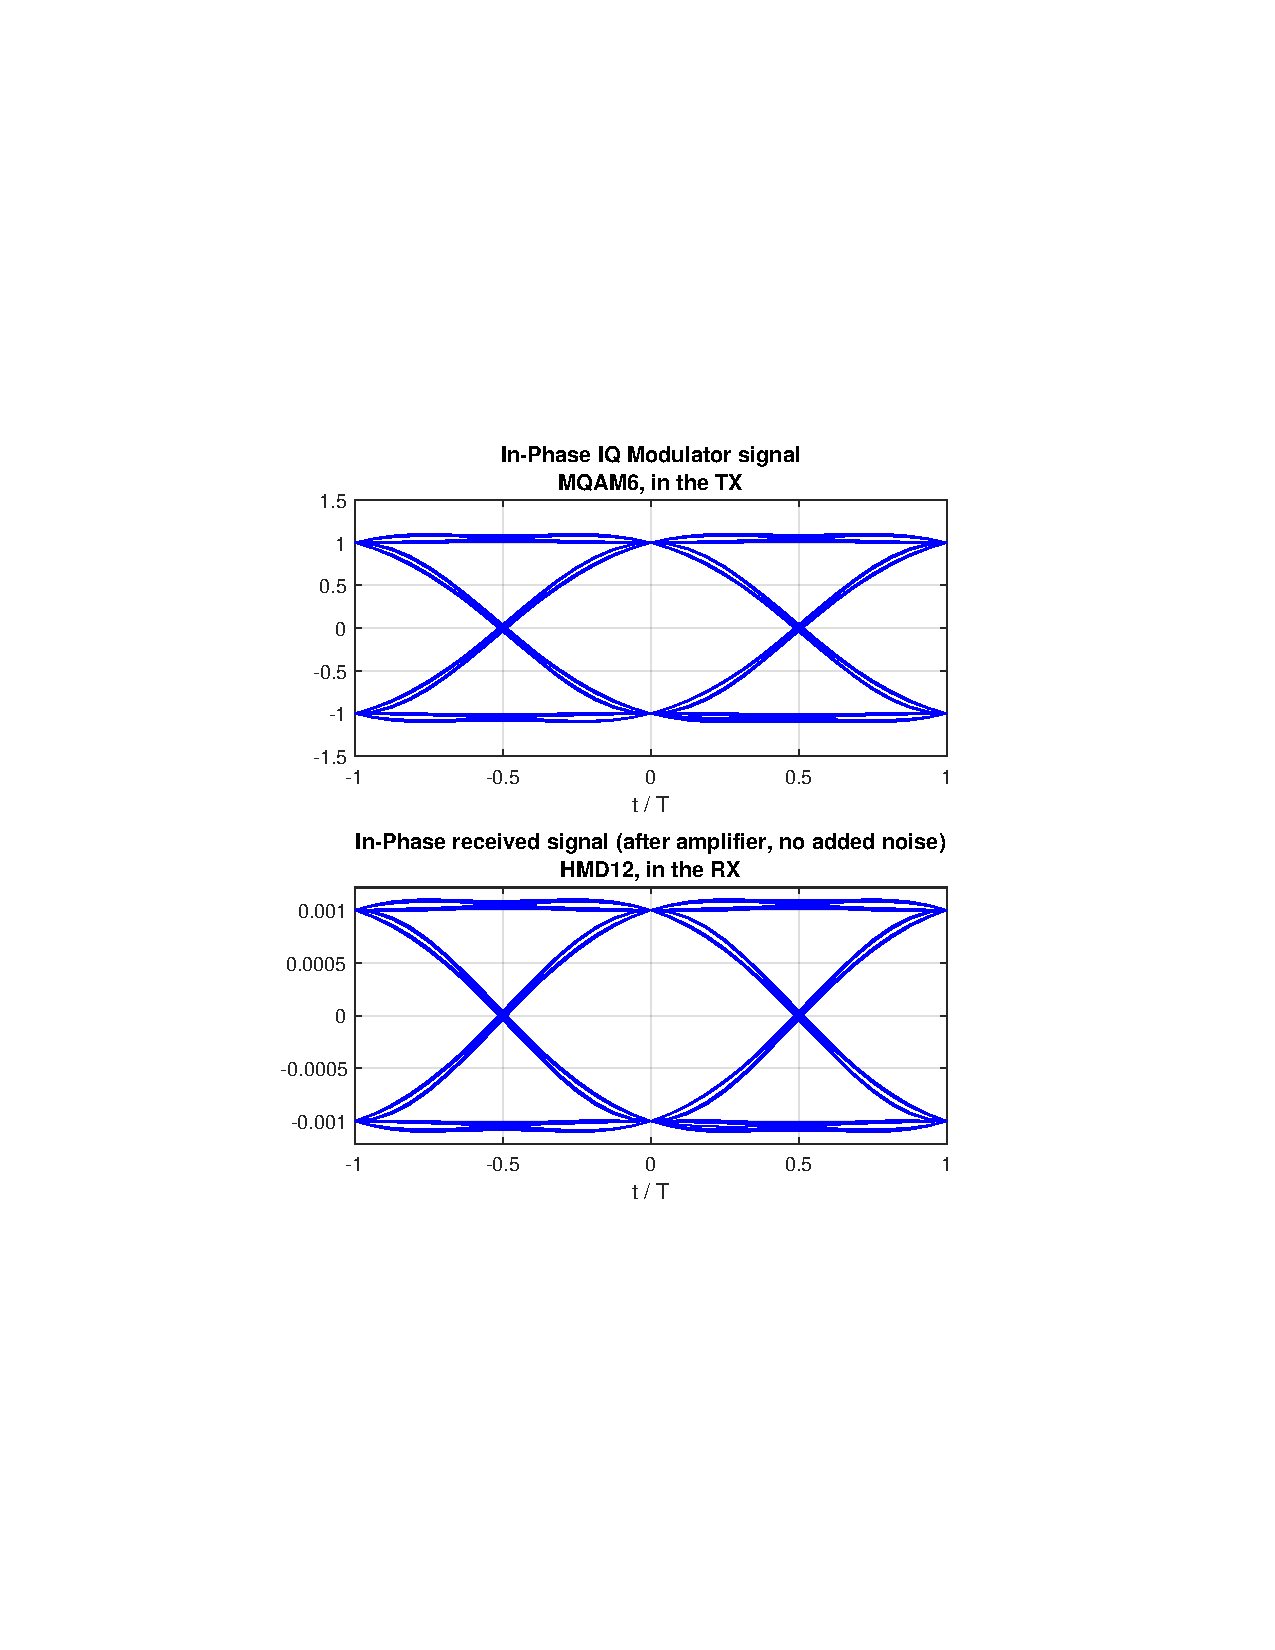
\includegraphics[clip, trim=4cm 7cm 4cm 7cm, width=\textwidth]{./sdf/m_qam_system/figures/eyes/simulRc09Sp60Np00NoMF_i.pdf}
	\end{subfigure}%
	\begin{subfigure}{.5\textwidth}
		\centering
		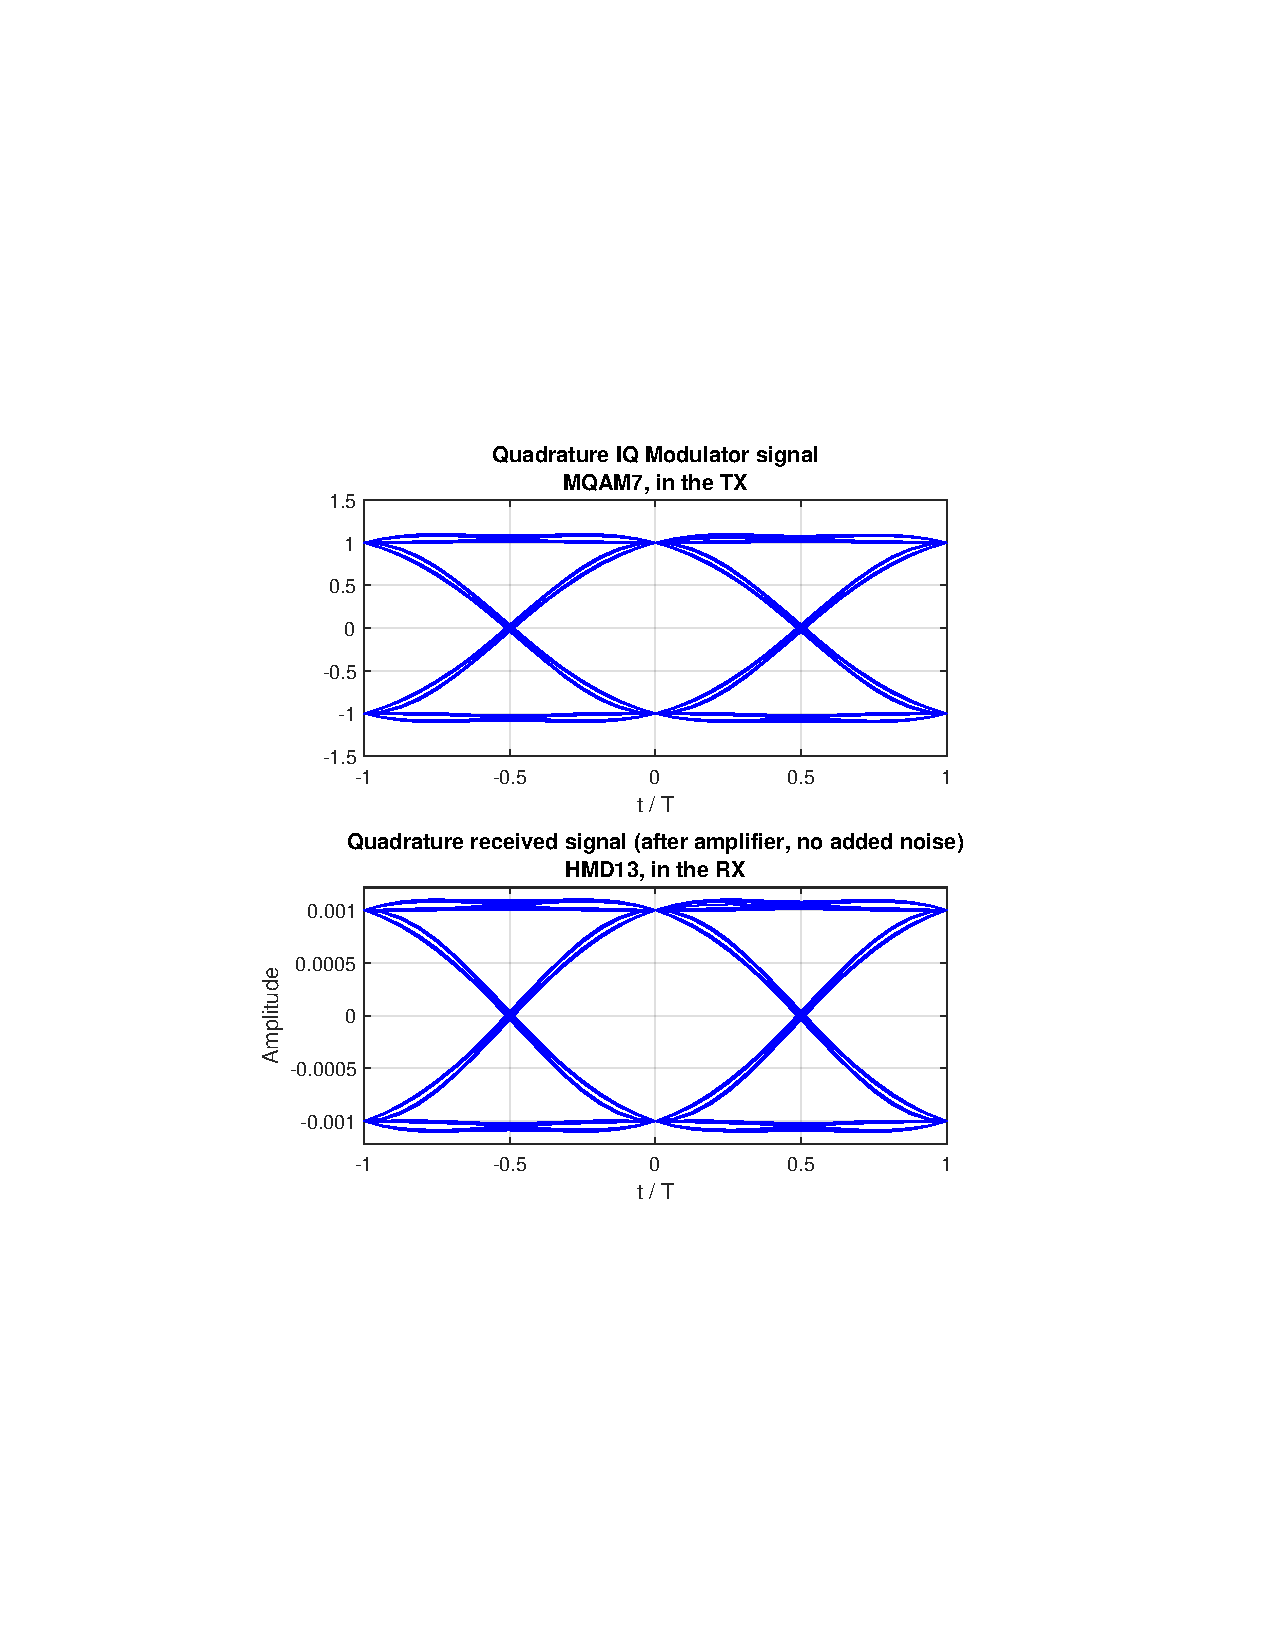
\includegraphics[clip, trim=4cm 7cm 4cm 7cm, width=\textwidth]{./sdf/m_qam_system/figures/eyes/simulRc09Sp60Np00NoMF_q.pdf}
	\end{subfigure}
%	\caption{Eye diagrams for the optical signal at the transmitter output, 
%with an output optical power
%		of $-120~dBm$ (left) and $-60~dBm$ (right) with no added noise. In this 
%case, a raised cosine filter with a roll-off factor of 0.9 was used at the 
%transmitter to shape the signal.}
	\caption{\label{fig:eyespower}}
\end{figure}

As mentioned previously, using matched filters is highly beneficial, as it
allows achieving much lower error rates with the same optical power.

Figure~\ref{fig:eyes_nn_rc_09} shows the eye diagrams of the signal at the
three mentioned points, for a system without any added white noise, while using
matched filtering. The filter used in this case is a raised cosine filter with
a roll-off factor of 0.9. Although this is the ideal filter to use for pulse
shaping, as it does not cause inter-symbol-interference, it can be seen that
when used twice its results are less than ideal, as shown in the eye diagram
captured after the second filter.
\begin{table}[H]
	\centering
	
	\begin{tabular}{|l|l|}
		\hline
		\multicolumn{2}{|c|}{ \textbf{Simulation Parameters} } \\
		\hline
		\textbf{Parameter}     & \textbf{Default Value}                                     \\\hline
		%		numberOfBitsGenerated  & $40000$	                                                \\\hline
		bitPeriod              & $1/32\times10^9$~s														\\\hline
		%		symbolRate		       &                                                     		\\\hline
		samplesPerSymbol       & $16$                                                       \\\hline
		%		symbolRate		       &                                                     		\\\hline
		%		pLength                & $5$                                                        \\\hline
		%		iqAmplitudesValues     & $\lbrace~\lbrace-1,~0\rbrace~,~\lbrace1,~0\rbrace~\rbrace$ \\\hline
		outputOpticalPower     & $-60$~dBm 													\\ \hline
		shaperFilter	       & RaisedCosine												\\ \hline
		outputFilter		   & RaisedCosine												\\ \hline
		rollOffFactor		   & 0.9														\\ \hline
				localOscillatorPower   & $0$~dBm                                                    \\ \hline
				localOscillatorPhase   & $0$                                                        \\ \hline
		%		transferMatrix         & $\lbrace~\lbrace \frac{1}{\sqrt{2}},~\frac{1}{\sqrt{2}},~\frac{1}{\sqrt{2}},~\frac{-1}{\sqrt{2}} \rbrace~\rbrace$ & \\ \hline
				responsivity           & $1$                                                        \\ \hline
				amplification          & $10^3$                                                     \\ \hline
				noisePower   & $0$~V$^2$                             					\\ \hline
		%		confidence             & $0.95$                                                     \\ \hline
		%		midReportSize          & $0$                                                        \\ \hline
	\end{tabular}
\end{table}
\begin{figure}[H]
	\centering
	\textbf{Raised-Cosine Signal (roll-off=0.9) with Matched Filtering}
	\begin{minipage}{\linewidth}
		\centering
	\begin{subfigure}{.45\textwidth}
		\centering
		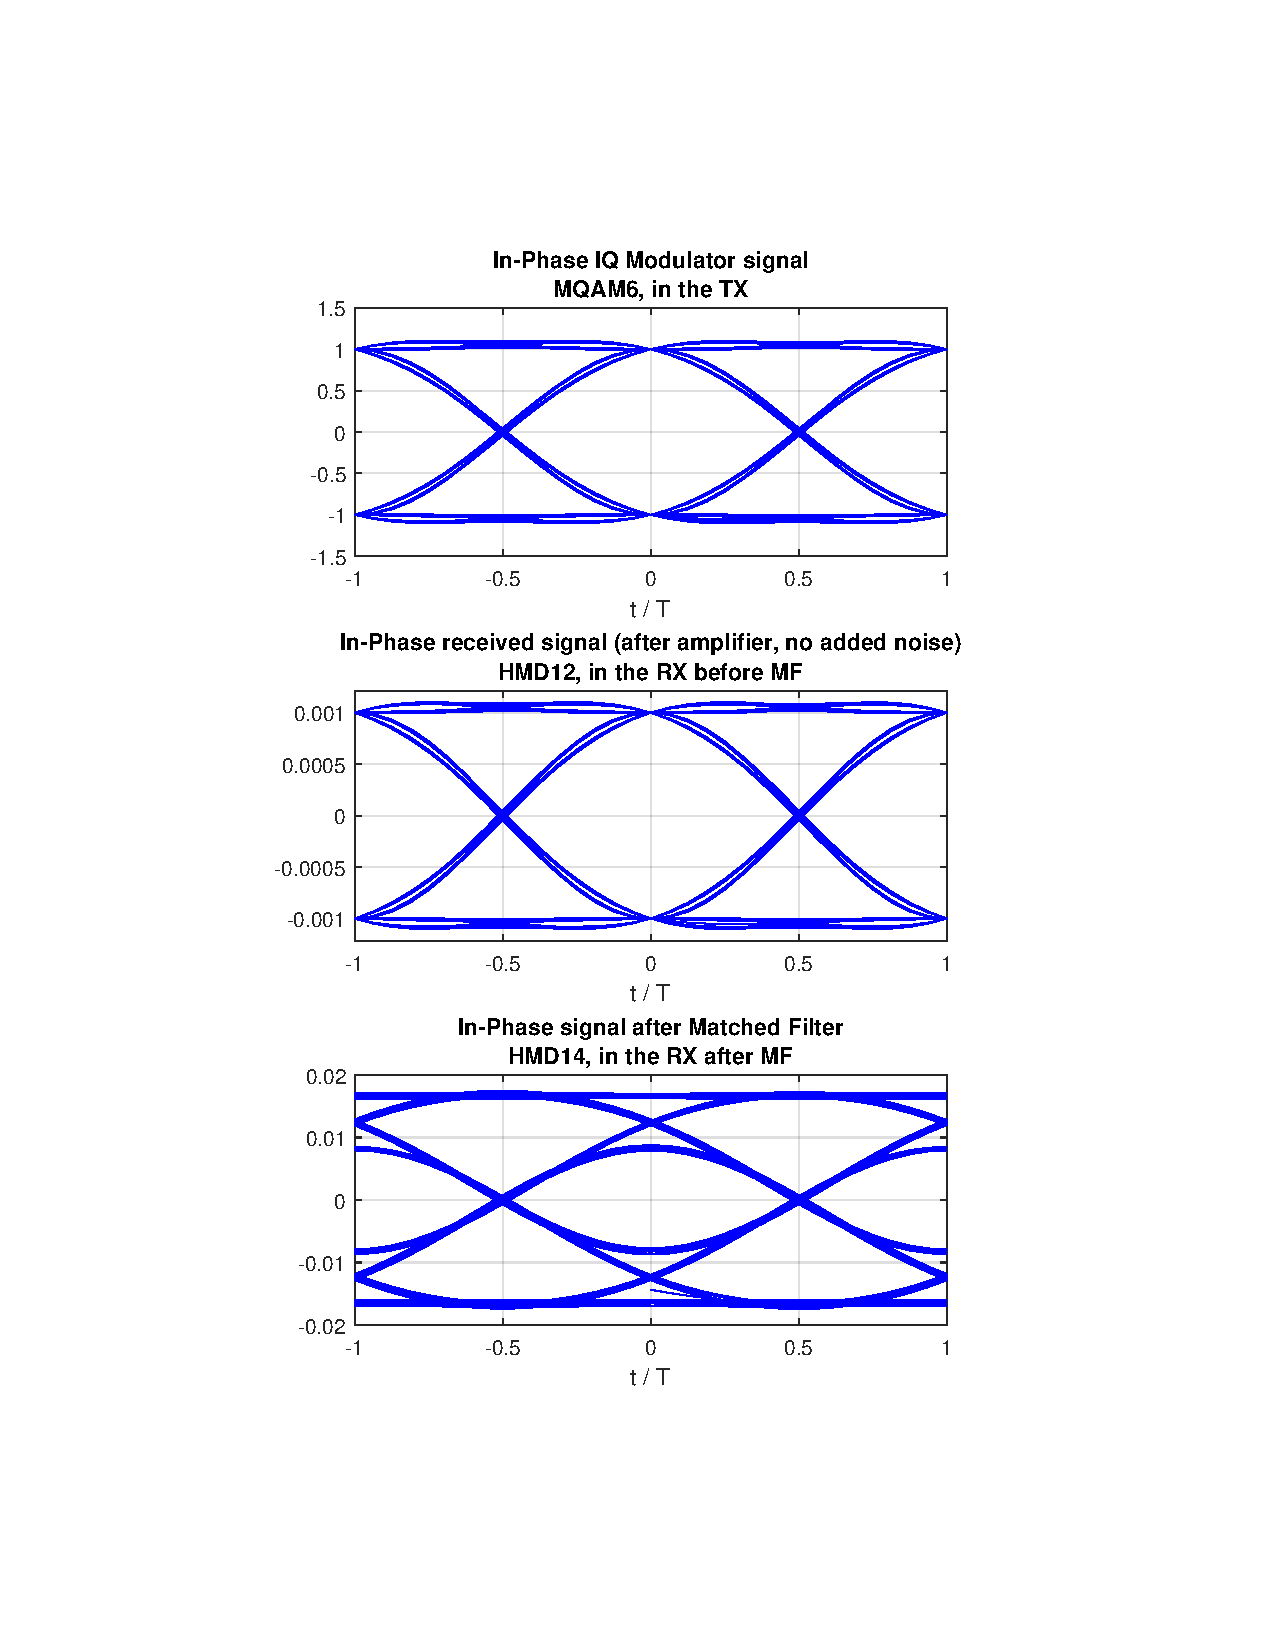
\includegraphics[clip, trim=4cm 4cm 4cm 4cm,
			width=\textwidth]{./sdf/m_qam_system/figures/eyes/simulRc09Sp60Np00_i.pdf}
	\end{subfigure}
	\begin{subfigure}{.45\textwidth}
		\centering
		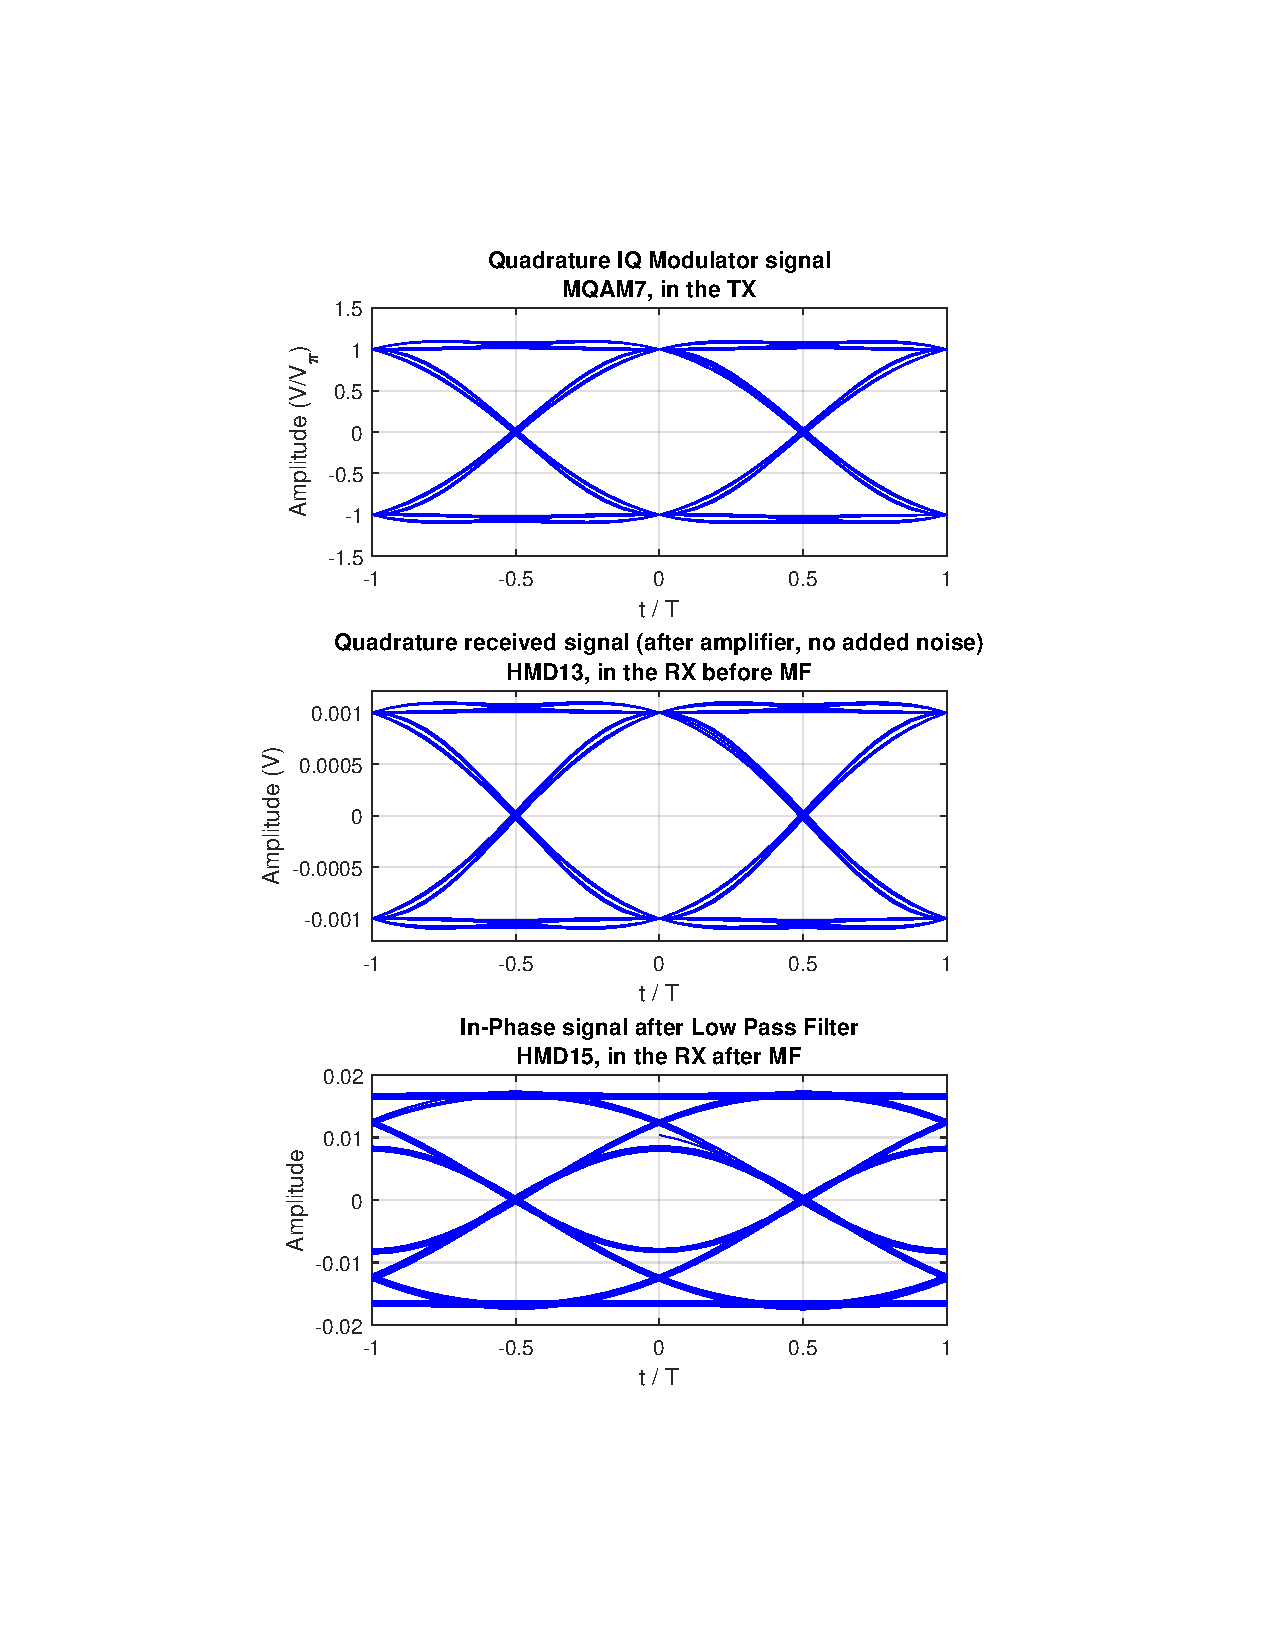
\includegraphics[clip, trim=4cm 4cm 4cm 4cm,
			width=\textwidth]{./sdf/m_qam_system/figures/eyes/simulRc09Sp60Np00_q.pdf}
	\end{subfigure}
	
	\caption{
%		Eye diagrams of the signal using matched filtering with raised-cosine without AWGN.
		Obtained at
		three different points in the system: optical output of transmitter on the top;
		the amplified signal at the middle; and
		after the receiver filter.
%		Simulation done with an optical power output of
%		-60~dBm, 0~dBm at the local oscillator, a gain of $10^3$ at the amplifier, and
%		a rolloff factor of 0.9.
		\label{fig:eyes_nn_rc_09}}
	\end{minipage}
\end{figure}

The optimum solution to achieving no inter-symbol interference while using
matched filtering is to use a root-raised-cosine to do the pulse-shaping at the
transmitter and the filtering at the receiver. The corresponding output of
applying twice a root-raised-cosine is exactly the same as using a
raised-cosine once. As such, the end result suffers from no inter-symbol
interference while reaping the benefits of optimum matched filtering.
Figure~\ref{fig:eyes_nn_rrc_09} shows the eye diagrams when using
root-raised-cosine filter both in the transmitter's pulse-shaper and at the
receiver's filter. The roll-off factor used in both was 0.9. It can be seen
that the shape of the eye diagram is equal to that of
Figure~\ref{fig:eyespower}, which uses a single raised cosine filter at the
pulse-shaper. Thus, it shows no sign of inter-symbol interference.
\begin{table}[H]
	\centering
	
	\begin{tabular}{|l|l|}
		\hline
		\multicolumn{2}{|c|}{ \textbf{Simulation Parameters} } \\
		\hline
		\textbf{Parameter}     & \textbf{Default Value}                                     \\\hline
		%		numberOfBitsGenerated  & $40000$	                                                \\\hline
		bitPeriod              & $1/32\times10^9$~s														\\\hline
		%		symbolRate		       &                                                     		\\\hline
		samplesPerSymbol       & $16$                                                       \\\hline
		%		symbolRate		       &                                                     		\\\hline
		%		pLength                & $5$                                                        \\\hline
		%		iqAmplitudesValues     & $\lbrace~\lbrace-1,~0\rbrace~,~\lbrace1,~0\rbrace~\rbrace$ \\\hline
		outputOpticalPower     & $-60$~dBm 													\\ \hline
		shaperFilter	       & RootRaisedCosine												\\ \hline
		outputFilter		   & RootRaisedCosine												\\ \hline
		rollOffFactor		   & 0.9														\\ \hline
		localOscillatorPower   & $0$~dBm                                                    \\ \hline
		localOscillatorPhase   & $0$                                                        \\ \hline
		%		transferMatrix         & $\lbrace~\lbrace \frac{1}{\sqrt{2}},~\frac{1}{\sqrt{2}},~\frac{1}{\sqrt{2}},~\frac{-1}{\sqrt{2}} \rbrace~\rbrace$ & \\ \hline
		responsivity           & $1$                                                        \\ \hline
		amplification          & $10^3$                                                     \\ \hline
		noisePower   & $0$~V$^2$                             					\\ \hline
		%		confidence             & $0.95$                                                     \\ \hline
		%		midReportSize          & $0$                                                        \\ \hline
	\end{tabular}
\end{table}
\begin{figure}[H]
	\centering

	\textbf{Root-Raised-Cosine Signal (roll-off=0.9) with Matched Filtering}
	\begin{minipage}{\linewidth}
		\centering
	\begin{subfigure}{.45\textwidth}
		\centering
		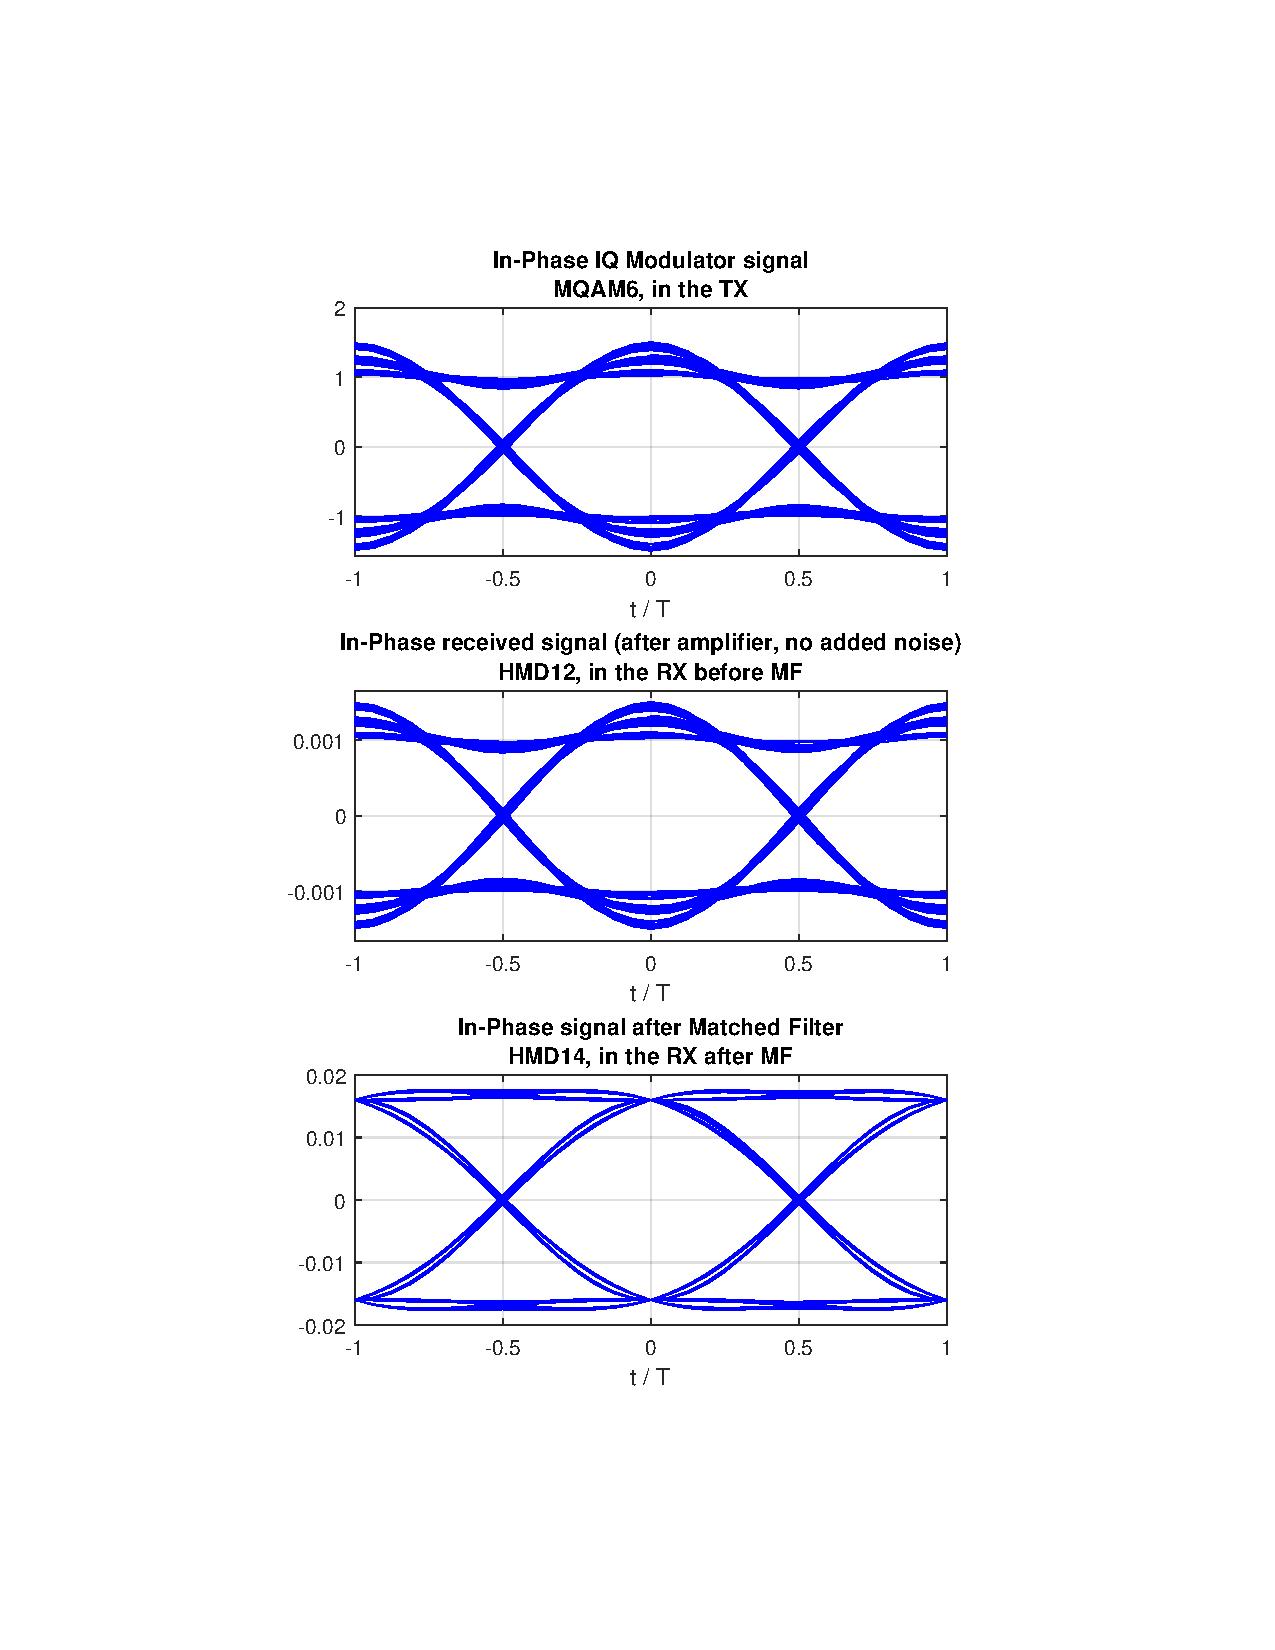
\includegraphics[clip, trim=4cm 4cm 4cm 4cm,
			width=\textwidth]{./sdf/m_qam_system/figures/eyes/simulRrc09Sp60Np00_i.pdf}
	\end{subfigure}
	\begin{subfigure}{.45\textwidth}
		\centering
		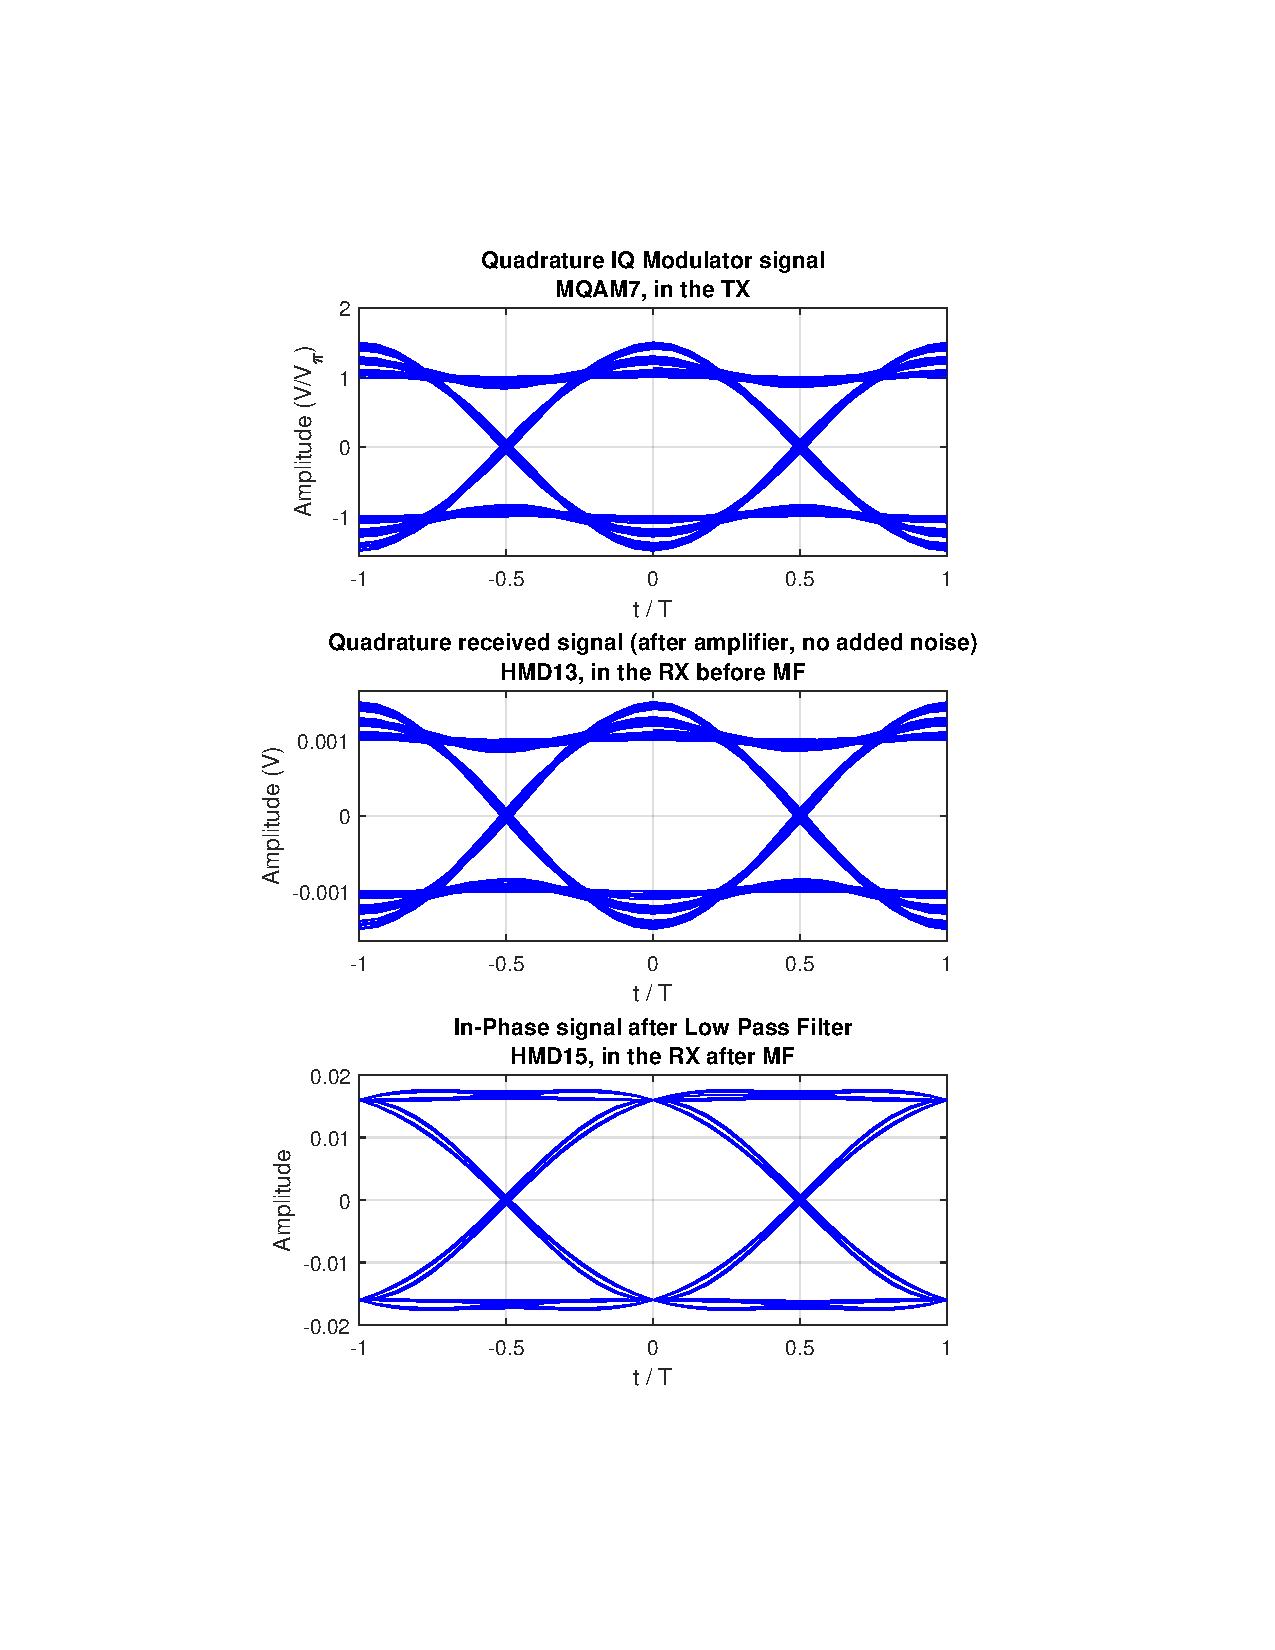
\includegraphics[clip, trim=4cm 4cm 4cm 4cm,
			width=\textwidth]{./sdf/m_qam_system/figures/eyes/simulRrc09Sp60Np00_q.pdf}
	\end{subfigure}
	\caption{
%		Eye diagrams using matched filtering with root-raised-cosine without AWGN.
		Obtained at
		three different points in the system: optical output of transmitter on the top;
		the amplified signal at the middle; and
		after the receiver filter.
%		Simulation done with an optical power output
%		of -60~dBm, 0~dBm at the local oscillator, a gain of $10^3$ at the amplifier,
%		and a rolloff factor of 0.9.
		\label{fig:eyes_nn_rrc_09}}
	\end{minipage}
	
\end{figure}

Figures~\ref{fig:eyes_nn_rrc_03} and~\ref{fig:eyes_nn_rrc_03} show a similar
comparison between matched filtering using raised-cosine or root-raised-cosine
filters, but with a roll-off factor of 0.3. Again, it can be seen that the
final shape of the eye diagram when using the root-raised-cosine for matched
filtering is the same as the shape of the optical signal S1 when using a
raised-cosine-filter.
\begin{table}[H]
	\centering
	
	\begin{tabular}{|l|l|}
		\hline
		\multicolumn{2}{|c|}{ \textbf{Simulation Parameters} } \\
		\hline
		\textbf{Parameter}     & \textbf{Default Value}                                     \\\hline
		%		numberOfBitsGenerated  & $40000$	                                                \\\hline
		bitPeriod              & $1/32\times10^9$~s														\\\hline
		%		symbolRate		       &                                                     		\\\hline
		samplesPerSymbol       & $16$                                                       \\\hline
		%		symbolRate		       &                                                     		\\\hline
		%		pLength                & $5$                                                        \\\hline
		%		iqAmplitudesValues     & $\lbrace~\lbrace-1,~0\rbrace~,~\lbrace1,~0\rbrace~\rbrace$ \\\hline
		outputOpticalPower     & $-60$~dBm 													\\ \hline
		shaperFilter	       & RaisedCosine												\\ \hline
		outputFilter		   & RaisedCosine												\\ \hline
		rollOffFactor		   & 0.3														\\ \hline
		localOscillatorPower   & $0$~dBm                                                    \\ \hline
		localOscillatorPhase   & $0$                                                        \\ \hline
		%		transferMatrix         & $\lbrace~\lbrace \frac{1}{\sqrt{2}},~\frac{1}{\sqrt{2}},~\frac{1}{\sqrt{2}},~\frac{-1}{\sqrt{2}} \rbrace~\rbrace$ & \\ \hline
		responsivity           & $1$                                                        \\ \hline
		amplification          & $10^3$                                                     \\ \hline
		noisePower   & $0$~V$^2$                             					\\ \hline
		%		confidence             & $0.95$                                                     \\ \hline
		%		midReportSize          & $0$                                                        \\ \hline
	\end{tabular}
\end{table}
\begin{figure}[H]
	
		\centering
	\textbf{Raised-Cosine Signal (roll-off=0.3) with Matched Filtering}
	\begin{minipage}{\linewidth}
		\centering
	\begin{subfigure}{.45\textwidth}
		\centering
		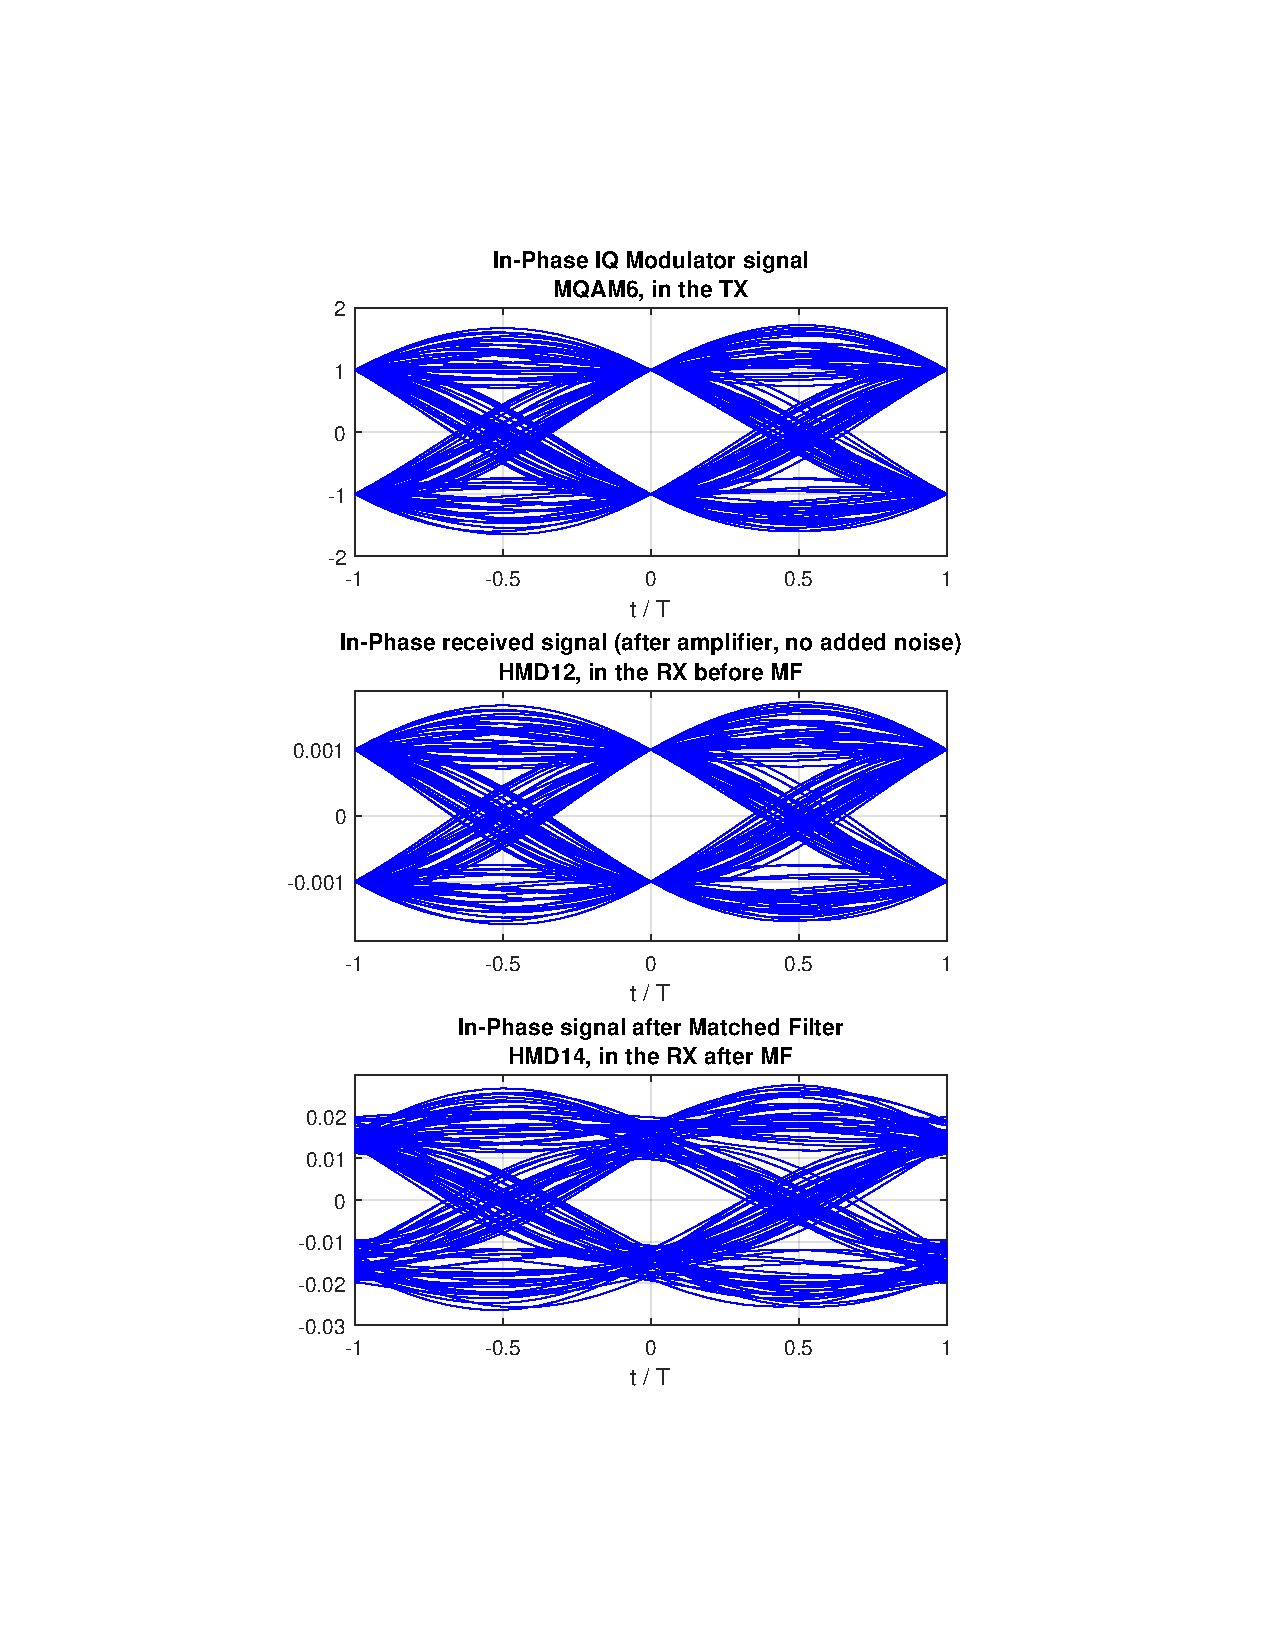
\includegraphics[clip, trim=4cm 4cm 4cm 4cm,
			width=\textwidth]{./sdf/m_qam_system/figures/eyes/simulRc03Sp60Np00_i.pdf}
	\end{subfigure}
	\begin{subfigure}{.45\textwidth}
		\centering
		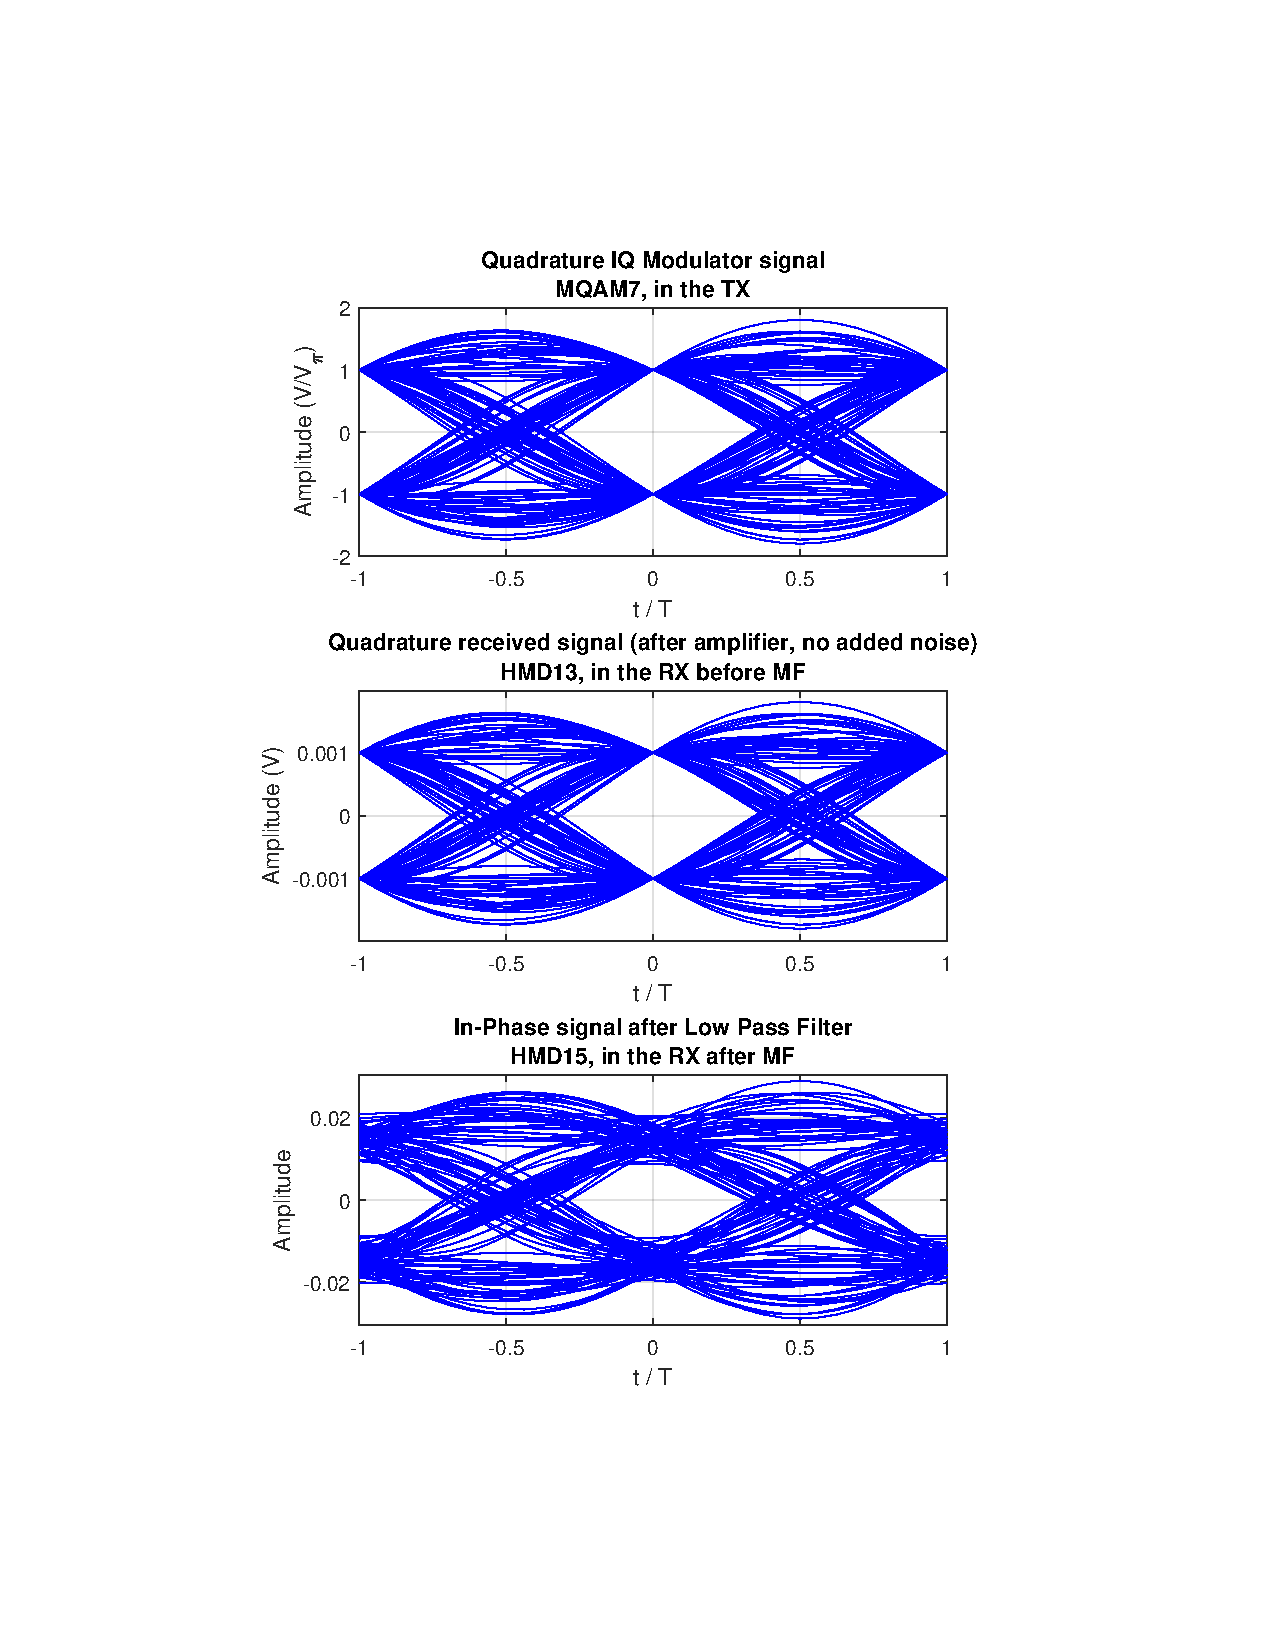
\includegraphics[clip, trim=4cm 4cm 4cm 4cm,
			width=\textwidth]{./sdf/m_qam_system/figures/eyes/simulRc03Sp60Np00_q.pdf}
	\end{subfigure}
	
	\caption{
%		Eye diagrams using matched filtering with raised-cosine without AWGN.
		Obtained at
		three different points in the system: optical output of transmitter on the top;
		the amplified signal at the middle; and
		after the receiver filter.
%		Simulation done with an optical power output of
%		-60~dBm, 0~dBm at the local oscillator, a gain of $10^3$ at the amplifier, and
%		a rolloff factor of 0.3.
		\label{fig:eyes_nn_rc_03}}
	\end{minipage}
\end{figure}

\begin{table}[H]
	\centering
	
	\begin{tabular}{|l|l|}
		\hline
		\multicolumn{2}{|c|}{ \textbf{Simulation Parameters} } \\
		\hline
		\textbf{Parameter}     & \textbf{Default Value}                                     \\\hline
		%		numberOfBitsGenerated  & $40000$	                                                \\\hline
		bitPeriod              & $1/32\times10^9$~s														\\\hline
		%		symbolRate		       &                                                     		\\\hline
		samplesPerSymbol       & $16$                                                       \\\hline
		%		symbolRate		       &                                                     		\\\hline
		%		pLength                & $5$                                                        \\\hline
		%		iqAmplitudesValues     & $\lbrace~\lbrace-1,~0\rbrace~,~\lbrace1,~0\rbrace~\rbrace$ \\\hline
		outputOpticalPower     & $-60$~dBm 													\\ \hline
		shaperFilter	       & RootRaisedCosine												\\ \hline
		outputFilter		   & RootRaisedCosine												\\ \hline
		rollOffFactor		   & 0.3														\\ \hline
		localOscillatorPower   & $0$~dBm                                                    \\ \hline
		localOscillatorPhase   & $0$                                                        \\ \hline
		%		transferMatrix         & $\lbrace~\lbrace \frac{1}{\sqrt{2}},~\frac{1}{\sqrt{2}},~\frac{1}{\sqrt{2}},~\frac{-1}{\sqrt{2}} \rbrace~\rbrace$ & \\ \hline
		responsivity           & $1$                                                        \\ \hline
		amplification          & $10^3$                                                     \\ \hline
		noisePower   & $0$~V$^2$                             					\\ \hline
		%		confidence             & $0.95$                                                     \\ \hline
		%		midReportSize          & $0$                                                        \\ \hline
	\end{tabular}
\end{table}
\begin{figure}[H]
		\centering
	\textbf{Root-Raised-Cosine Signal (roll-off=0.3) with Matched Filtering}
	\begin{minipage}{\linewidth}
		\centering
	\begin{subfigure}{.45\textwidth}
		\centering
		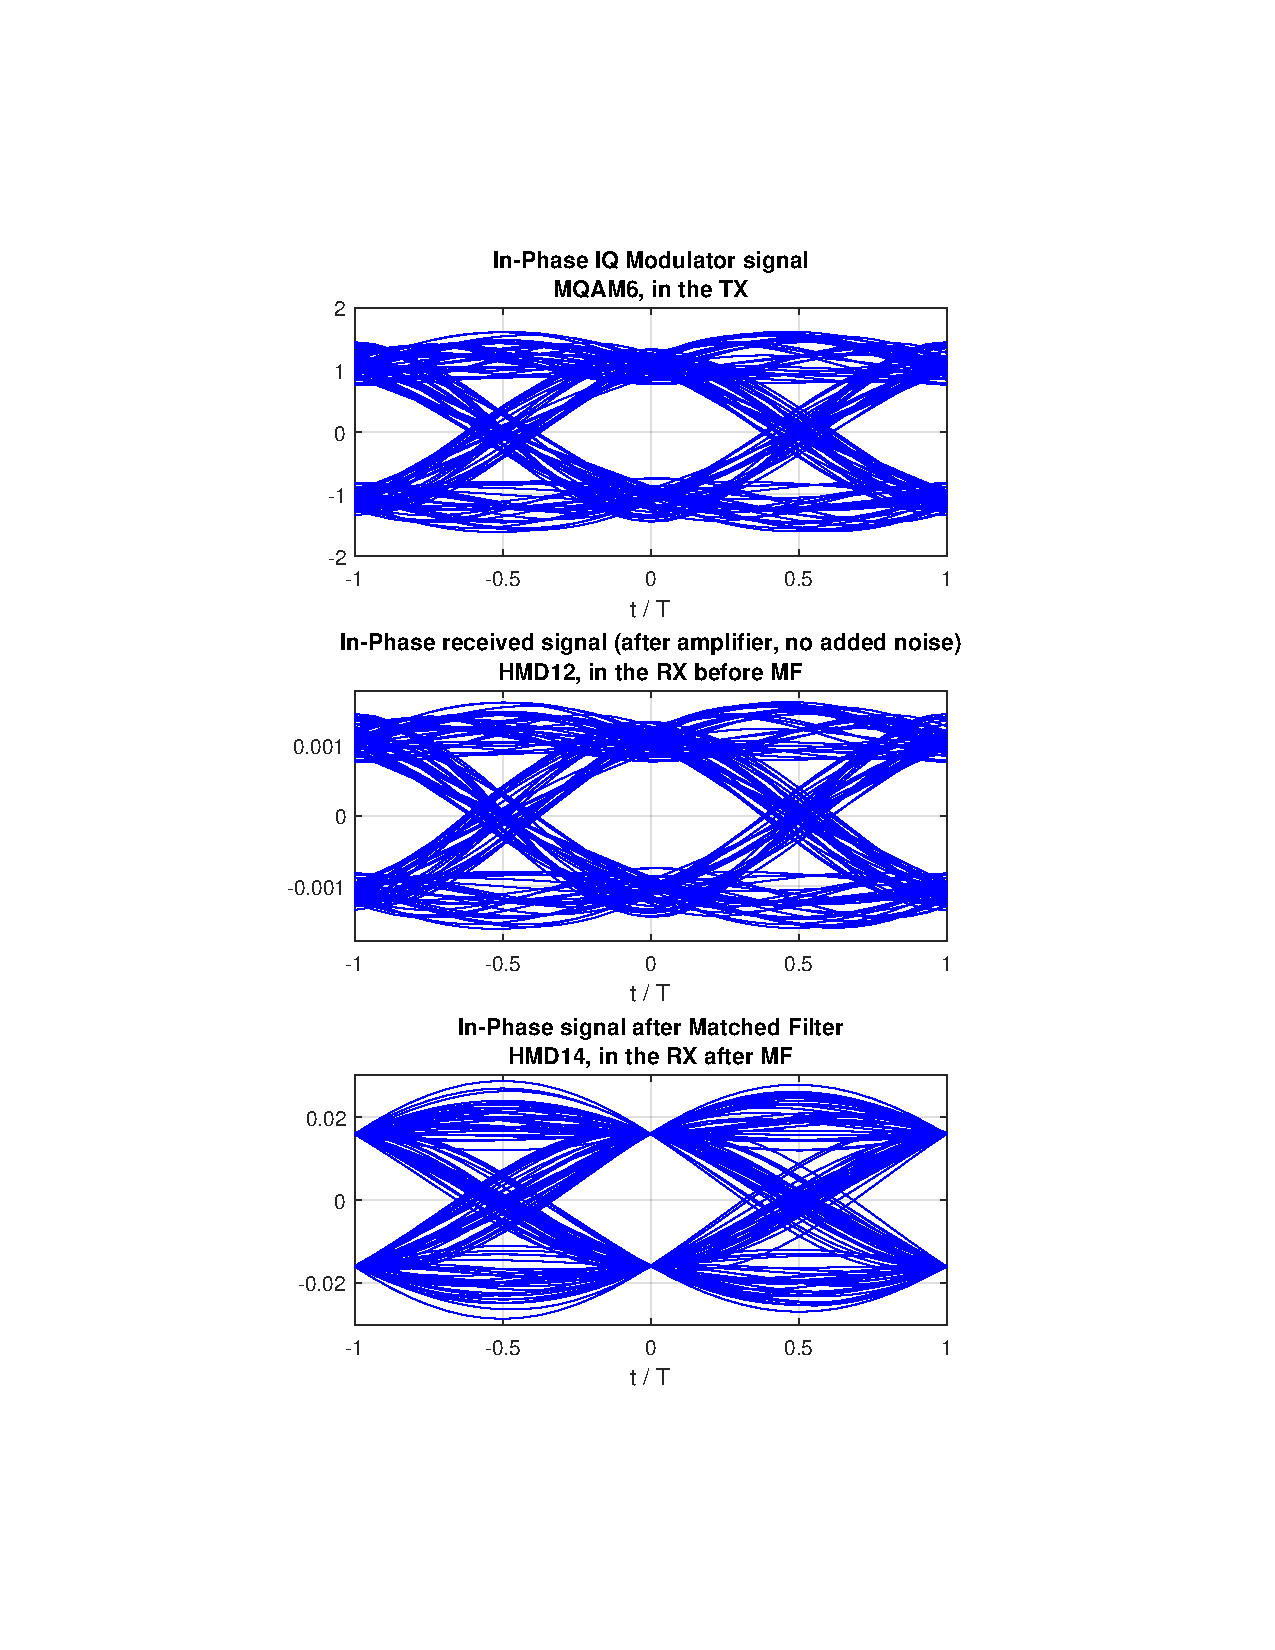
\includegraphics[clip, trim=4cm 4cm 4cm 4cm,
			width=\textwidth]{./sdf/m_qam_system/figures/eyes/simulRrc03Sp60Np00_i.pdf}
	\end{subfigure}
	\begin{subfigure}{.45\textwidth}
		\centering
		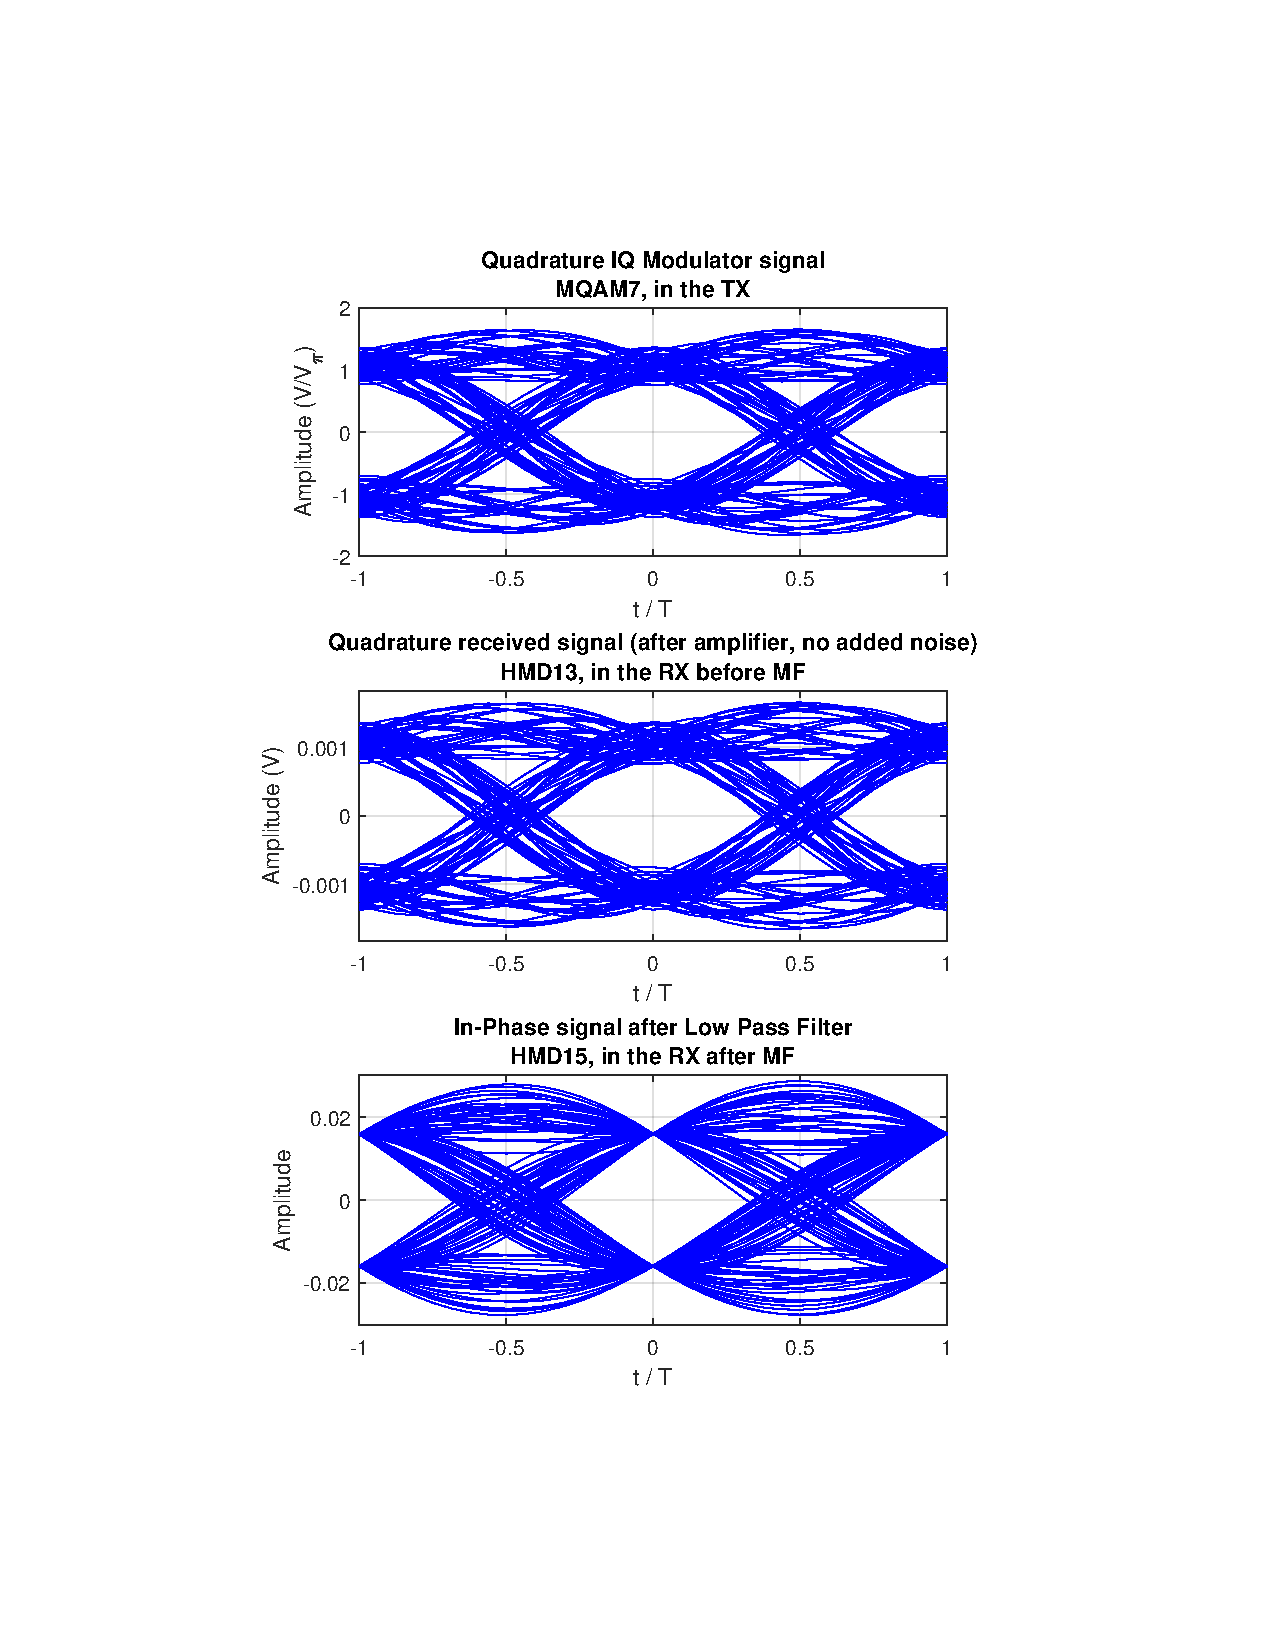
\includegraphics[clip, trim=4cm 4cm 4cm 4cm,
			width=\textwidth]{./sdf/m_qam_system/figures/eyes/simulRrc03Sp60Np00_q.pdf}
	\end{subfigure}
	
	\caption{
%		Eye diagrams using matched filtering with root-raised-cosine without AWGN.
		Obtained at
		three different points in the system: optical output of transmitter on the top;
		the amplified signal at the middle; and
		after the receiver filter.
%		Simulation done with an optical power output
%		of -60~dBm, 0~dBm at the local oscillator, a gain of $10^3$ at the amplifier,
%		and a rolloff factor of 0.3.
		\label{fig:eyes_nn_rrc_03}}
	\end{minipage}
	
\end{figure}

Thus, it can be concluded that, in order to avoid inter-symbol interference,
the filters used should be raised-cosine or root-raised-cosine, if not using a
filter at the receiver or if using matched filtering, respectively. As such,
from now on only these configurations will be used.

\subsubsection{With Noise (High SNR)}

In this section and the following one, a comparison will be presented between
not using a filter on the receiver and using matched filtering. This comparison
will be made for signals affected by added white gaussian noise, where the
noise is added to the signal after the amplifier stage and before the signal
passes through the filter on the receiver.

For the first case, where no filter is present at the receiver, a
raised-cosine filter will be used at the pulse shaper. For matched filtering, a
root-raised-cosine filter will be used at the pulse-shaper and the receiver.

Figures \ref{fig:eyes_n_rc_45_09}-\ref{fig:eyes_n_rrc_45_09} show the eye
diagrams for both these cases. The optical power used was $-45~dBm$, the
noise power was set at $10^{-6} V^2$, and the roll-off factor was set
to $0.9$ in both cases. In both cases, its is still possible to visibly see the
approximate shape of the signal after noise is added, even without matched
filtering. However, it can be seen that the output signal in the case with
matched filtering is much less affected by noise, as the root-raised-cosine at
the receiver is rather effective at filtering the noise.

\begin{table}[H]
	\centering
	
	\begin{tabular}{|l|l|}
		\hline
		\multicolumn{2}{|c|}{ \textbf{Simulation Parameters} } \\
		\hline
		\textbf{Parameter}     & \textbf{Default Value}                                     \\\hline
		%		numberOfBitsGenerated  & $40000$	                                                \\\hline
		bitPeriod              & $1/32\times10^9$~s														\\\hline
		%		symbolRate		       &                                                     		\\\hline
		samplesPerSymbol       & $16$                                                       \\\hline
		%		symbolRate		       &                                                     		\\\hline
		%		pLength                & $5$                                                        \\\hline
		%		iqAmplitudesValues     & $\lbrace~\lbrace-1,~0\rbrace~,~\lbrace1,~0\rbrace~\rbrace$ \\\hline
		outputOpticalPower     & $-45$~dBm 													\\ \hline
		shaperFilter	       & RaisedCosine												\\ \hline
		outputFilter		   & 															\\ \hline
		rollOffFactor		   & 0.9														\\ \hline
		localOscillatorPower   & $0$~dBm                                                    \\ \hline
		localOscillatorPhase   & $0$                                                        \\ \hline
		%		transferMatrix         & $\lbrace~\lbrace \frac{1}{\sqrt{2}},~\frac{1}{\sqrt{2}},~\frac{1}{\sqrt{2}},~\frac{-1}{\sqrt{2}} \rbrace~\rbrace$ & \\ \hline
		responsivity           & $1$                                                        \\ \hline
		amplification          & $10^3$                                                     \\ \hline
		noisePower   & $10^{-6}$~V$^2$                             					\\ \hline
		%		confidence             & $0.95$                                                     \\ \hline
		%		midReportSize          & $0$                                                        \\ \hline
		theoreticalSNR  	   & $15~dB$                             					\\ \hline
		numericalSNR 		   & $13.9182~dB$                             					\\ \hline
		numericalSNR Upper Bound (95\% confidence) & $13.9624~dB$                             					\\ \hline
		numericalSNR Lower Bound (95\% confidence) & $13.8737~dB$                             					\\ \hline
	\end{tabular}
\end{table}
\begin{figure}[H]
		\centering
	\textbf{Raised-Cosine Signal (roll-off=0.9) with Added Noise, SNR = 15 dB}
	\begin{minipage}{\linewidth}
		\centering
	\begin{subfigure}{.45\textwidth}
		\centering
		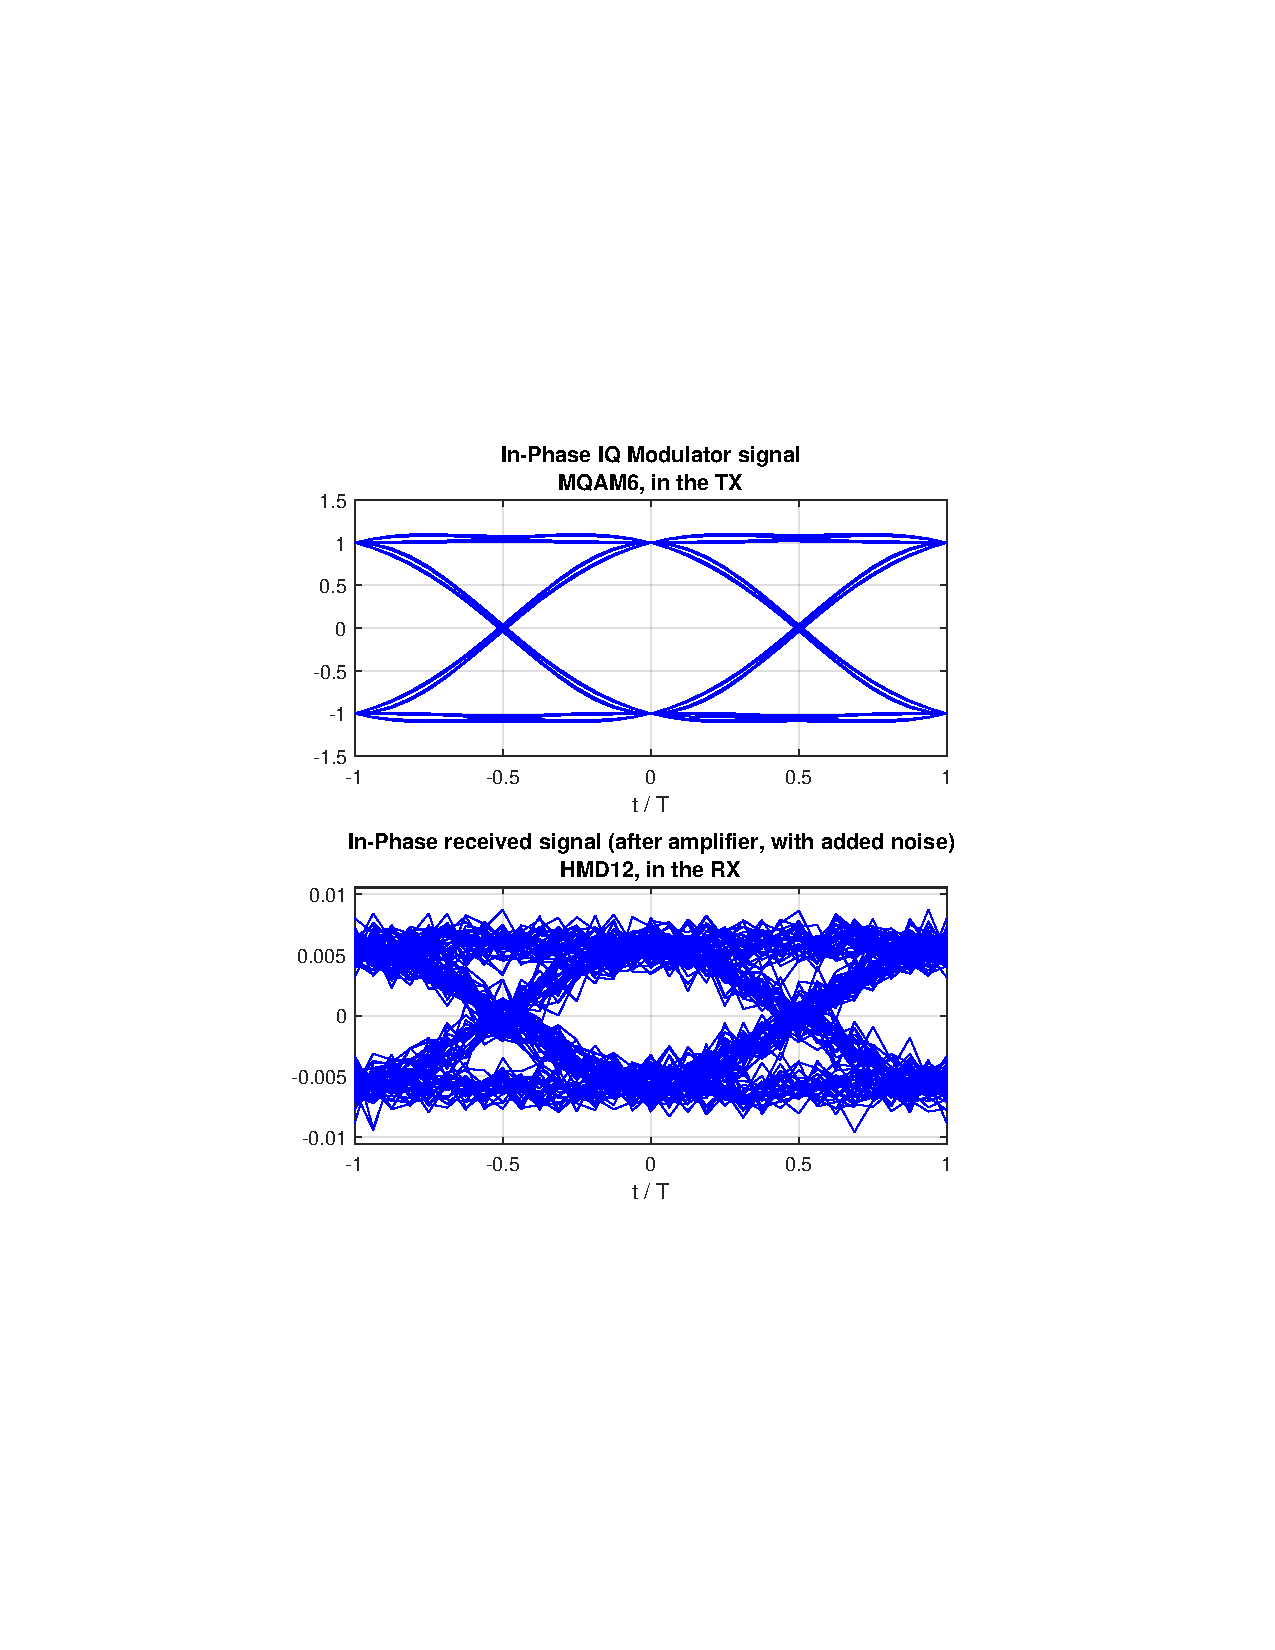
\includegraphics[clip, trim=4cm 7cm 4cm 7cm, 
		width=\textwidth]{./sdf/m_qam_system/figures/eyes/simulRc09Sp45Np60_i.pdf}
	\end{subfigure}
	\begin{subfigure}{.45\textwidth}
		\centering
		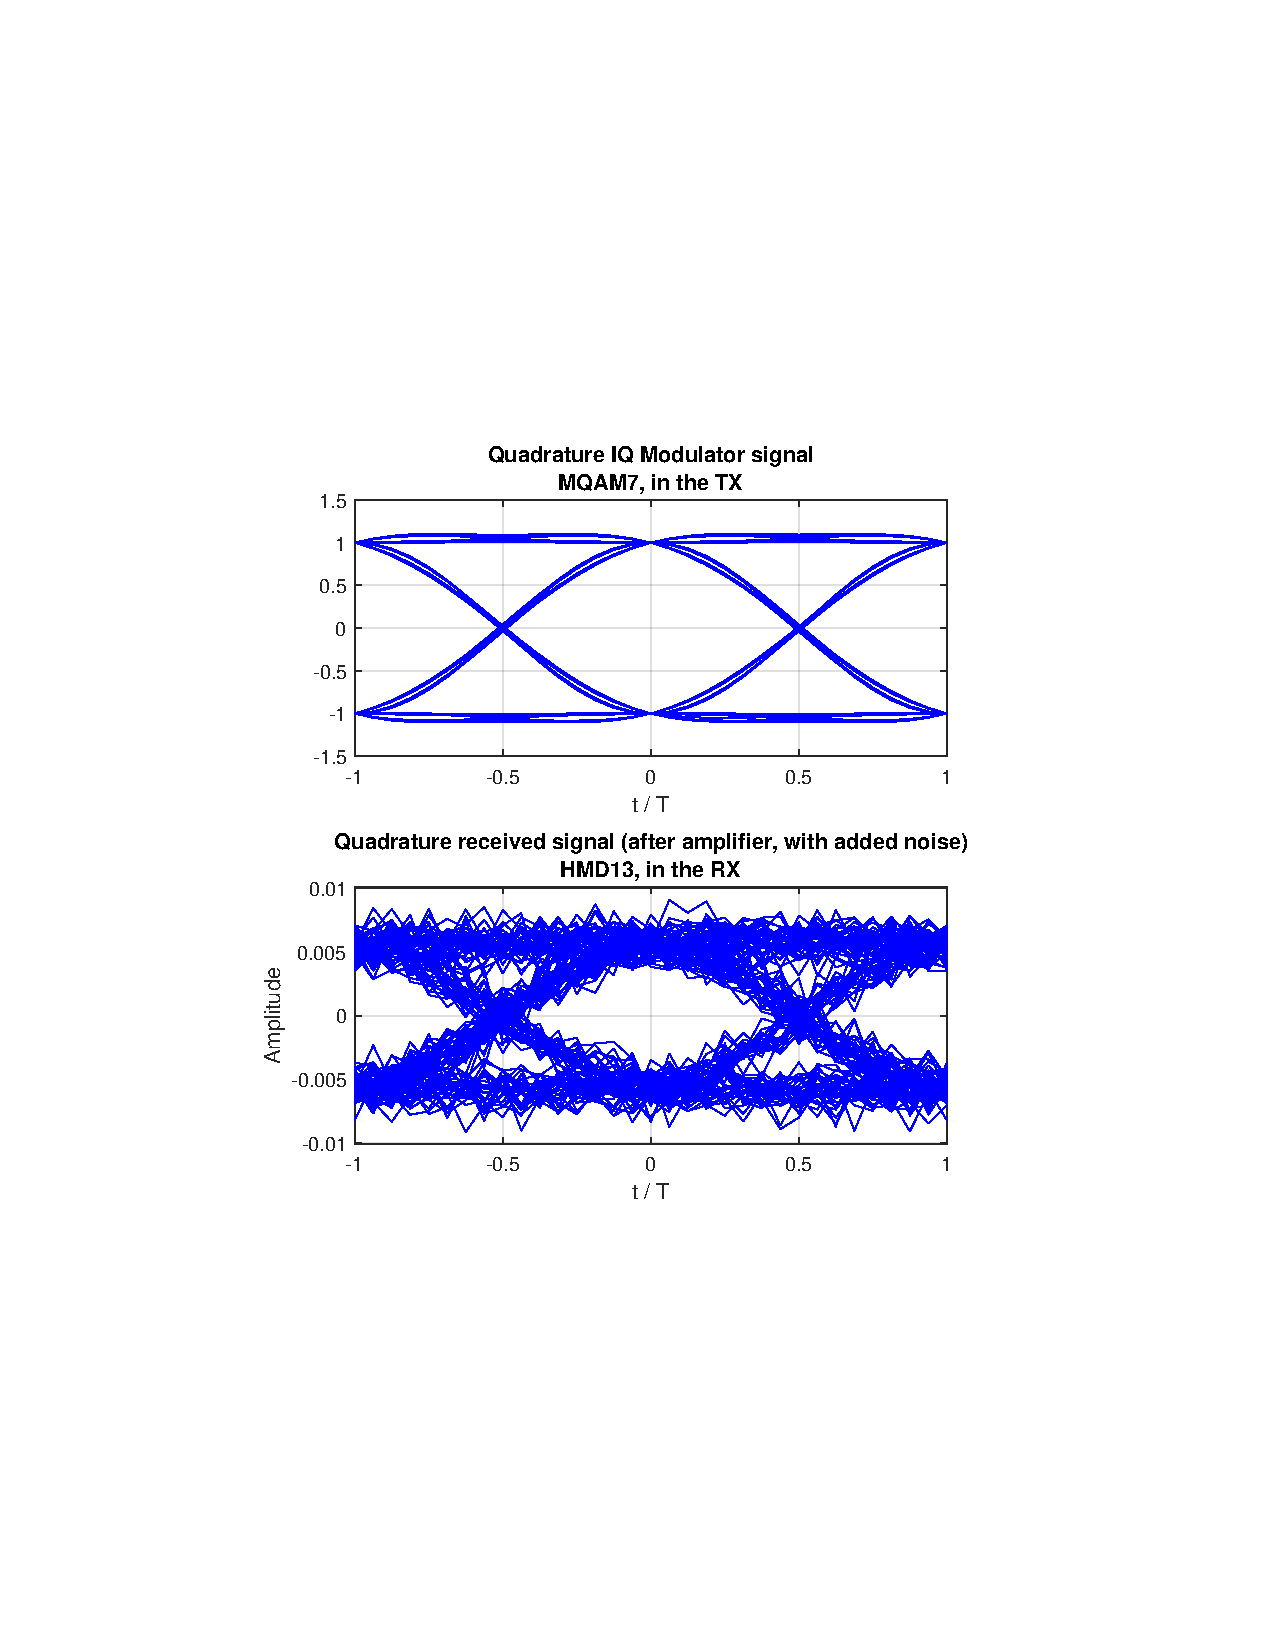
\includegraphics[clip, trim=4cm 7cm 4cm 7cm, 
		width=\textwidth]{./sdf/m_qam_system/figures/eyes/simulRc09Sp45Np60_q.pdf}
	\end{subfigure}
	
	\caption{
%		Eye diagrams without matched filtering using raised-cosine.
		Obtained
		at two different points in the system: optical output of transmitter on the top and
		the noisy signal at the bottom.
%		Obtained through simulation with an optical power output of
%		-45~dBm, 0~dBm at the local oscillator, a gain of $10^3$ at the amplifier, a
%		noise spectral density of $10^{-6}$ and a rolloff factor of
%		0.9.
		\label{fig:eyes_n_rc_45_09}}
	\end{minipage}
\end{figure}
\begin{table}[H]
	\centering
	
	\begin{tabular}{|l|l|}
		\hline
		\multicolumn{2}{|c|}{ \textbf{Simulation Parameters} } \\
		\hline
		\textbf{Parameter}     & \textbf{Default Value}                                     \\\hline
		%		numberOfBitsGenerated  & $40000$	                                                \\\hline
		bitPeriod              & $1/32\times10^9$~s														\\\hline
		%		symbolRate		       &                                                     		\\\hline
		samplesPerSymbol       & $16$                                                       \\\hline
		%		symbolRate		       &                                                     		\\\hline
		%		pLength                & $5$                                                        \\\hline
		%		iqAmplitudesValues     & $\lbrace~\lbrace-1,~0\rbrace~,~\lbrace1,~0\rbrace~\rbrace$ \\\hline
		outputOpticalPower     & $-45$~dBm 													\\ \hline
		shaperFilter	       & RootRaisedCosine												\\ \hline
		outputFilter		   & RootRaisedCosine												\\ \hline
		rollOffFactor		   & 0.9														\\ \hline
		localOscillatorPower   & $0$~dBm                                                    \\ \hline
		localOscillatorPhase   & $0$                                                        \\ \hline
		%		transferMatrix         & $\lbrace~\lbrace \frac{1}{\sqrt{2}},~\frac{1}{\sqrt{2}},~\frac{1}{\sqrt{2}},~\frac{-1}{\sqrt{2}} \rbrace~\rbrace$ & \\ \hline
		responsivity           & $1$                                                        \\ \hline
		amplification          & $10^3$                                                     \\ \hline
		noisePower   & $10^{-6}$~V$^2$                             					\\ \hline
		theoreticalSNR  	   & $15~dB$                             					\\ \hline
		numericalSNR 		     & $14.9902~dB$                             					\\ \hline
		numericalSNR Upper Bound (95\% confidence) & $15.0408~dB$                             					\\ \hline
		numericalSNR Lower Bound (95\% confidence) & $14.9391~dB$                             					\\ \hline
		%		confidence             & $0.95$                                                     \\ \hline
		%		midReportSize          & $0$                                                        \\ \hline
	\end{tabular}
\end{table}
\begin{figure}[H]
	\centering
\textbf{Root-Raised-Cosine Signal (roll-off=0.9) with Added Noise and Matched Filtering,\\SNR = 15}
\begin{minipage}{\linewidth}
	\centering
	\begin{subfigure}{.45\textwidth}
		\centering
			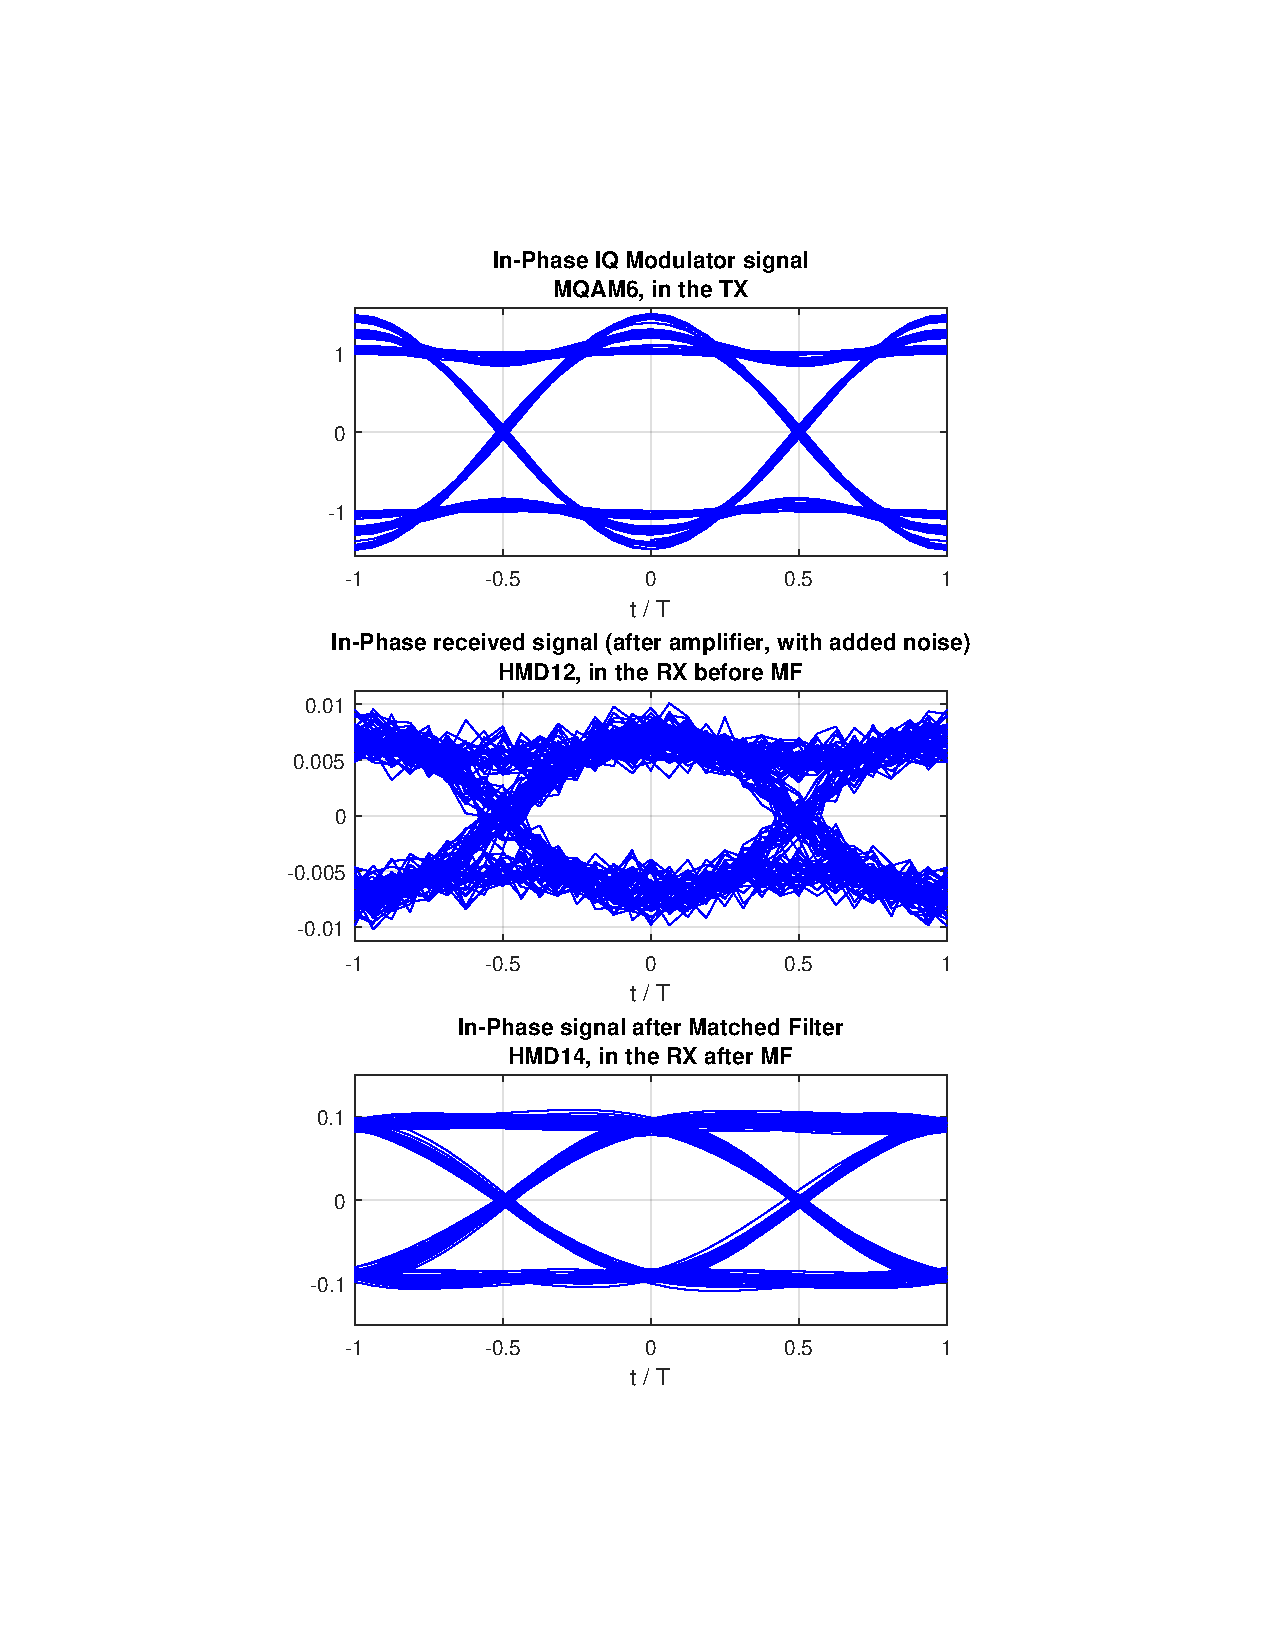
\includegraphics[clip, trim=4cm 4cm 4cm 4cm, 
			width=\textwidth]{./sdf/m_qam_system/figures/eyes/simulRrc09Sp45Np60_i.pdf}
	\end{subfigure}
	\begin{subfigure}{.45\textwidth}
		\centering
		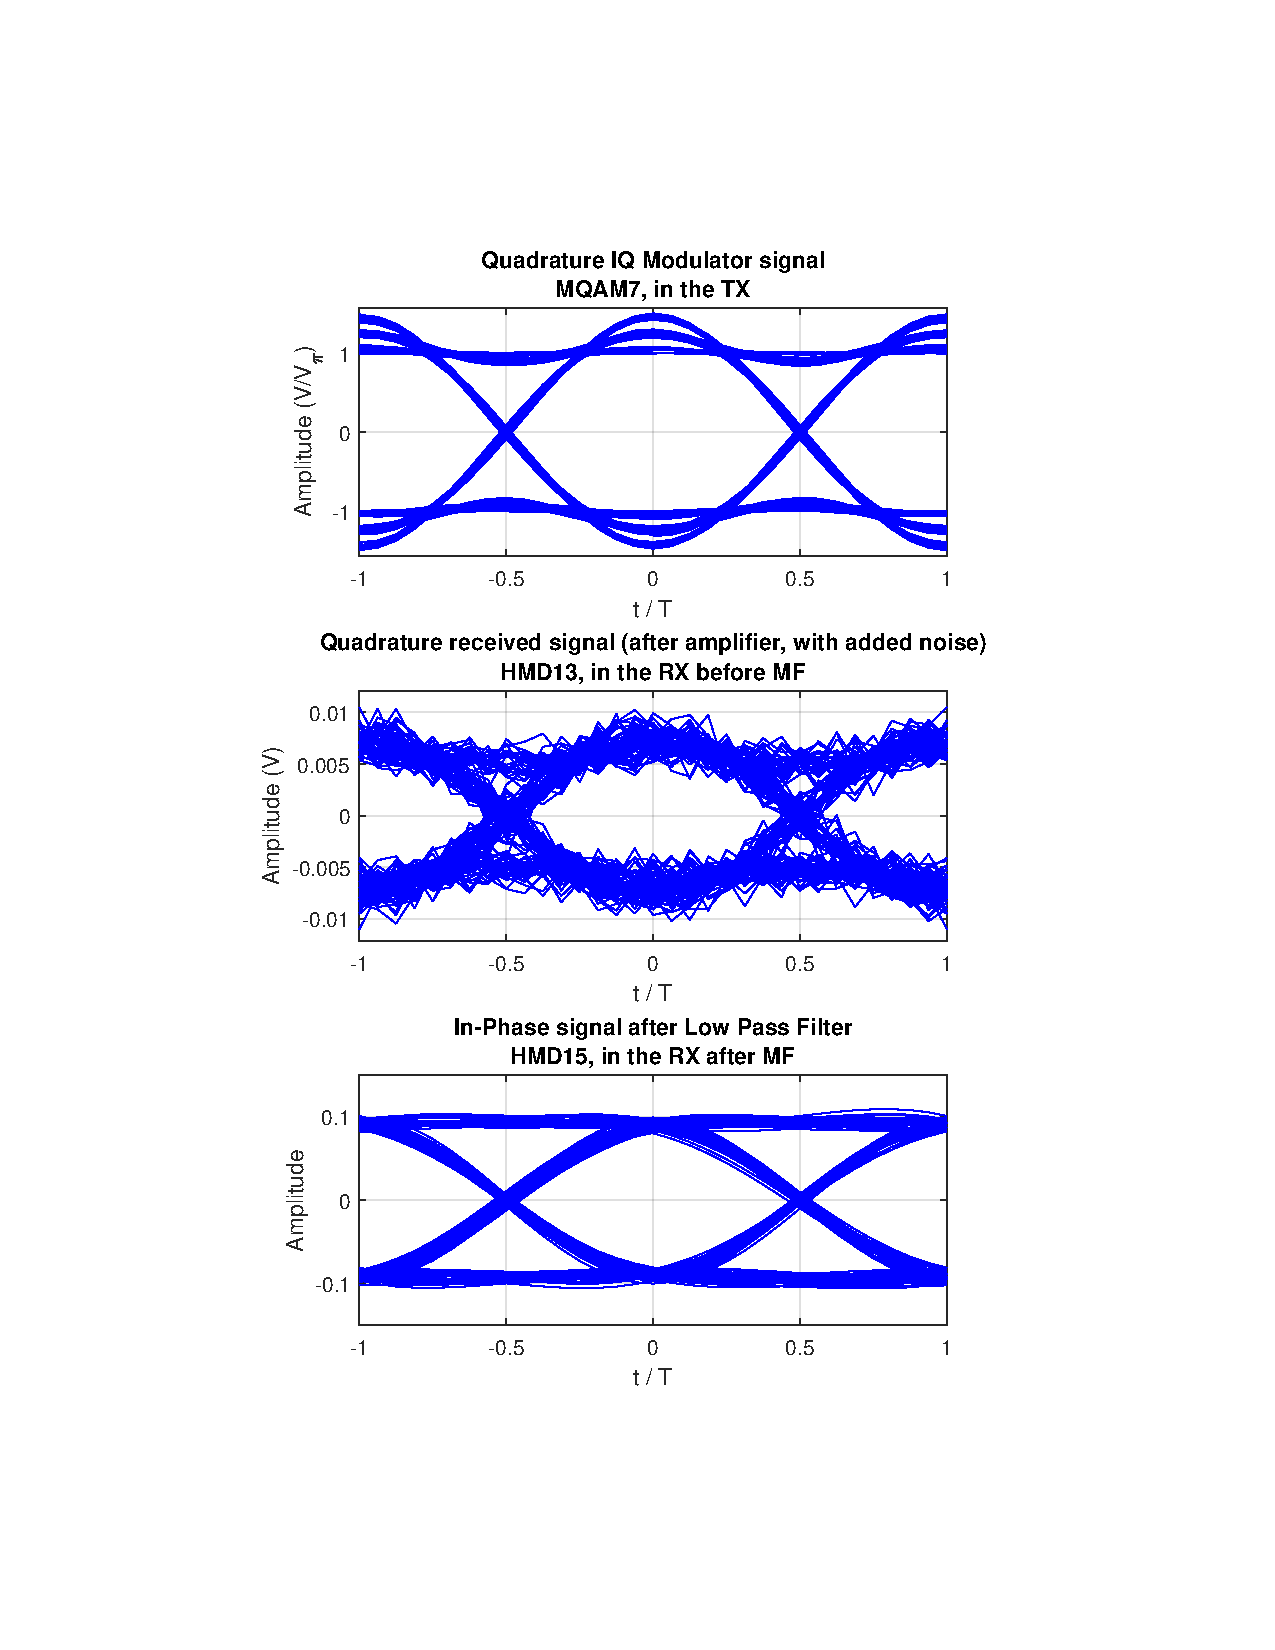
\includegraphics[clip, trim=4cm 4cm 4cm 4cm, 
		width=\textwidth]{./sdf/m_qam_system/figures/eyes/simulRrc09Sp45Np60_q.pdf}
	\end{subfigure}
	
	\caption{
%		Eye diagrams using matched filtering with root-raised-cosine.
		Obtained at three different points in the system: optical output of transmitter on the top;
		the amplified signal at the middle; and
		after the receiver filter.
%		Simulation done with an optical
%		power output of -45~dBm, 0~dBm at the local oscillator, a gain of $10^3$ at the
%		amplifier, a noise spectral density of $10^{-6}$ and a rolloff factor of
%		0.9.
		\label{fig:eyes_n_rrc_45_09}}
	\end{minipage}
\end{figure}


Figures~\ref{fig:eyes_n_rc_45_03} and~\ref{fig:eyes_n_rrc_45_03} show the
cases described above, but with a roll-off factor of 0.3. It can be seen that
the case is in all aspects similar to the one presented above.

\begin{table}[H]
	\centering
	
	\begin{tabular}{|l|l|}
		\hline
		\multicolumn{2}{|c|}{ \textbf{Simulation Parameters} } \\
		\hline
		\textbf{Parameter}     & \textbf{Default Value}                                     \\\hline
		%		numberOfBitsGenerated  & $40000$	                                                \\\hline
		bitPeriod              & $1/32\times10^9$~s														\\\hline
		%		symbolRate		       &                                                     		\\\hline
		samplesPerSymbol       & $16$                                                       \\\hline
		%		symbolRate		       &                                                     		\\\hline
		%		pLength                & $5$                                                        \\\hline
		%		iqAmplitudesValues     & $\lbrace~\lbrace-1,~0\rbrace~,~\lbrace1,~0\rbrace~\rbrace$ \\\hline
		outputOpticalPower     & $-45$~dBm 													\\ \hline
		shaperFilter	       & RaisedCosine												\\ \hline
		outputFilter		   &                     										\\ \hline
		rollOffFactor		   & 0.3														\\ \hline
		localOscillatorPower   & $0$~dBm                                                    \\ \hline
		localOscillatorPhase   & $0$                                                        \\ \hline
		%		transferMatrix         & $\lbrace~\lbrace \frac{1}{\sqrt{2}},~\frac{1}{\sqrt{2}},~\frac{1}{\sqrt{2}},~\frac{-1}{\sqrt{2}} \rbrace~\rbrace$ & \\ \hline
		responsivity           & $1$                                                        \\ \hline
		amplification          & $10^3$                                                     \\ \hline
		noisePower   & $10^{-6}$~V$^2$                             					\\ \hline
		theoreticalSNR  	   & $15~dB$                             					\\ \hline
				numericalSNR 		     & $14.6827~dB$                             					\\ \hline
		numericalSNR Upper Bound (95\% confidence) & $14.7321~dB$                             					\\ \hline
		numericalSNR Lower Bound (95\% confidence) & $14.6327~dB$                             					\\ \hline
		%		confidence             & $0.95$                                                     \\ \hline
		%		midReportSize          & $0$                                                        \\ \hline
	\end{tabular}
\end{table}
\begin{figure}[H]
		\centering
	\textbf{Raised-Cosine Signal (roll-off=0.3) with Added Noise, SNR = 15 dB}
	\begin{minipage}{\linewidth}
		\centering
	\begin{subfigure}{.45\textwidth}
		\centering
		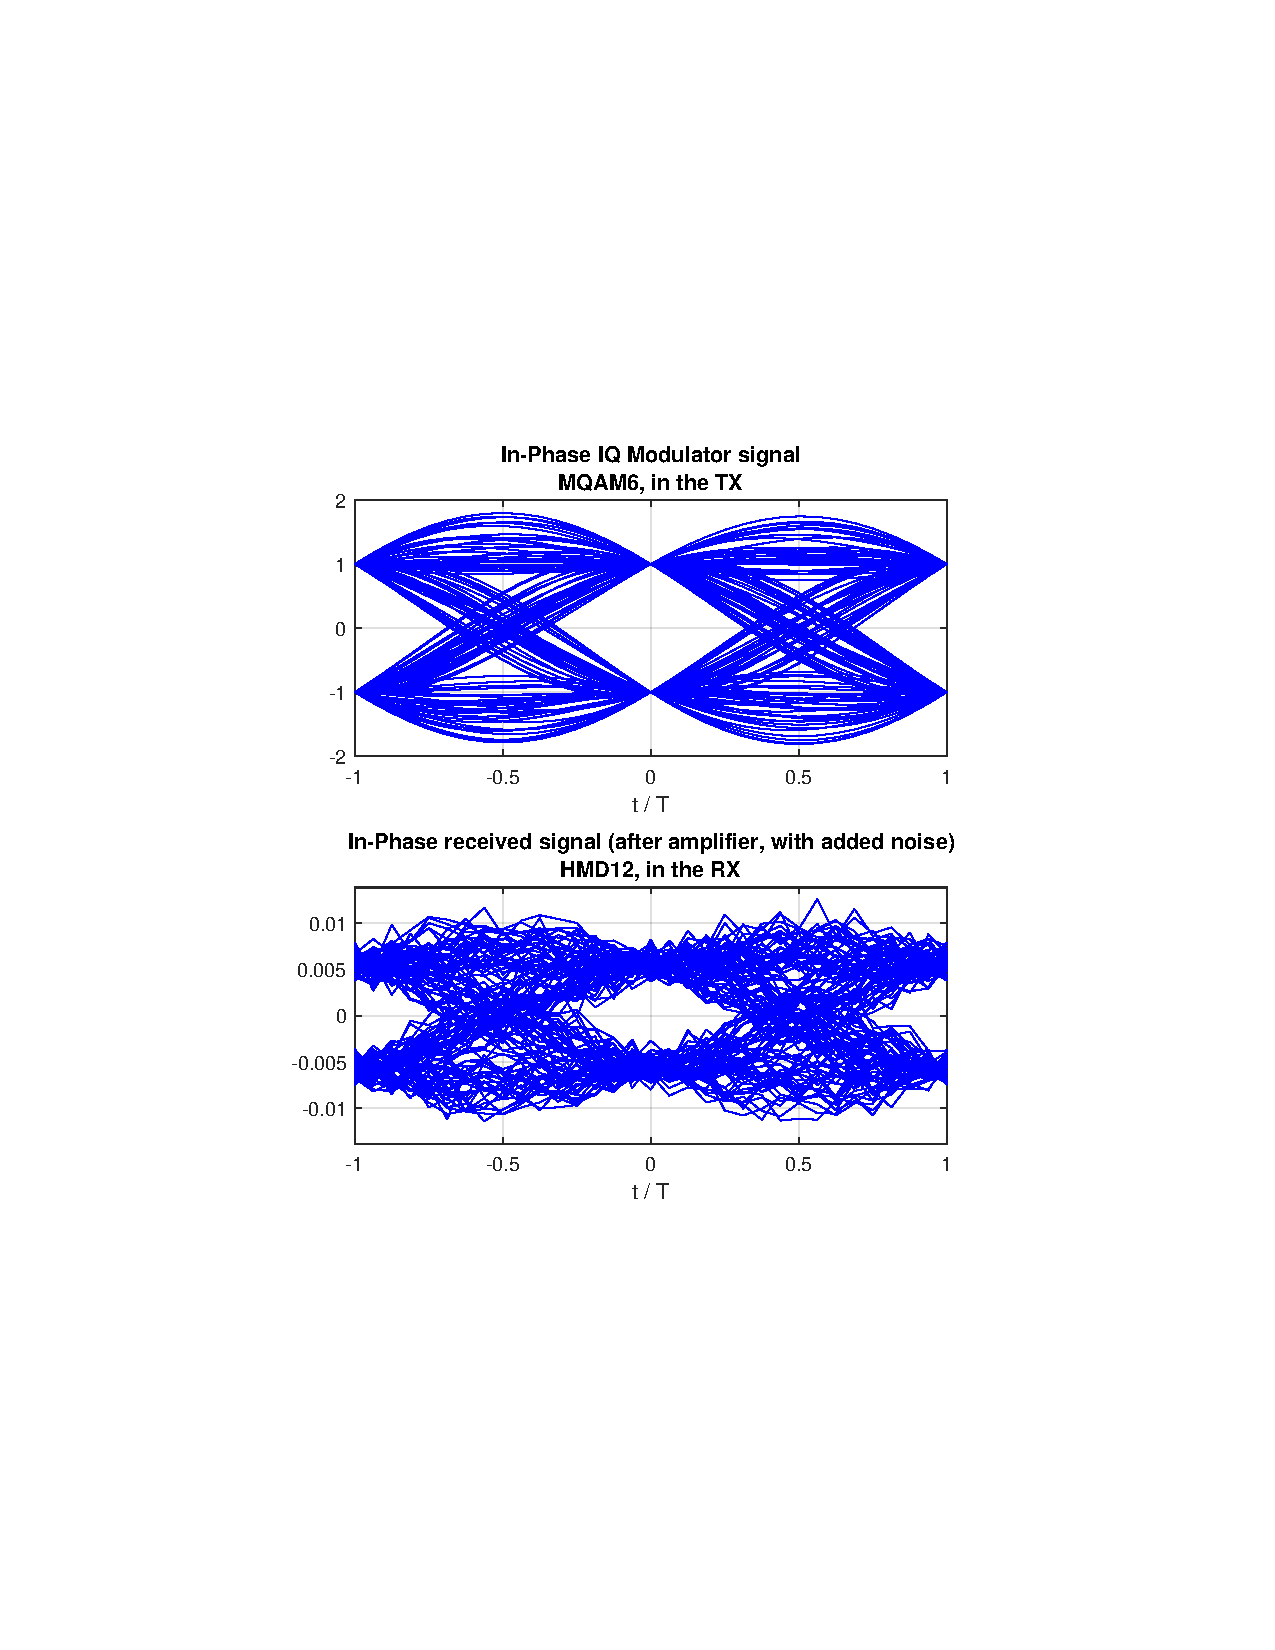
\includegraphics[clip, trim=4cm 7cm 4cm 7cm, 
		width=\textwidth]{./sdf/m_qam_system/figures/eyes/simulRc03Sp45Np60_i.pdf}
	\end{subfigure}
	\begin{subfigure}{.45\textwidth}
		\centering
		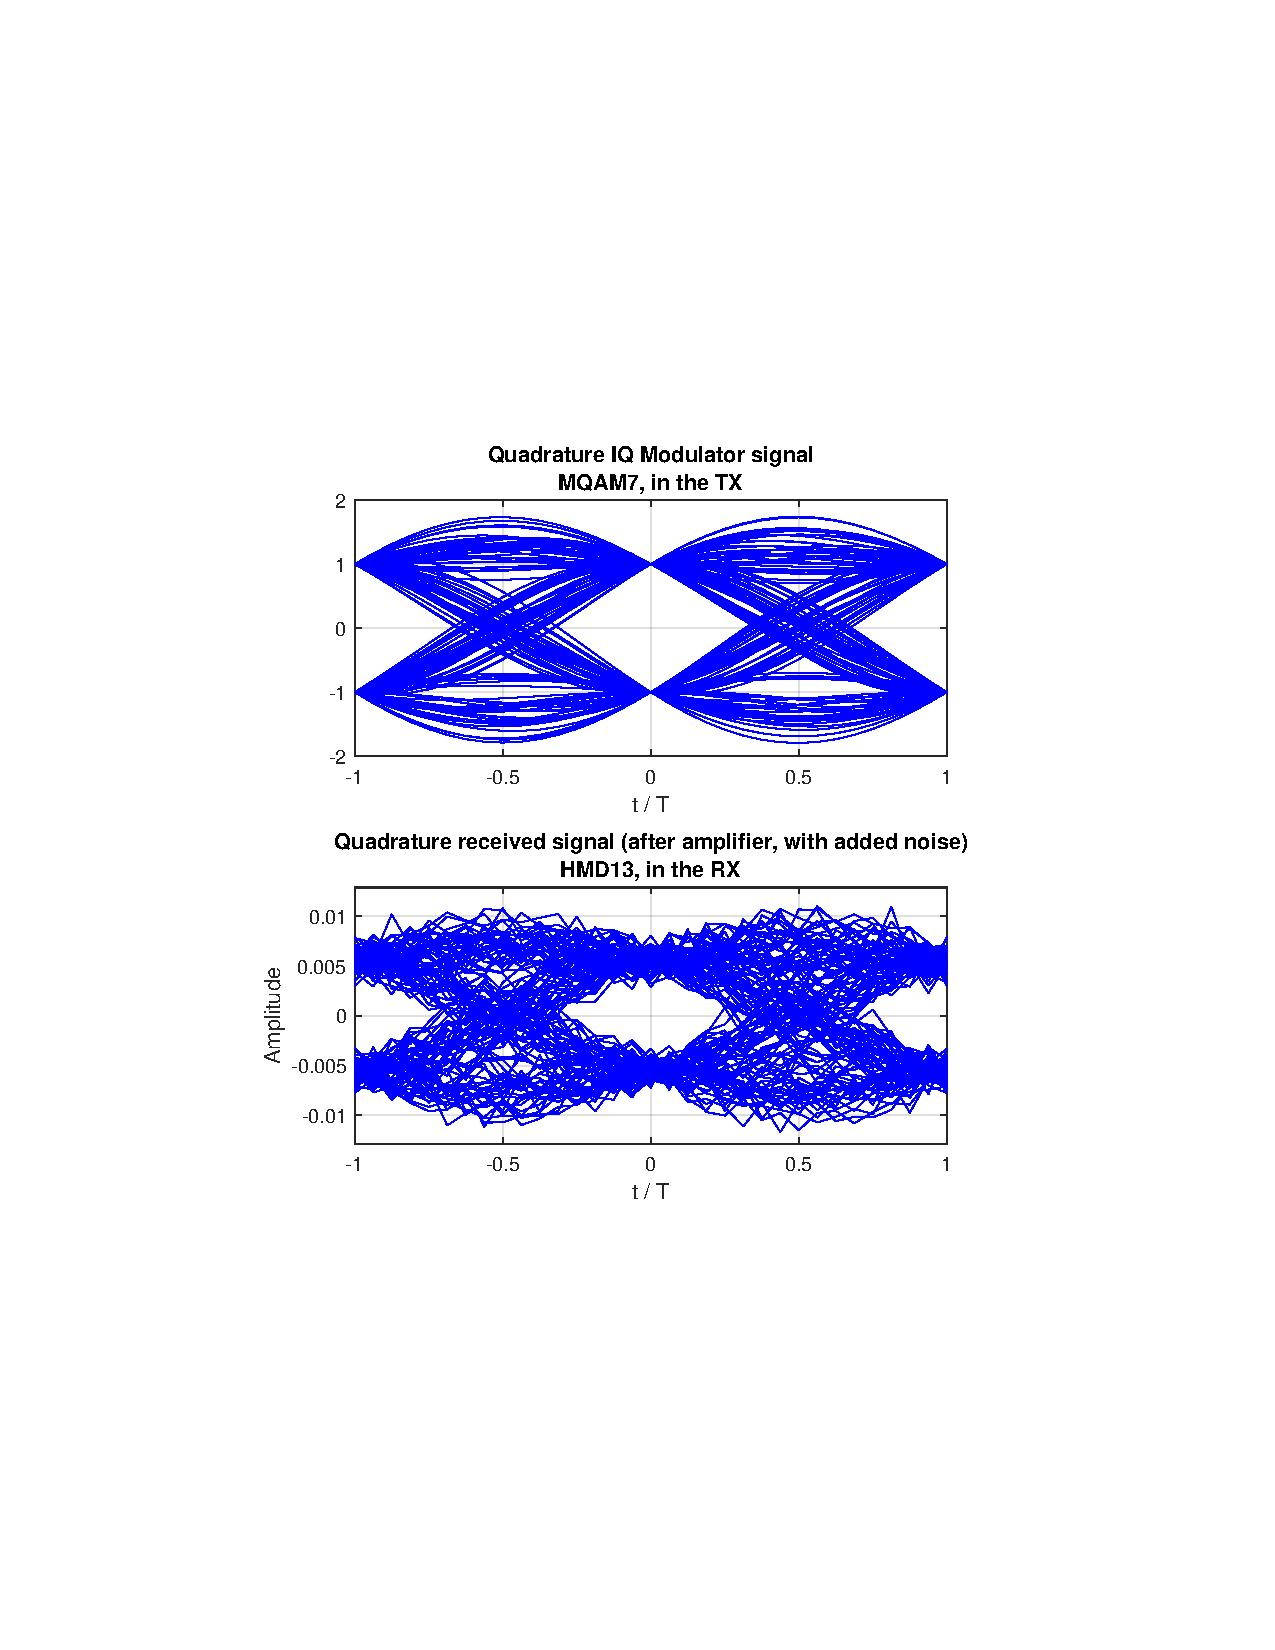
\includegraphics[clip, trim=4cm 7cm 4cm 7cm, 
		width=\textwidth]{./sdf/m_qam_system/figures/eyes/simulRc03Sp45Np60_q.pdf}
	\end{subfigure}
	
	\caption{
%		Eye diagrams without matched filtering with raised-cosine.
		Obtained
		at two different points in the system: optical output of transmitter on the top and
		the noisy signal at the bottom.
%		Simulation done with an optical power output of
%		-45~dBm, 0~dBm at the local oscillator, a gain of $10^3$ at the amplifier, a
%		noise spectral density of $10^{-6}$ and a rolloff factor of
%		0.3.
		\label{fig:eyes_n_rc_45_03}}
	\end{minipage}
\end{figure}
\begin{table}[H]
	\centering
	
	\begin{tabular}{|l|l|}
		\hline
		\multicolumn{2}{|c|}{ \textbf{Simulation Parameters} } \\
		\hline
		\textbf{Parameter}     & \textbf{Default Value}                                     \\\hline
		%		numberOfBitsGenerated  & $40000$	                                                \\\hline
		bitPeriod              & $1/32\times10^9$~s														\\\hline
		%		symbolRate		       &                                                     		\\\hline
		samplesPerSymbol       & $16$                                                       \\\hline
		%		symbolRate		       &                                                     		\\\hline
		%		pLength                & $5$                                                        \\\hline
		%		iqAmplitudesValues     & $\lbrace~\lbrace-1,~0\rbrace~,~\lbrace1,~0\rbrace~\rbrace$ \\\hline
		outputOpticalPower     & $-45$~dBm 													\\ \hline
		shaperFilter	       & RootRaisedCosine												\\ \hline
		outputFilter		   & RootRaisedCosine												\\ \hline
		rollOffFactor		   & 0.3														\\ \hline
		localOscillatorPower   & $0$~dBm                                                    \\ \hline
		localOscillatorPhase   & $0$                                                        \\ \hline
		%		transferMatrix         & $\lbrace~\lbrace \frac{1}{\sqrt{2}},~\frac{1}{\sqrt{2}},~\frac{1}{\sqrt{2}},~\frac{-1}{\sqrt{2}} \rbrace~\rbrace$ & \\ \hline
		responsivity           & $1$                                                        \\ \hline
		amplification          & $10^3$                                                     \\ \hline
		noisePower   & $10^{-6}$~V$^2$                             					\\ \hline
		theoreticalSNR  	   & $15~dB$                             					\\ \hline
		numericalSNR 		     & $14.9696~dB$                             					\\ \hline
		numericalSNR Upper Bound (95\% confidence) & $15.006~dB$                             					\\ \hline
		numericalSNR Lower Bound (95\% confidence) & $14.9329~dB$                             					\\ \hline
		%		confidence             & $0.95$                                                     \\ \hline
		%		midReportSize          & $0$                                                        \\ \hline
	\end{tabular}
\end{table}
\begin{figure}[H]
		\centering
	\textbf{Root-Raised-Cosine Signal (roll-off=0.3) with Added Noise and Matched Filtering, SNR = 15 dB}
	\begin{minipage}{\linewidth}
		\centering
	\begin{subfigure}{.45\textwidth}
		\centering
		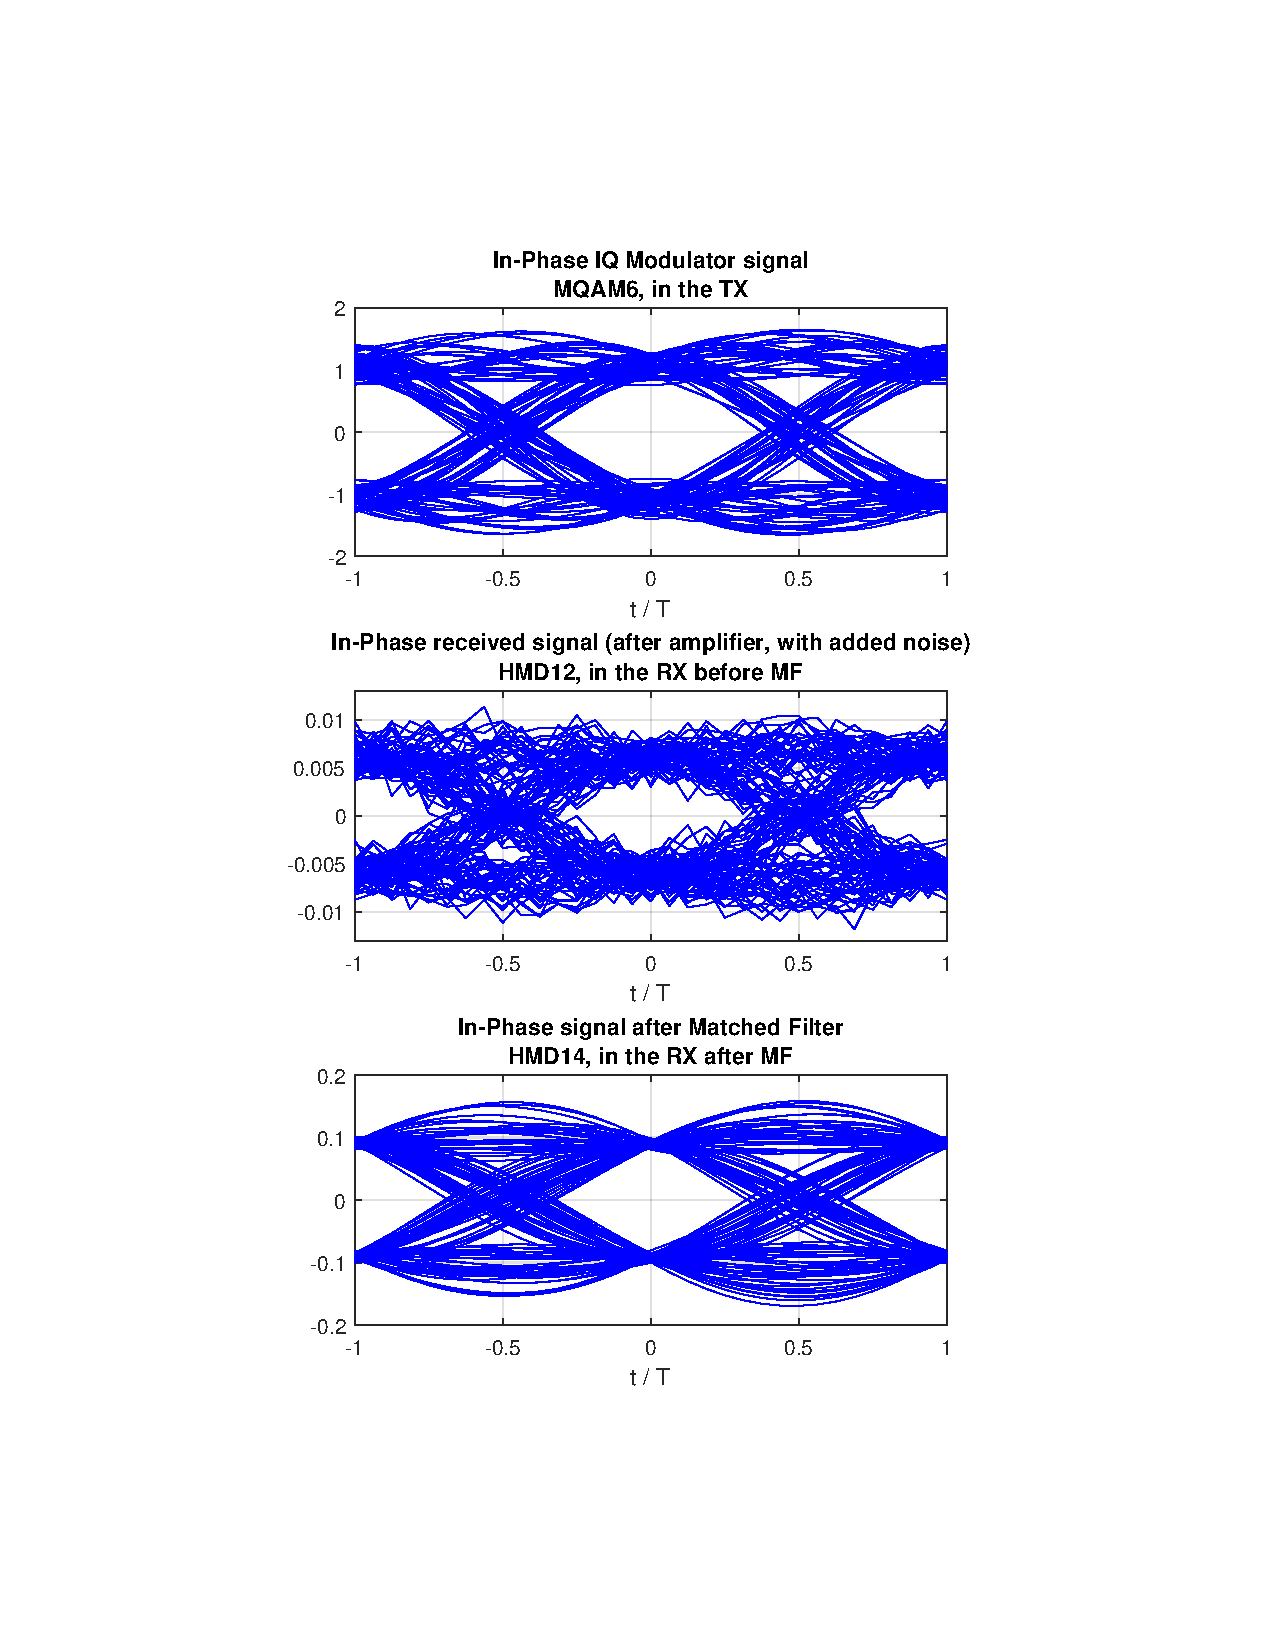
\includegraphics[clip, trim=4cm 4cm 4cm 4cm, 
		width=\textwidth]{./sdf/m_qam_system/figures/eyes/simulRrc03Sp45Np60_i.pdf}
	\end{subfigure}
	\begin{subfigure}{.45\textwidth}
		\centering
		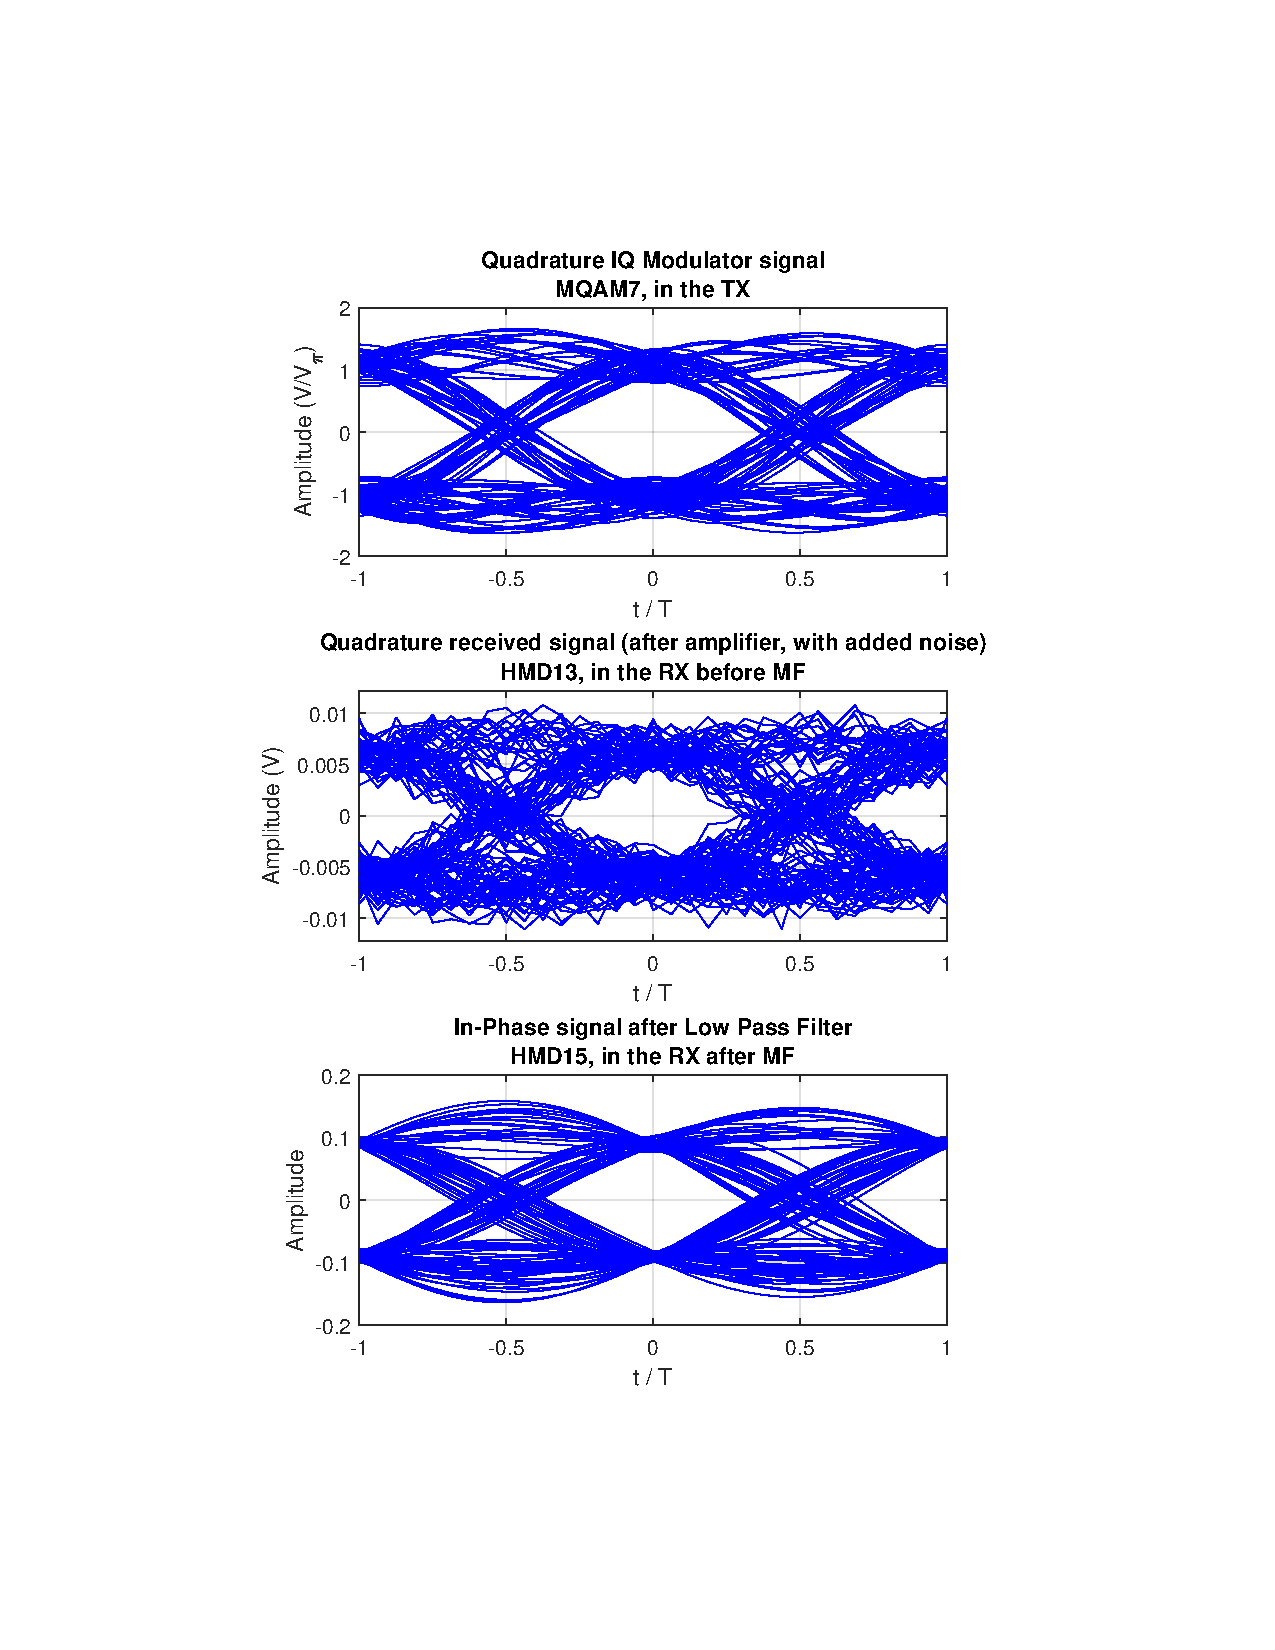
\includegraphics[clip, trim=4cm 4cm 4cm 4cm, 
		width=\textwidth]{./sdf/m_qam_system/figures/eyes/simulRrc03Sp45Np60_q.pdf}
	\end{subfigure}
	
	\caption{
%		Eye diagrams using matched filtering with root-raised-cosine.
		Obtained at three different points in the system: optical output of transmitter on the top;
		the amplified signal at the middle; and
		after the receiver filter.
%		Obtained through simulation with an optical
%		power output of -45~dBm, 0~dBm at the local oscillator, a gain of $10^3$ at the
%		amplifier, a noise spectral density of $10^{-6}$ and a rolloff factor of
%		0.3.
		\label{fig:eyes_n_rrc_45_03}}
	\end{minipage}
\end{figure}



\subsubsection{With Noise (Low SNR)}
Figures \ref{fig:eyes_n_rc_60_09}-\ref {fig:eyes_n_rc_60_03} show eye
diagrams similar to the previous section, but with a lower optical power ($-60~dBm$),
comparable to the average noise power ($10^{-6} V^2$).



Figures~\ref{fig:eyes_n_rc_60_09} and~\ref{fig:eyes_n_rrc_60_09} show the
diagrams obtained without matched filtering and with matched filtering,
respectively, both using a roll-off factor of 0.9.

In this example the effects of matched filtering is even more obvious, as
without it the signal visually appears to be random noise.
\begin{table}[H]
	\centering
	
	\begin{tabular}{|l|l|}
		\hline
		\multicolumn{2}{|c|}{ \textbf{Simulation Parameters} } \\
		\hline
		\textbf{Parameter}     & \textbf{Default Value}                                     \\\hline
		%		numberOfBitsGenerated  & $40000$	                                                \\\hline
		bitPeriod              & $1/32\times10^9$~s														\\\hline
		%		symbolRate		       &                                                     		\\\hline
		samplesPerSymbol       & $16$                                                       \\\hline
		%		symbolRate		       &                                                     		\\\hline
		%		pLength                & $5$                                                        \\\hline
		%		iqAmplitudesValues     & $\lbrace~\lbrace-1,~0\rbrace~,~\lbrace1,~0\rbrace~\rbrace$ \\\hline
		outputOpticalPower     & $-60$~dBm 													\\ \hline
		shaperFilter	       & RaisedCosine												\\ \hline
		outputFilter		   &                											\\ \hline
		rollOffFactor		   & 0.9														\\ \hline
		localOscillatorPower   & $0$~dBm                                                    \\ \hline
		localOscillatorPhase   & $0$                                                        \\ \hline
		%		transferMatrix         & $\lbrace~\lbrace \frac{1}{\sqrt{2}},~\frac{1}{\sqrt{2}},~\frac{1}{\sqrt{2}},~\frac{-1}{\sqrt{2}} \rbrace~\rbrace$ & \\ \hline
		responsivity           & $1$                                                        \\ \hline
		amplification          & $10^3$                                                     \\ \hline
		noisePower   & $10^{-6}$~V$^2$                             					\\ \hline
		theoreticalSNR  	   & $0~dB$                             					\\ \hline
		numericalSNR 		     & $-1.07702~dB$                             					\\ \hline
		numericalSNR Upper Bound (95\% confidence) & $-1.0038~dB$                             					\\ \hline
		numericalSNR Lower Bound (95\% confidence) & $-1.1515~dB$                             					\\ \hline
		%		confidence             & $0.95$                                                     \\ \hline
		%		midReportSize          & $0$                                                        \\ \hline
	\end{tabular}
\end{table}
\begin{figure}[H]
		\centering
	\textbf{Raised-Cosine Signal (roll-off=0.9) with Added Noise, SNR = 0~dB}
	\begin{minipage}{\linewidth}
		\centering
	\begin{subfigure}{.45\textwidth}
		\centering
		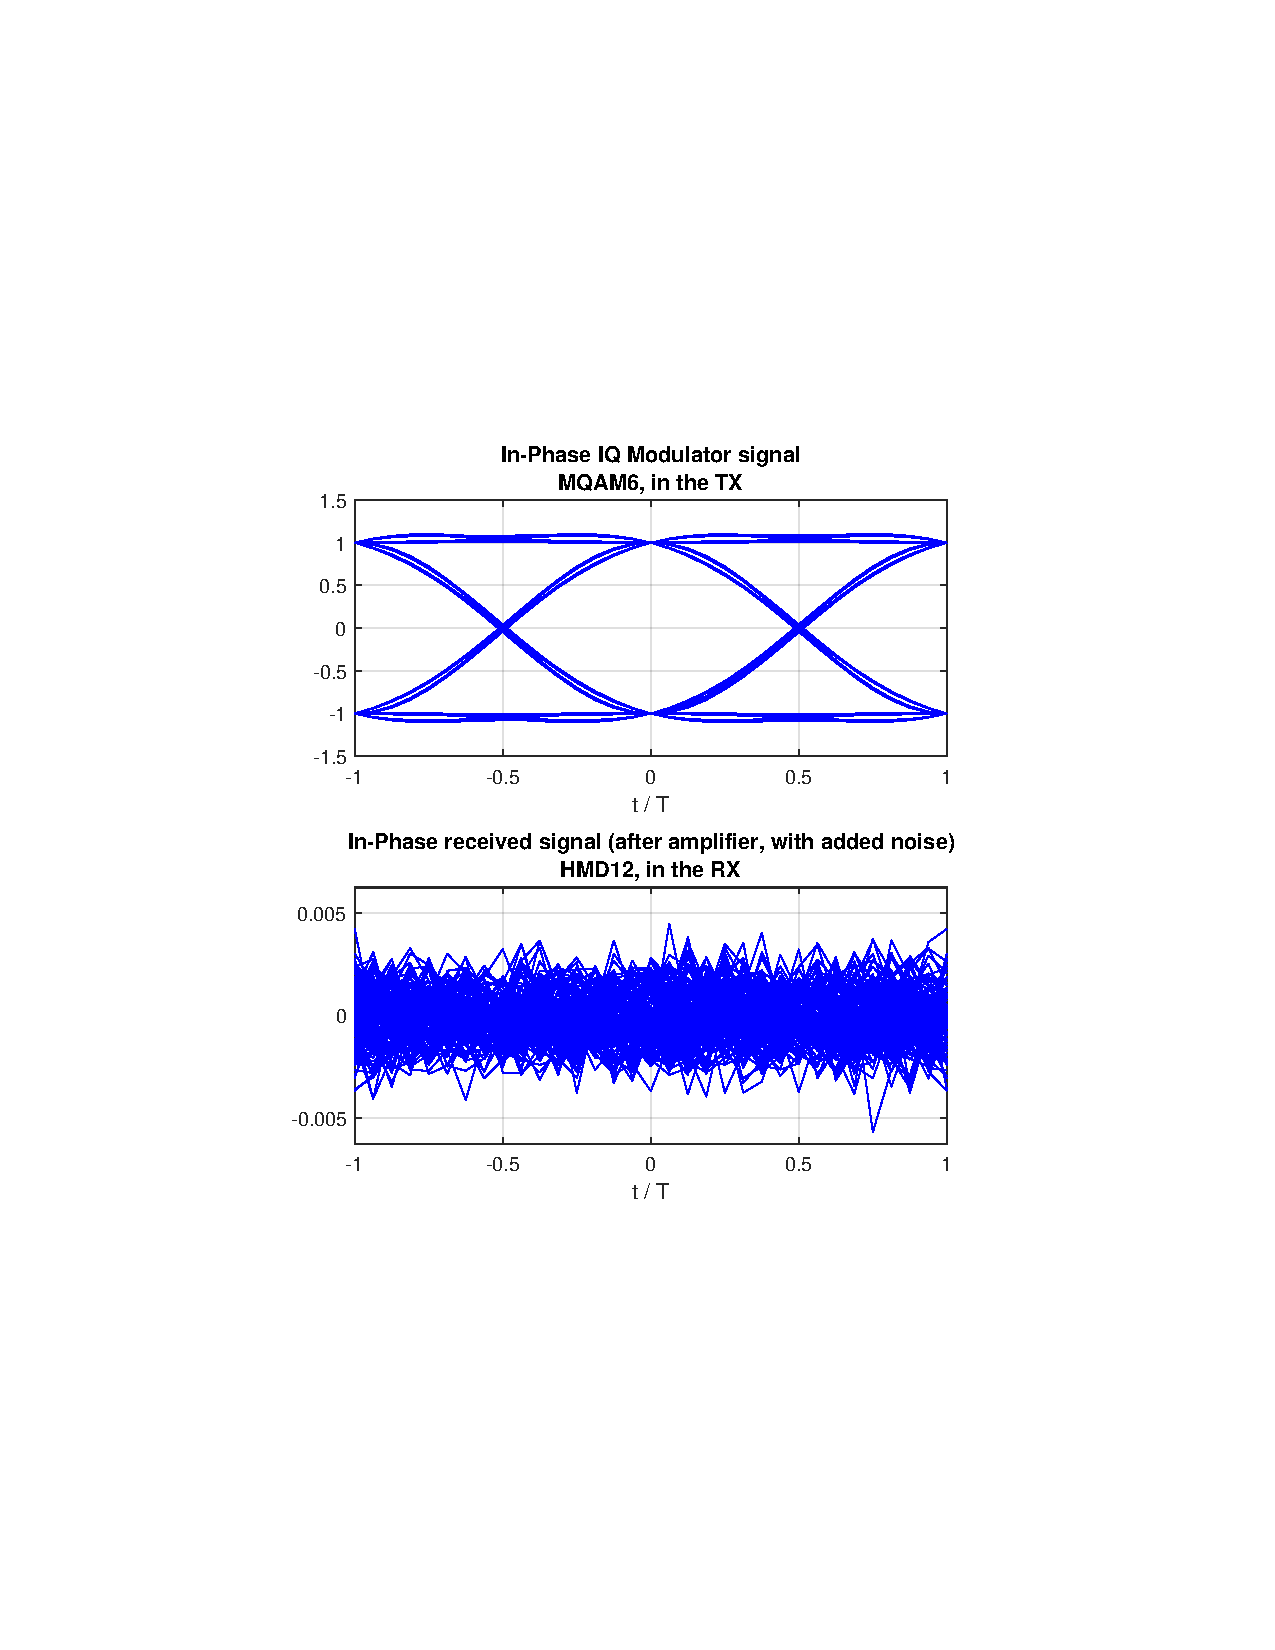
\includegraphics[clip, trim=4cm 7cm 4cm 7cm, 
		width=\textwidth]{./sdf/m_qam_system/figures/eyes/simulRc09Sp60Np60_i.pdf}
	\end{subfigure}
	\begin{subfigure}{.45\textwidth}
		\centering
		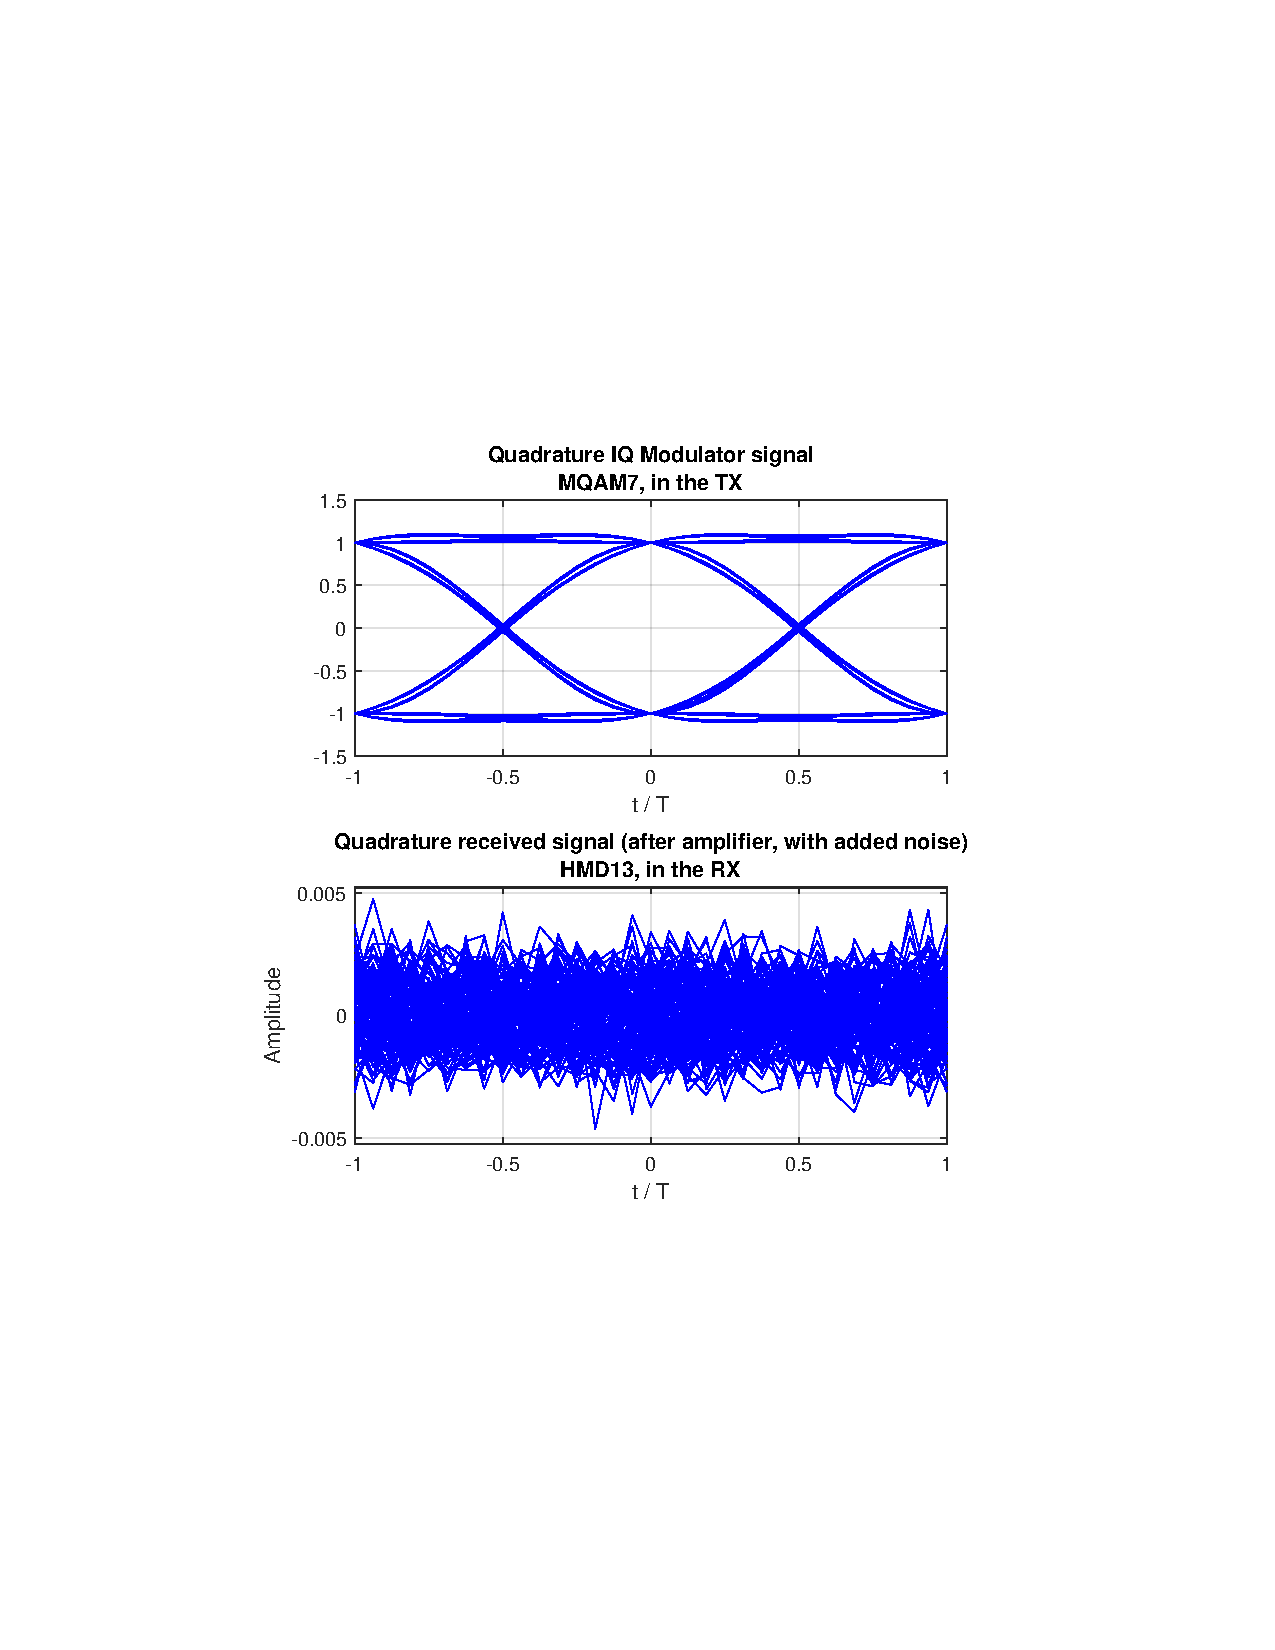
\includegraphics[clip, trim=4cm 7cm 4cm 7cm, 
		width=\textwidth]{./sdf/m_qam_system/figures/eyes/simulRc09Sp60Np60_q.pdf}
	\end{subfigure}
	
	\caption{
%		Eye diagrams without matched filtering with raised-cosine.
		Obtained
		at two different points in the system: optical output of transmitter on the top and
		the noisy signal at the bottom.
%		Simulation done with an optical power output of -60~dBm,
%		0~dBm at the local oscillator, a gain of $10^3$ at the amplifier, a noise
%		spectral density of $10^{-6}$ and a rolloff factor of
%		0.9.
		\label{fig:eyes_n_rc_60_09}}
	\end{minipage}]
\end{figure}

\begin{table}[H]
	\centering
	
	\begin{tabular}{|l|l|}
		\hline
		\multicolumn{2}{|c|}{ \textbf{Simulation Parameters} } \\
		\hline
		\textbf{Parameter}     & \textbf{Default Value}                                     \\\hline
				%		numberOfBitsGenerated  & $40000$	                                                \\\hline
		bitPeriod              & $1/32\times10^9$~s														\\\hline
		%		symbolRate		       &                                                     		\\\hline
		samplesPerSymbol       & $16$                                                       \\\hline
		%		symbolRate		       &                                                     		\\\hline
		%		pLength                & $5$                                                        \\\hline
		%		iqAmplitudesValues     & $\lbrace~\lbrace-1,~0\rbrace~,~\lbrace1,~0\rbrace~\rbrace$ \\\hline
		outputOpticalPower     & $-60$~dBm 													\\ \hline
		shaperFilter	       & RootRaisedCosine												\\ \hline
		outputFilter		   & RootRaisedCosine												\\ \hline
		rollOffFactor		   & 0.9														\\ \hline
		localOscillatorPower   & $0$~dBm                                                    \\ \hline
		localOscillatorPhase   & $0$                                                        \\ \hline
		%		transferMatrix         & $\lbrace~\lbrace \frac{1}{\sqrt{2}},~\frac{1}{\sqrt{2}},~\frac{1}{\sqrt{2}},~\frac{-1}{\sqrt{2}} \rbrace~\rbrace$ & \\ \hline
		responsivity           & $1$                                                        \\ \hline
		amplification          & $10^3$                                                     \\ \hline
		noisePower   & $10^{-6}$~V$^2$                             					\\ \hline
				theoreticalSNR  	   & $0~dB$                             					\\ \hline
		numericalSNR 		     & $0.0290907~dB$                             					\\ \hline
		numericalSNR Upper Bound (95\% confidence) & $0.120973~dB$                             					\\ \hline
		numericalSNR Lower Bound (95\% confidence) & $-0.064778~dB$                             					\\ \hline
		%		confidence             & $0.95$                                                     \\ \hline
		%		midReportSize          & $0$                                                        \\ \hline
	\end{tabular}
\end{table}
\begin{figure}[H]
		\centering
	\textbf{Root-Raised-Cosine Signal (roll-off=0.9) with Added  and Matched Filtering, SNR = 0~dB}
	\begin{minipage}{\linewidth}
		\centering
	\begin{subfigure}{.45\textwidth}
		\centering
		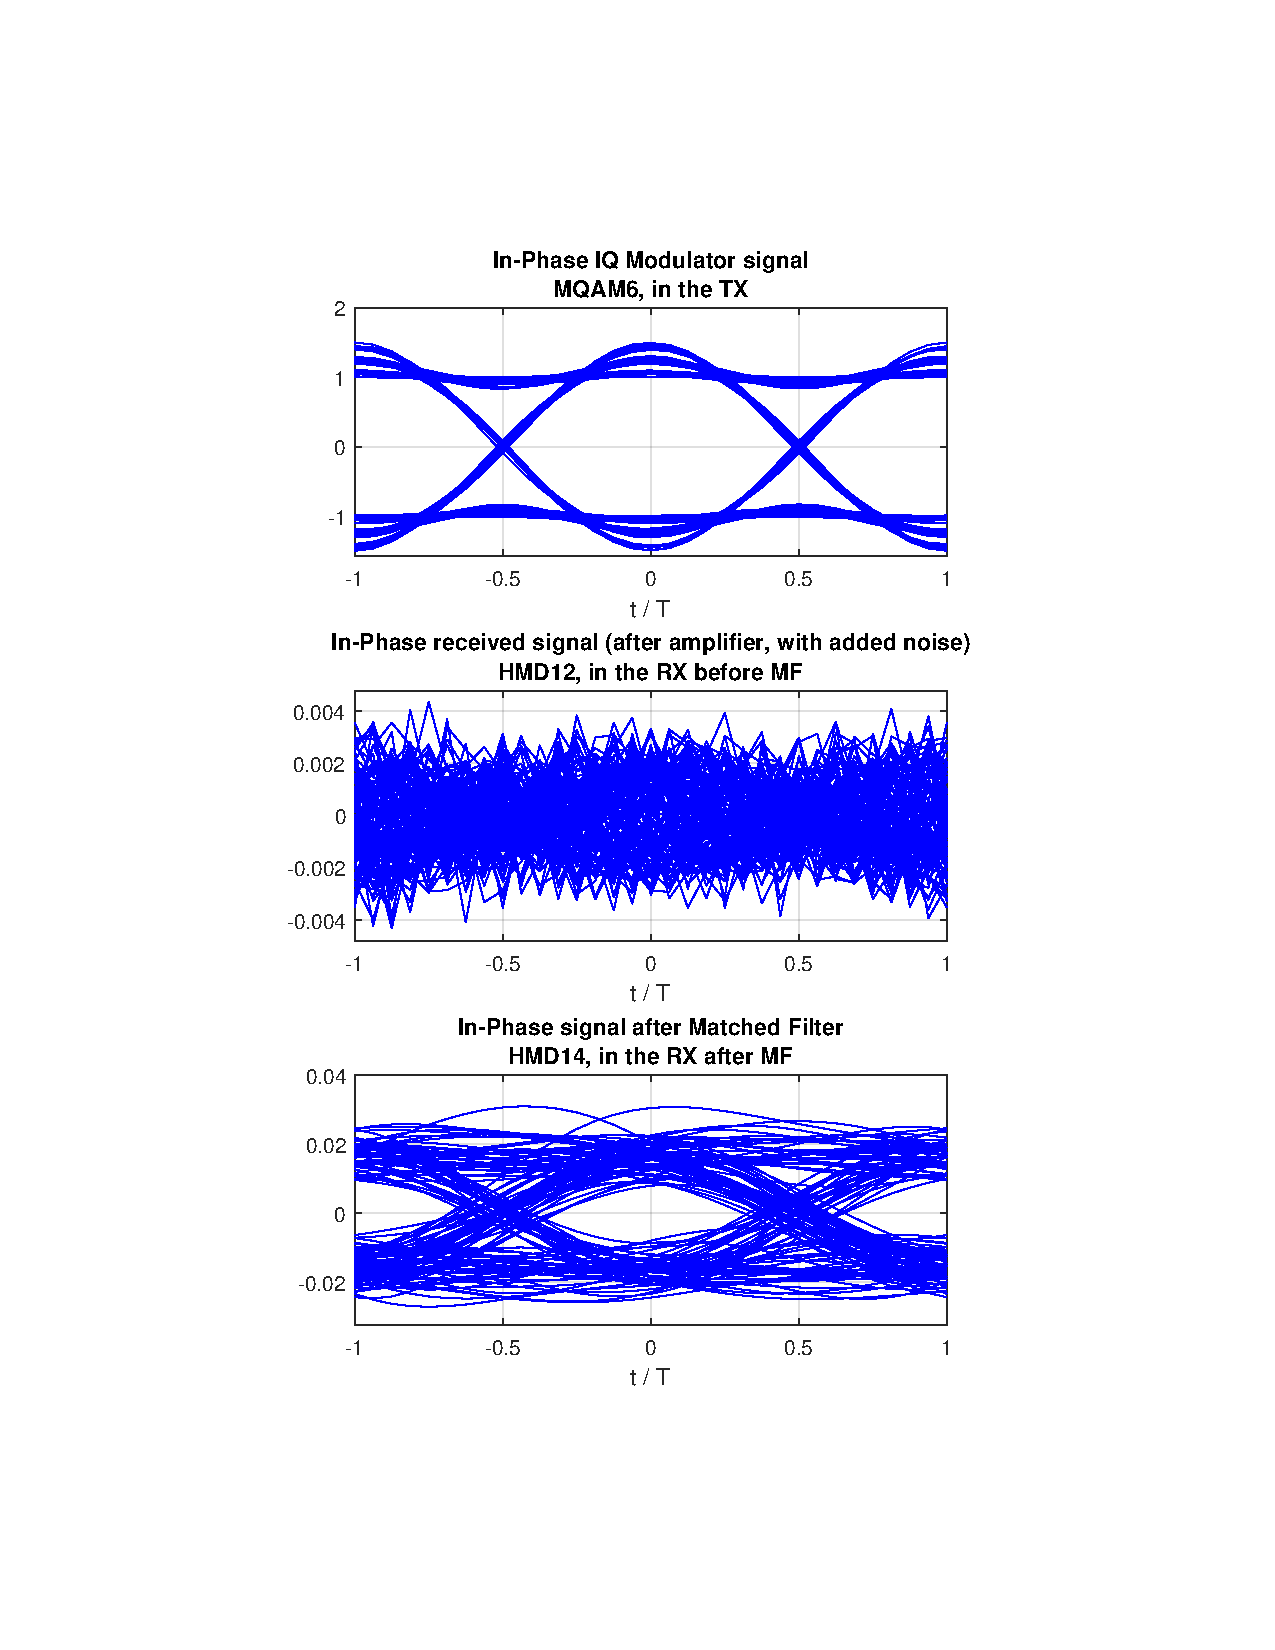
\includegraphics[clip, trim=4cm 4cm 4cm 4cm, 
		width=\textwidth]{./sdf/m_qam_system/figures/eyes/simulRrc09Sp60Np60_i.pdf}
	\end{subfigure}
	\begin{subfigure}{.45\textwidth}
		\centering
		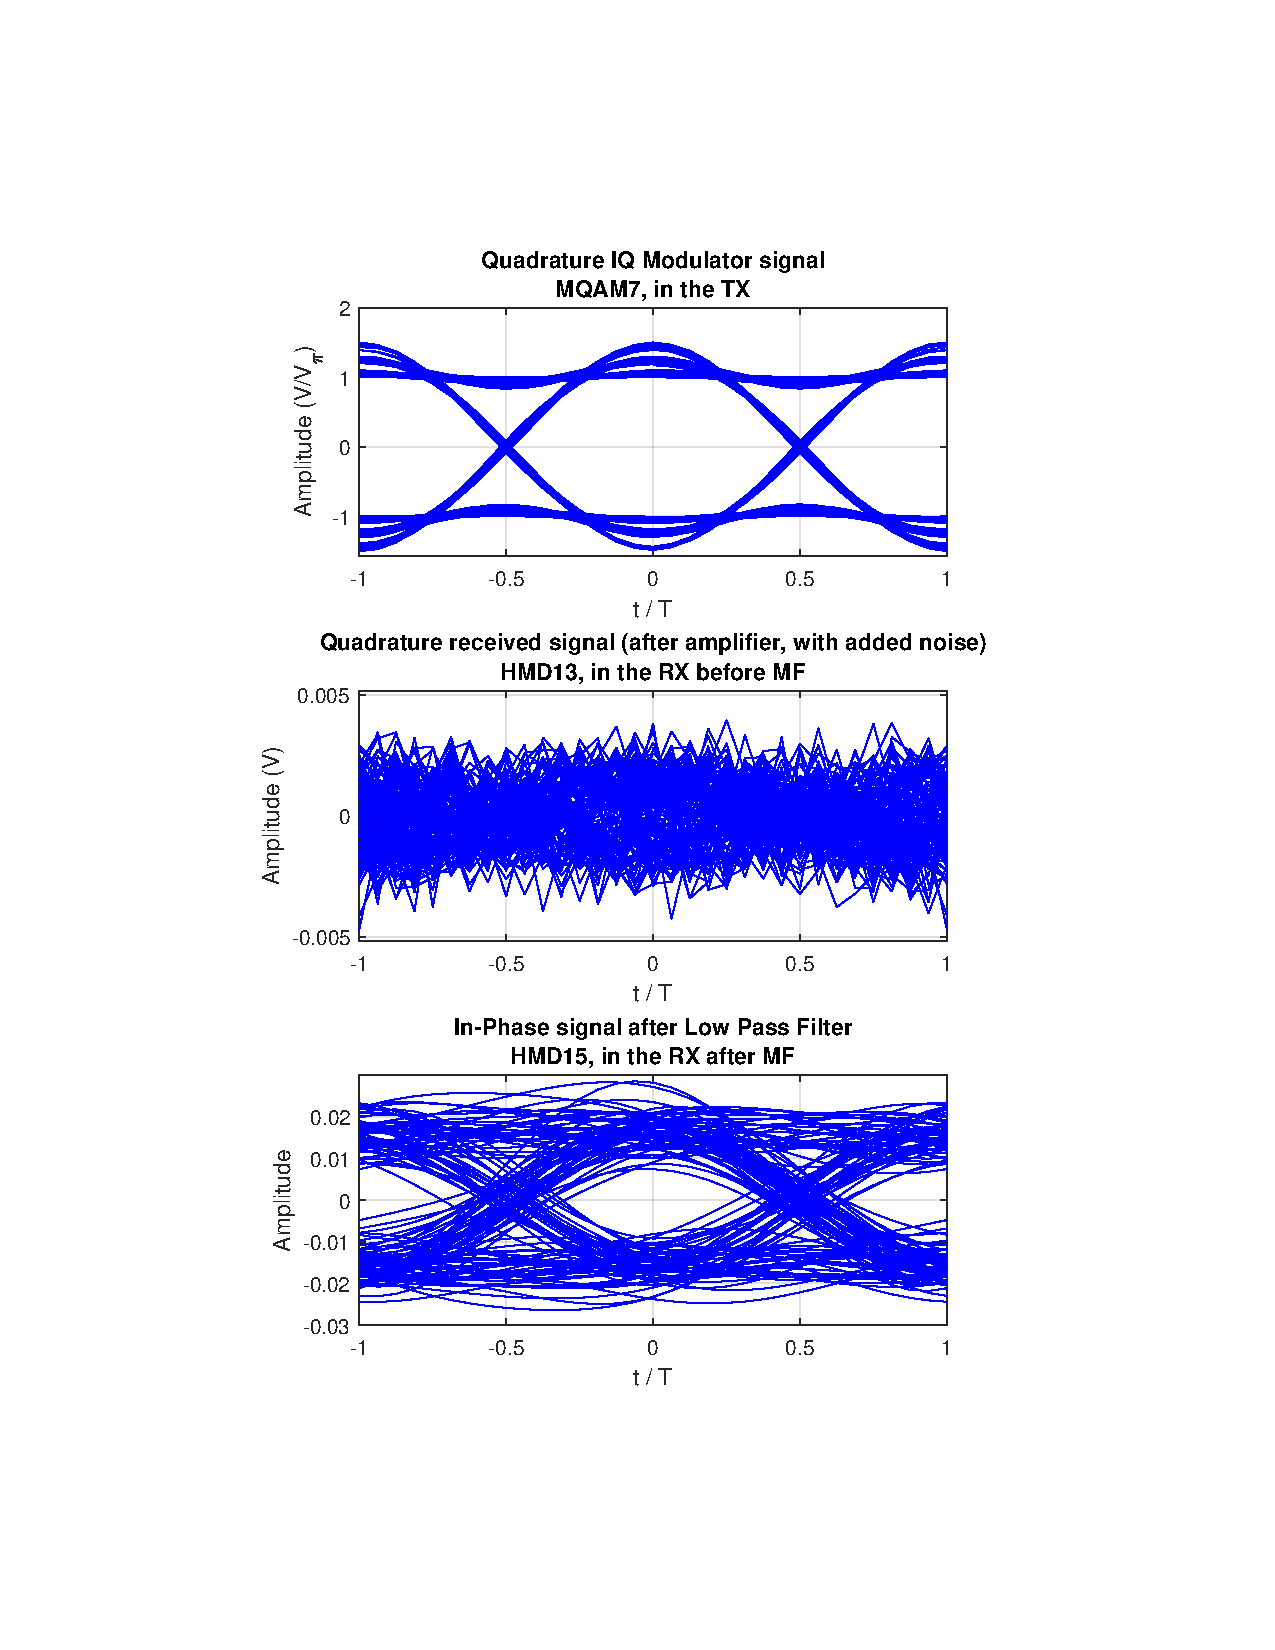
\includegraphics[clip, trim=4cm 4cm 4cm 4cm, 
		width=\textwidth]{./sdf/m_qam_system/figures/eyes/simulRrc09Sp60Np60_q.pdf}
	\end{subfigure}
	
	\caption{
%		Eye diagrams using matched filtering with root-raised-cosine.
		Obtained at three different points in the system: optical output of transmitter on the top;
		the amplified signal at the middle; and
		after the receiver filter.
%		Simulation done with an optical power output of -60~dBm, 0~dBm at the local oscillator, a gain of $10^3$ at the amplifier, a noise spectral density of $10^{-6}$ and a rolloff factor of 0.9.
		\label{fig:eyes_n_rrc_60_09}}
	\end{minipage}
\end{figure}


Figures~\ref{fig:eyes_n_rc_60_03} and~\ref{fig:eyes_n_rrc_60_09} show the same
case but using a roll-off factor of 0.3.
\begin{table}[H]
	\centering
	
	\begin{tabular}{|l|l|}
		\hline
		\multicolumn{2}{|c|}{ \textbf{Simulation Parameters} } \\
		\hline
		\textbf{Parameter}     & \textbf{Default Value}                                     \\\hline
		%		numberOfBitsGenerated  & $40000$	                                                \\\hline
		bitPeriod              & $1/32\times10^9$~s														\\\hline
		%		symbolRate		       &                                                     		\\\hline
		samplesPerSymbol       & $16$                                                       \\\hline
		%		symbolRate		       &                                                     		\\\hline
		%		pLength                & $5$                                                        \\\hline
		%		iqAmplitudesValues     & $\lbrace~\lbrace-1,~0\rbrace~,~\lbrace1,~0\rbrace~\rbrace$ \\\hline
		outputOpticalPower     & $-60$~dBm 													\\ \hline
		shaperFilter	       & RaisedCosine												\\ \hline
		outputFilter		   &   												\\ \hline
		rollOffFactor		   & 0.3														\\ \hline
		localOscillatorPower   & $0$~dBm                                                    \\ \hline
		localOscillatorPhase   & $0$                                                        \\ \hline
		%		transferMatrix         & $\lbrace~\lbrace \frac{1}{\sqrt{2}},~\frac{1}{\sqrt{2}},~\frac{1}{\sqrt{2}},~\frac{-1}{\sqrt{2}} \rbrace~\rbrace$ & \\ \hline
		responsivity           & $1$                                                        \\ \hline
		amplification          & $10^3$                                                     \\ \hline
		noisePower   & $10^{-6}$~V$^2$                             					\\ \hline
						theoreticalSNR  	   & $0~dB$                             					\\ \hline
		numericalSNR 		     & $-0.306456~dB$                             					\\ \hline
		numericalSNR Upper Bound (95\% confidence) & $-0.233164~dB$                             					\\ \hline
		numericalSNR Lower Bound (95\% confidence) & $-0.381006~dB$                             					\\ \hline
		%		confidence             & $0.95$                                                     \\ \hline
		%		midReportSize          & $0$                                                        \\ \hline
	\end{tabular}
\end{table}
\begin{figure}[H]
		\centering
	\textbf{Raised-Cosine Signal (roll-off=0.3) with Added Noise, SNR = 0~dB}
	\begin{minipage}{\linewidth}
		\centering
	\begin{subfigure}{.45\textwidth}
		\centering
		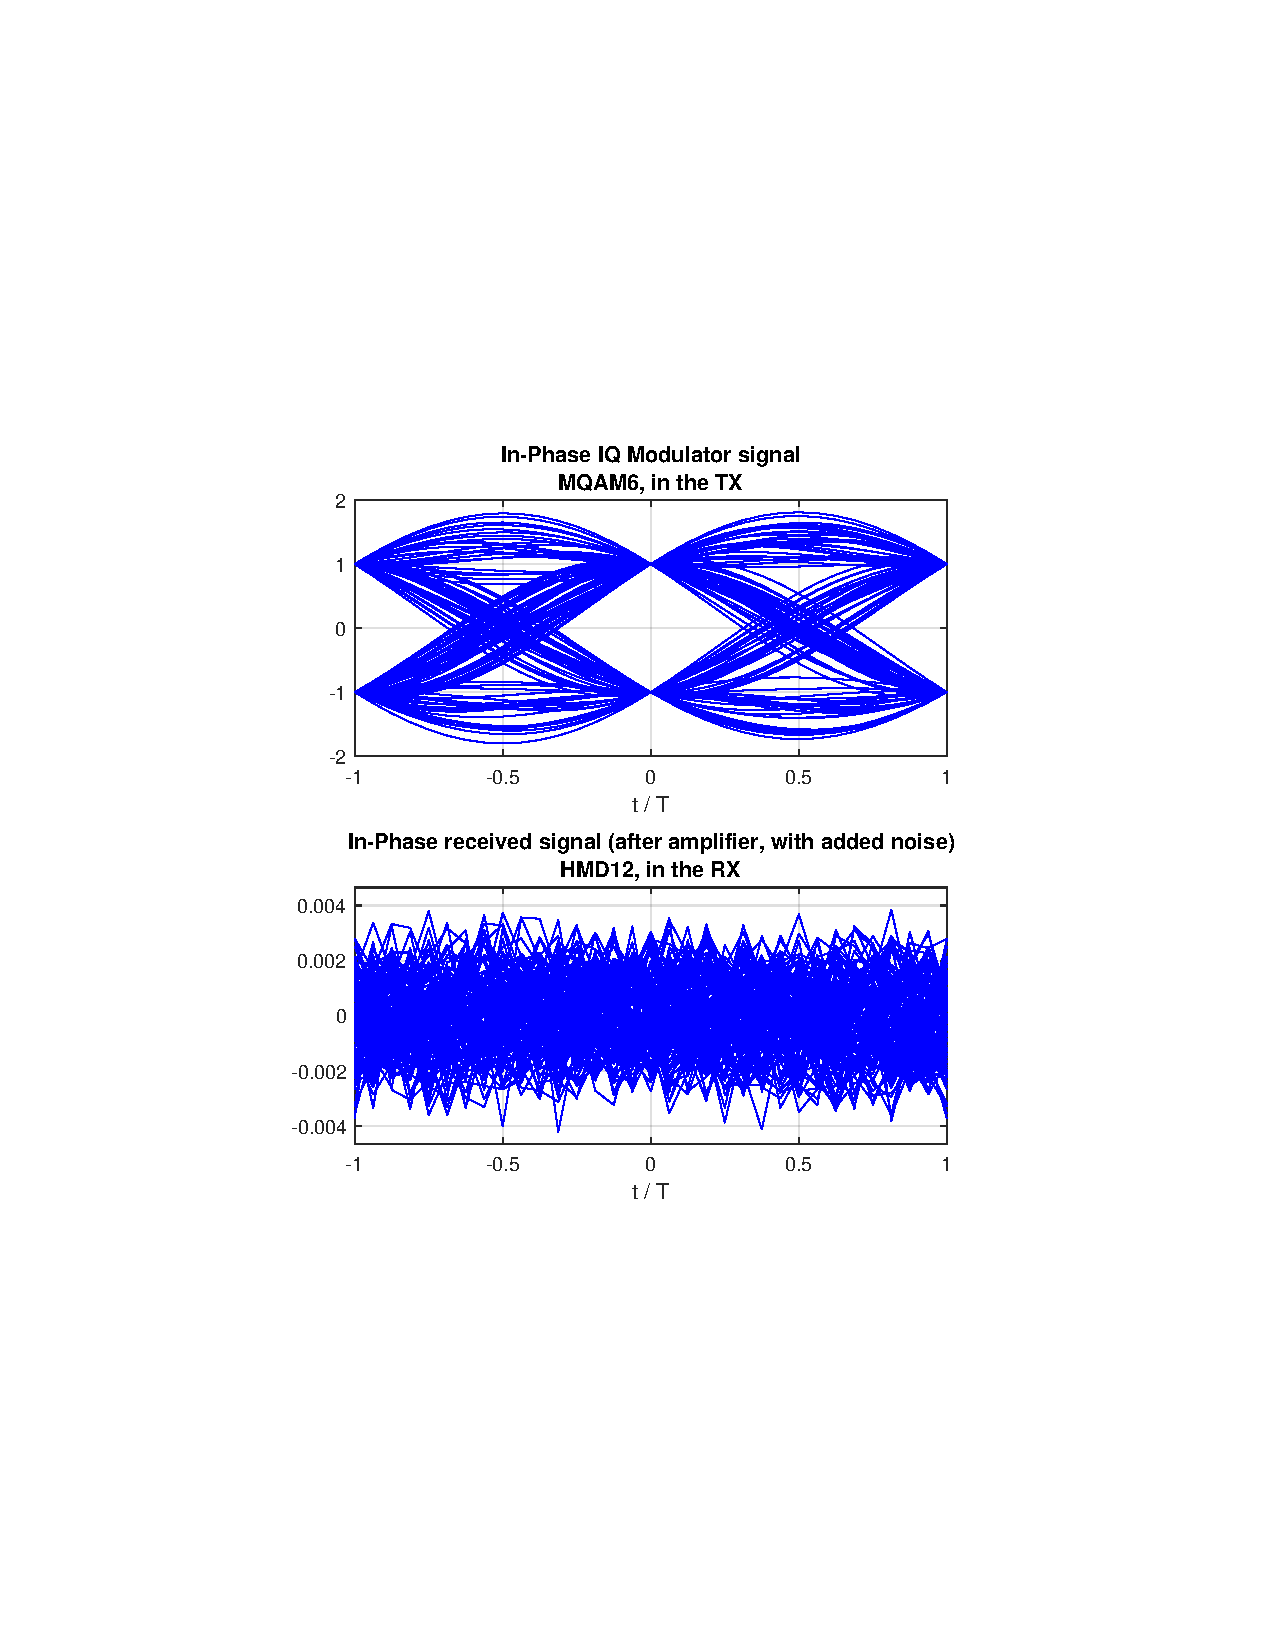
\includegraphics[clip, trim=4cm 7cm 4cm 7cm, 
		width=\textwidth]{./sdf/m_qam_system/figures/eyes/simulRc03Sp60Np60_i.pdf}
	\end{subfigure}
	\begin{subfigure}{.45\textwidth}
		\centering
		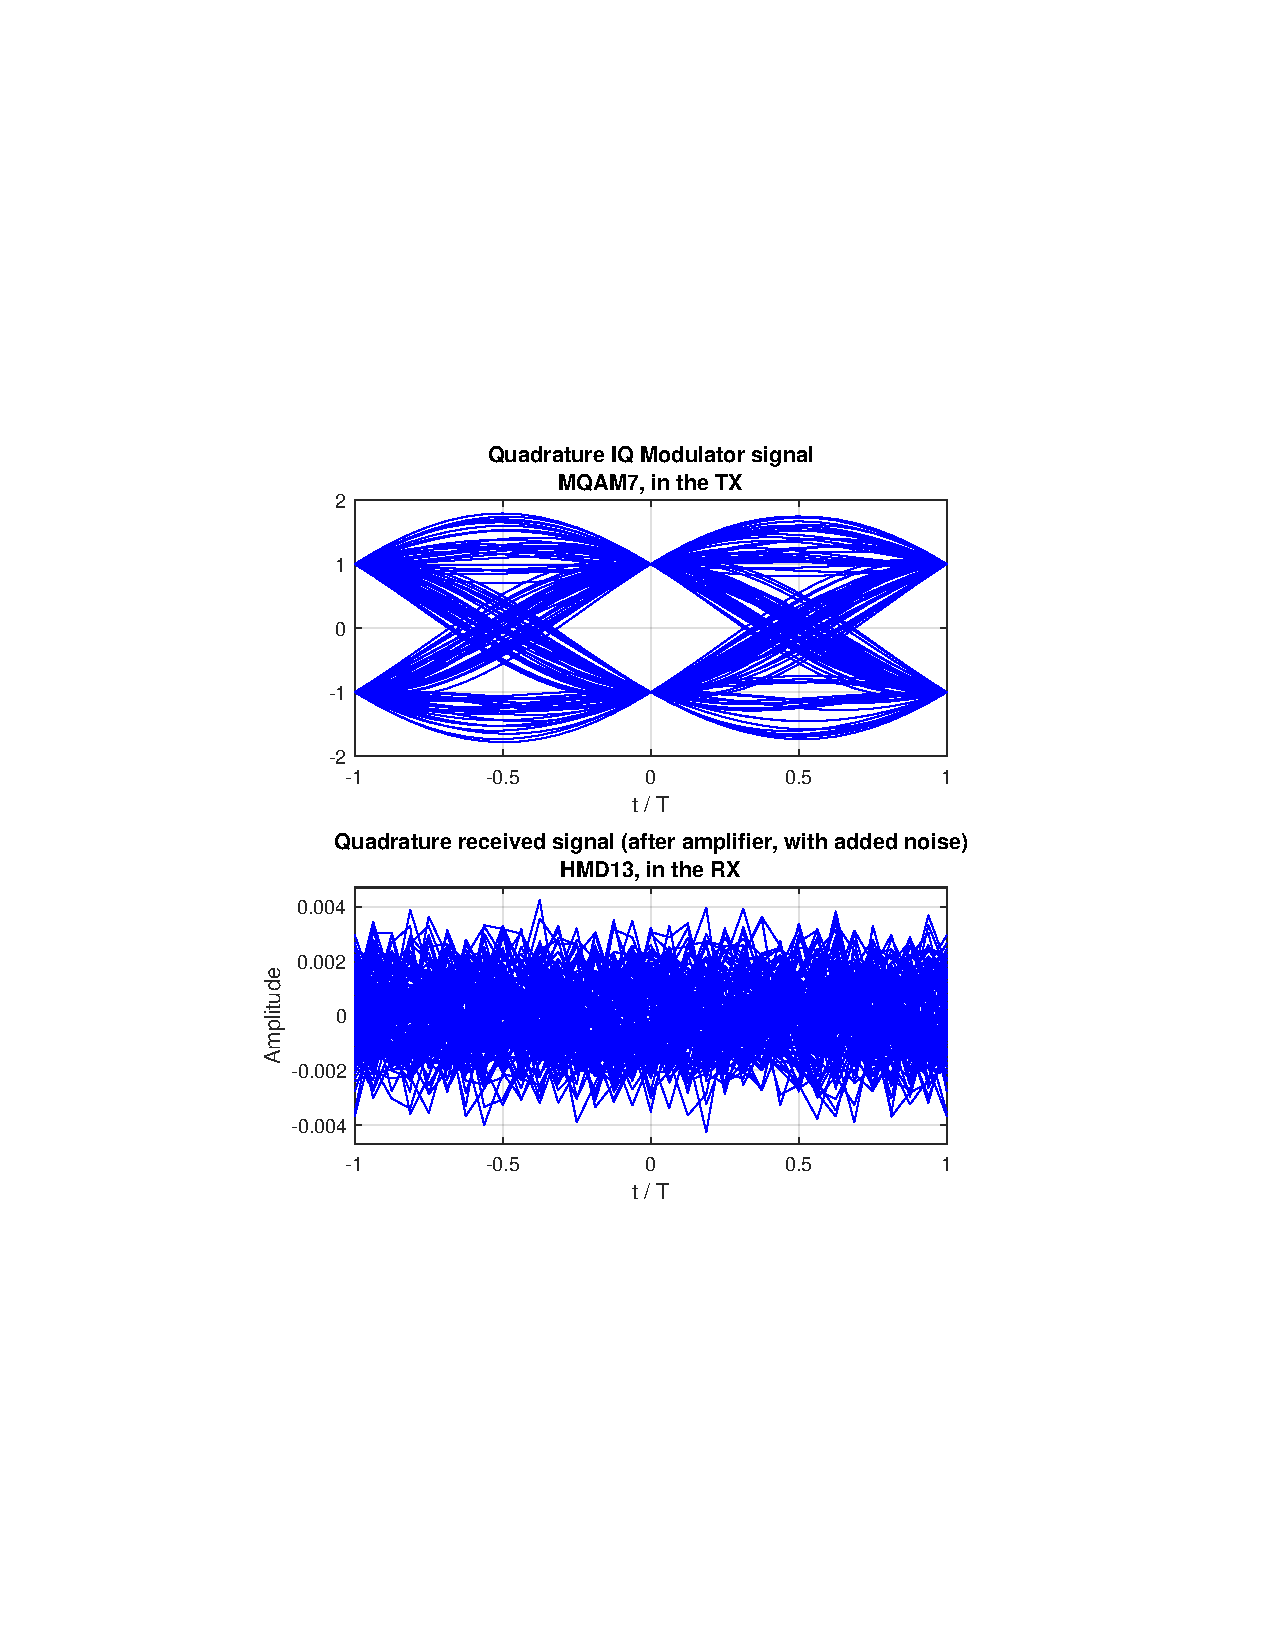
\includegraphics[clip, trim=4cm 7cm 4cm 7cm, 
		width=\textwidth]{./sdf/m_qam_system/figures/eyes/simulRc03Sp60Np60_q.pdf}
	\end{subfigure}
	
	\caption{
%		Eye diagrams without matched-filtering with raised-cosine.
		Obtained
		at two different points in the system: optical output of transmitter on the top and
		the noisy signal at the bottom.
%		Simulation done with an optical power output of -60~dBm, 0~dBm at
%		the local oscillator, a gain of $10^3$ at the amplifier, a noise spectral
%		density of $10^{-6}$ and a rolloff factor of 0.3.
		\label{fig:eyes_n_rrc_60_03}}
	\end{minipage}
\end{figure}
\begin{table}[H]
	\centering
	
	\begin{tabular}{|l|l|}
		\hline
		\multicolumn{2}{|c|}{ \textbf{Simulation Parameters} } \\
		\hline
		\textbf{Parameter}     & \textbf{Default Value}                                     \\\hline
		%		numberOfBitsGenerated  & $40000$	                                                \\\hline
		bitPeriod              & $1/32\times10^9$~s														\\\hline
		%		symbolRate		       &                                                     		\\\hline
		samplesPerSymbol       & $16$                                                       \\\hline
		%		symbolRate		       &                                                     		\\\hline
		%		pLength                & $5$                                                        \\\hline
		%		iqAmplitudesValues     & $\lbrace~\lbrace-1,~0\rbrace~,~\lbrace1,~0\rbrace~\rbrace$ \\\hline
		outputOpticalPower     & $-60$~dBm 													\\ \hline
		shaperFilter	       & RootRaisedCosine												\\ \hline
		outputFilter		   & RootRaisedCosine												\\ \hline
		rollOffFactor		   & 0.3														\\ \hline
		localOscillatorPower   & $0$~dBm                                                    \\ \hline
		localOscillatorPhase   & $0$                                                        \\ \hline
		%		transferMatrix         & $\lbrace~\lbrace \frac{1}{\sqrt{2}},~\frac{1}{\sqrt{2}},~\frac{1}{\sqrt{2}},~\frac{-1}{\sqrt{2}} \rbrace~\rbrace$ & \\ \hline
		responsivity           & $1$                                                        \\ \hline
		amplification          & $10^3$                                                     \\ \hline
		noisePower   & $10^{-6}$~V$^2$                             					\\ \hline
								theoreticalSNR  	   & $0~dB$                             					\\ \hline
		numericalSNR 		     & $0.0368278~dB$                             					\\ \hline
		numericalSNR Upper Bound (95\% confidence) & $0.09153~dB$                             					\\ \hline
		numericalSNR Lower Bound (95\% confidence) & $-0.0185722~dB$                             					\\ \hline
		%		confidence             & $0.95$                                                     \\ \hline
		%		midReportSize          & $0$                                                        \\ \hline
	\end{tabular}
\end{table}
\begin{figure}[H]
		\centering
	\textbf{Root-Raised-Cosine Signal (roll-off=0.3) with Added Noise and Matched Filtering,\\ SNR = 0~dB}
	\begin{minipage}{\linewidth}
		\centering
	\begin{subfigure}{.45\textwidth}
		\centering
		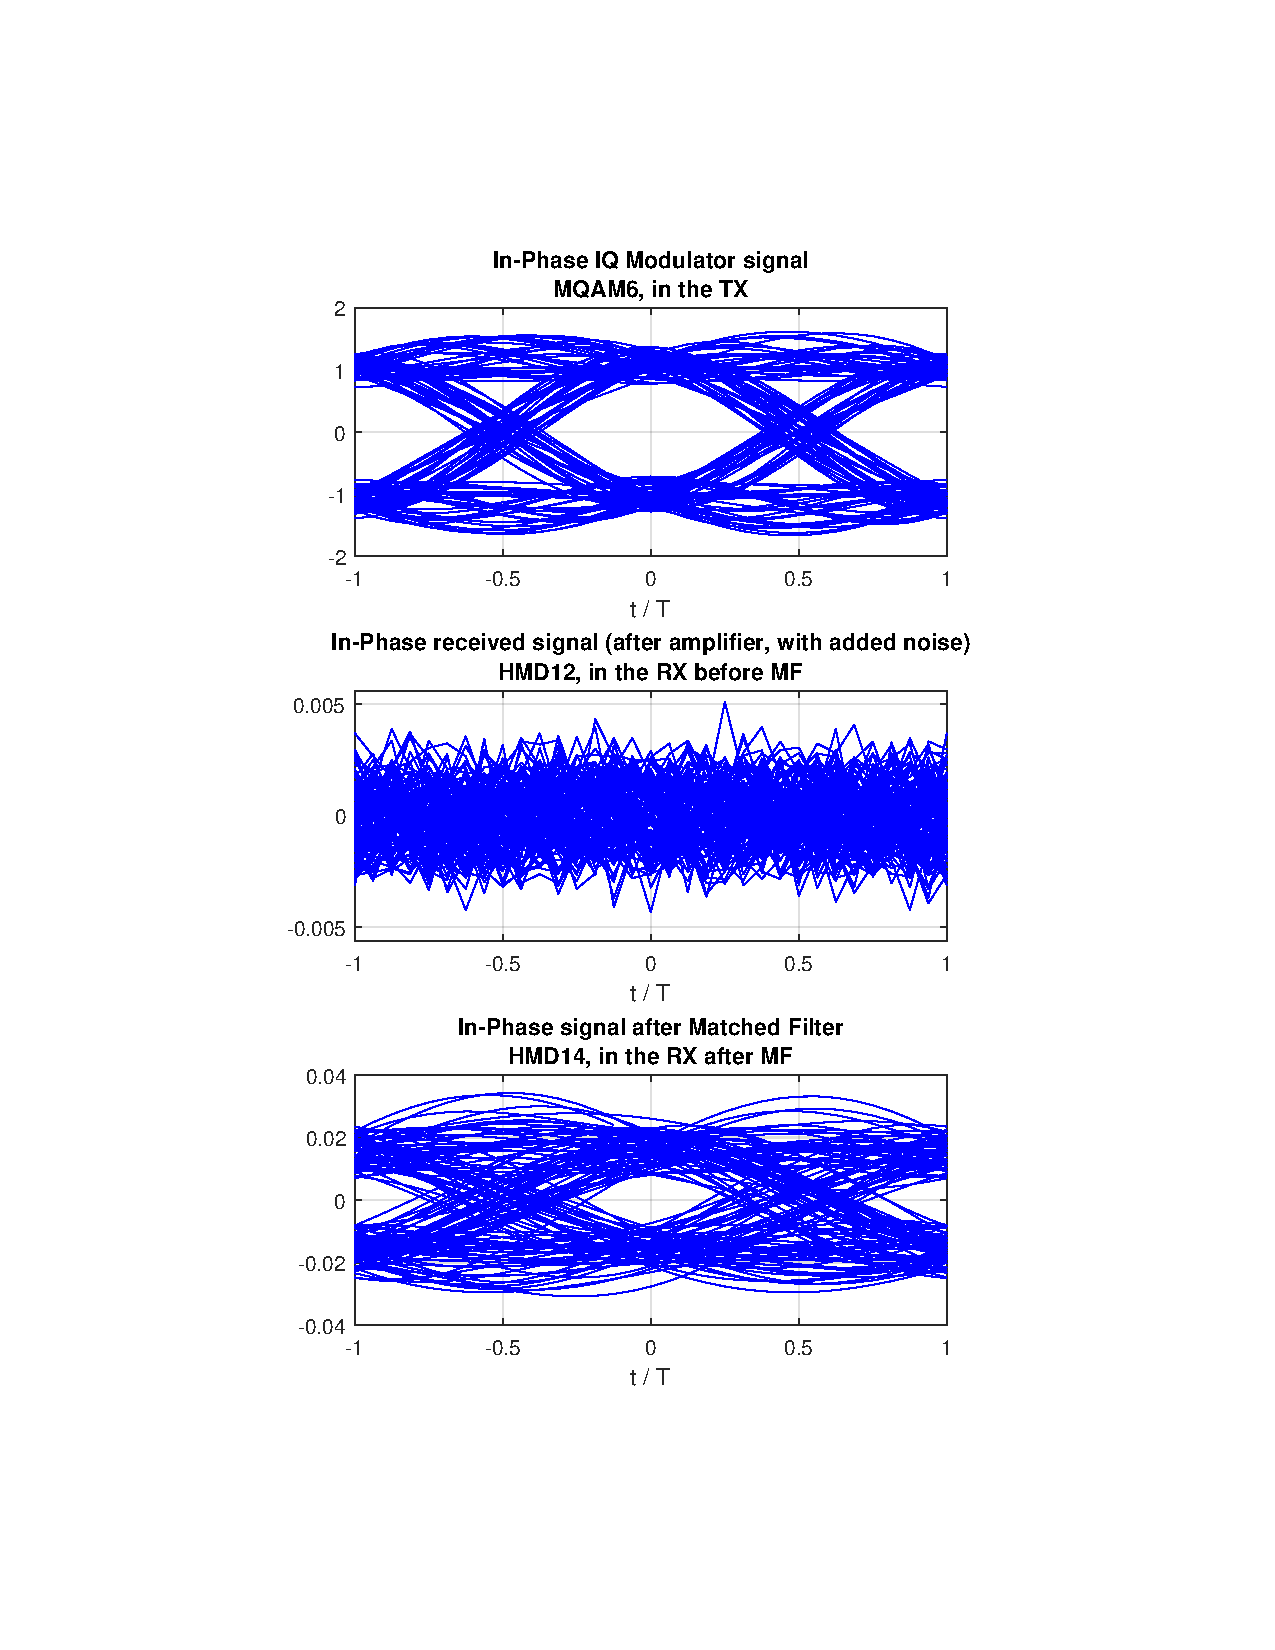
\includegraphics[clip, trim=4cm 4cm 4cm 4cm, 
		width=\textwidth]{./sdf/m_qam_system/figures/eyes/simulRrc03Sp60Np60_i.pdf}
	\end{subfigure}
	\begin{subfigure}{.45\textwidth}
		\centering
		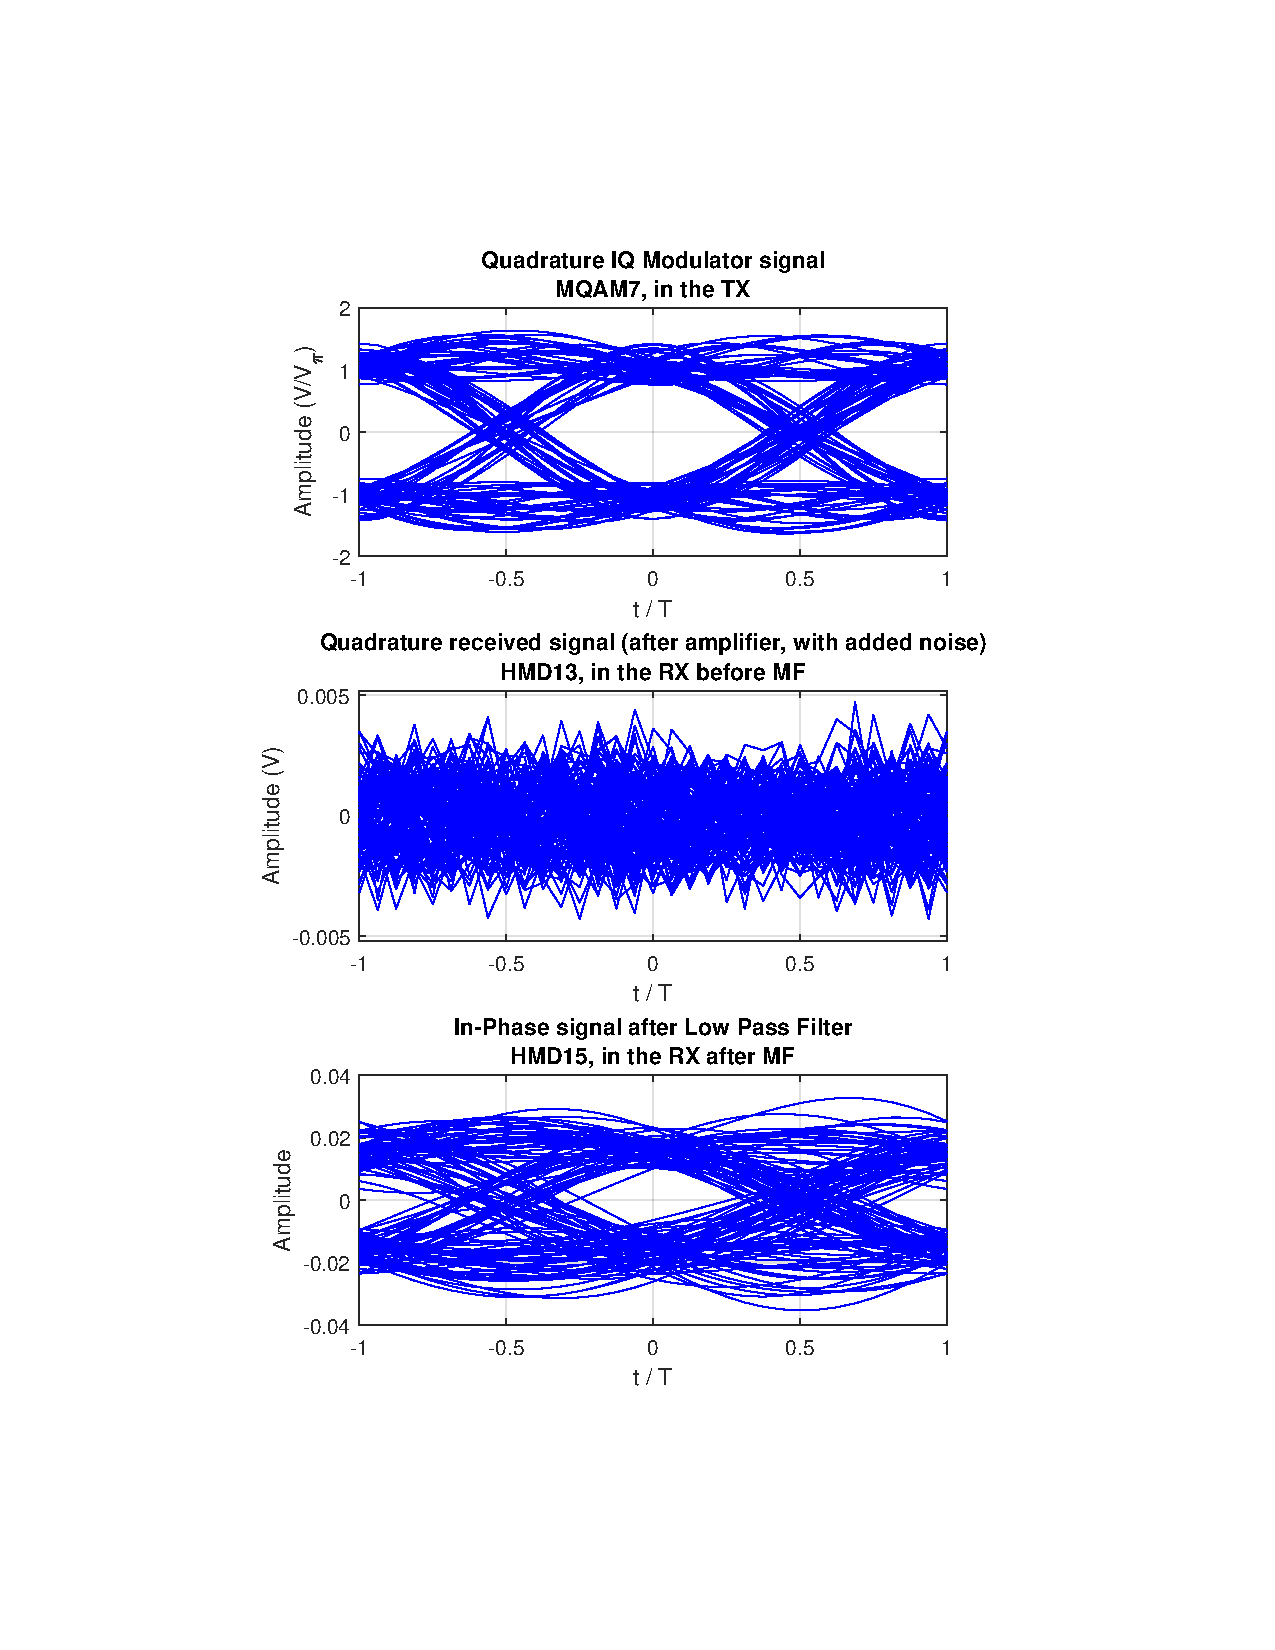
\includegraphics[clip, trim=4cm 4cm 4cm 4cm, 
		width=\textwidth]{./sdf/m_qam_system/figures/eyes/simulRrc03Sp60Np60_q.pdf}
	\end{subfigure}
	
	\caption{
%		Eye diagrams using matched filtering with root-raised-cosine.
		Obtained at three different points in the system: optical output of transmitter on the top;
		the amplified signal at the middle; and
		after the receiver filter.
%		Simulation done with an optical
%		power output of -60~dBm, 0~dBm at the local oscillator, a gain of $10^3$ at the
%		amplifier, a noise spectral density of $10^{-6}$ and a rolloff factor of
%		0.3.
		\label{fig:eyes_n_rc_60_03}}
	\end{minipage}
\end{figure}



\subsection*{BER Curves}

The simulated results show agreement with the theoretical curves, as can be seen in Figure~\ref{fig:ber_pseudorandom}.

\begin{table}[H]
	\centering
	\begin{tabular}{|l|l|}
	\hline
	\multicolumn{2}{|c|}{ \textbf{Simulation and Curve Parameters} } \\
		\hline
		\textbf{Parameter}     & \textbf{Default Value}                                     \\\hline
		numberOfBitsGenerated  & 
		$200000$	                                                \\\hline
		samplingRate           & 64 GHz															\\\hline
		symbolRate		       & 4, 16, 32, 64 
		GHz                                                    		\\\hline
		shaperFilter		   & With MF: RootRaisedCosine; Without MF: 
		RaisedCosine	    \\\hline
		receiverFilter		   & With MF: RootRaisedCosine; Without MF: no 
		filter 		\\\hline
		rollOff				   & 0.3														\\\hline
		%		samplesPerSymbol       & $16$                                                       \\\hline
		%		pLength                & $5$                                                        \\\hline
		%		iqAmplitudesValues     & $\lbrace~\lbrace-1,~0\rbrace~,~\lbrace1,~0\rbrace~\rbrace$ \\\hline
		outputOpticalPower     & Variable                                                   \\ \hline
		localOscillatorPower   & $0$~dBm                                                    \\ \hline
		%		localOscillatorPhase   & $0$                                                        \\ \hline
		%		transferMatrix         & $\lbrace~\lbrace	 \frac{1}{\sqrt{2}},~\frac{1}{\sqrt{2}},~\frac{1}{\sqrt{2}},~\frac{-1}{\sqrt{2}} \rbrace~\rbrace$ & \\ \hline
		responsivity           & $1$                                                        \\ \hline
		amplification          & $10^3$                                                     \\ \hline
		noisePower			   & $10^{-6}$~V$^2$                             					\\ \hline
		confidence             & $0.95$                                                     \\ \hline
		%			midReportSize          & $0$                                                        \\ \hline
	\end{tabular}
	\caption{Parameters for the theoretical curves and simulation results shown in Figure~\ref{fig:ber_pseudorandom}.\label{tab:ber_pseudorandom}}
\end{table}

\begin{figure}[H]
	\centering
		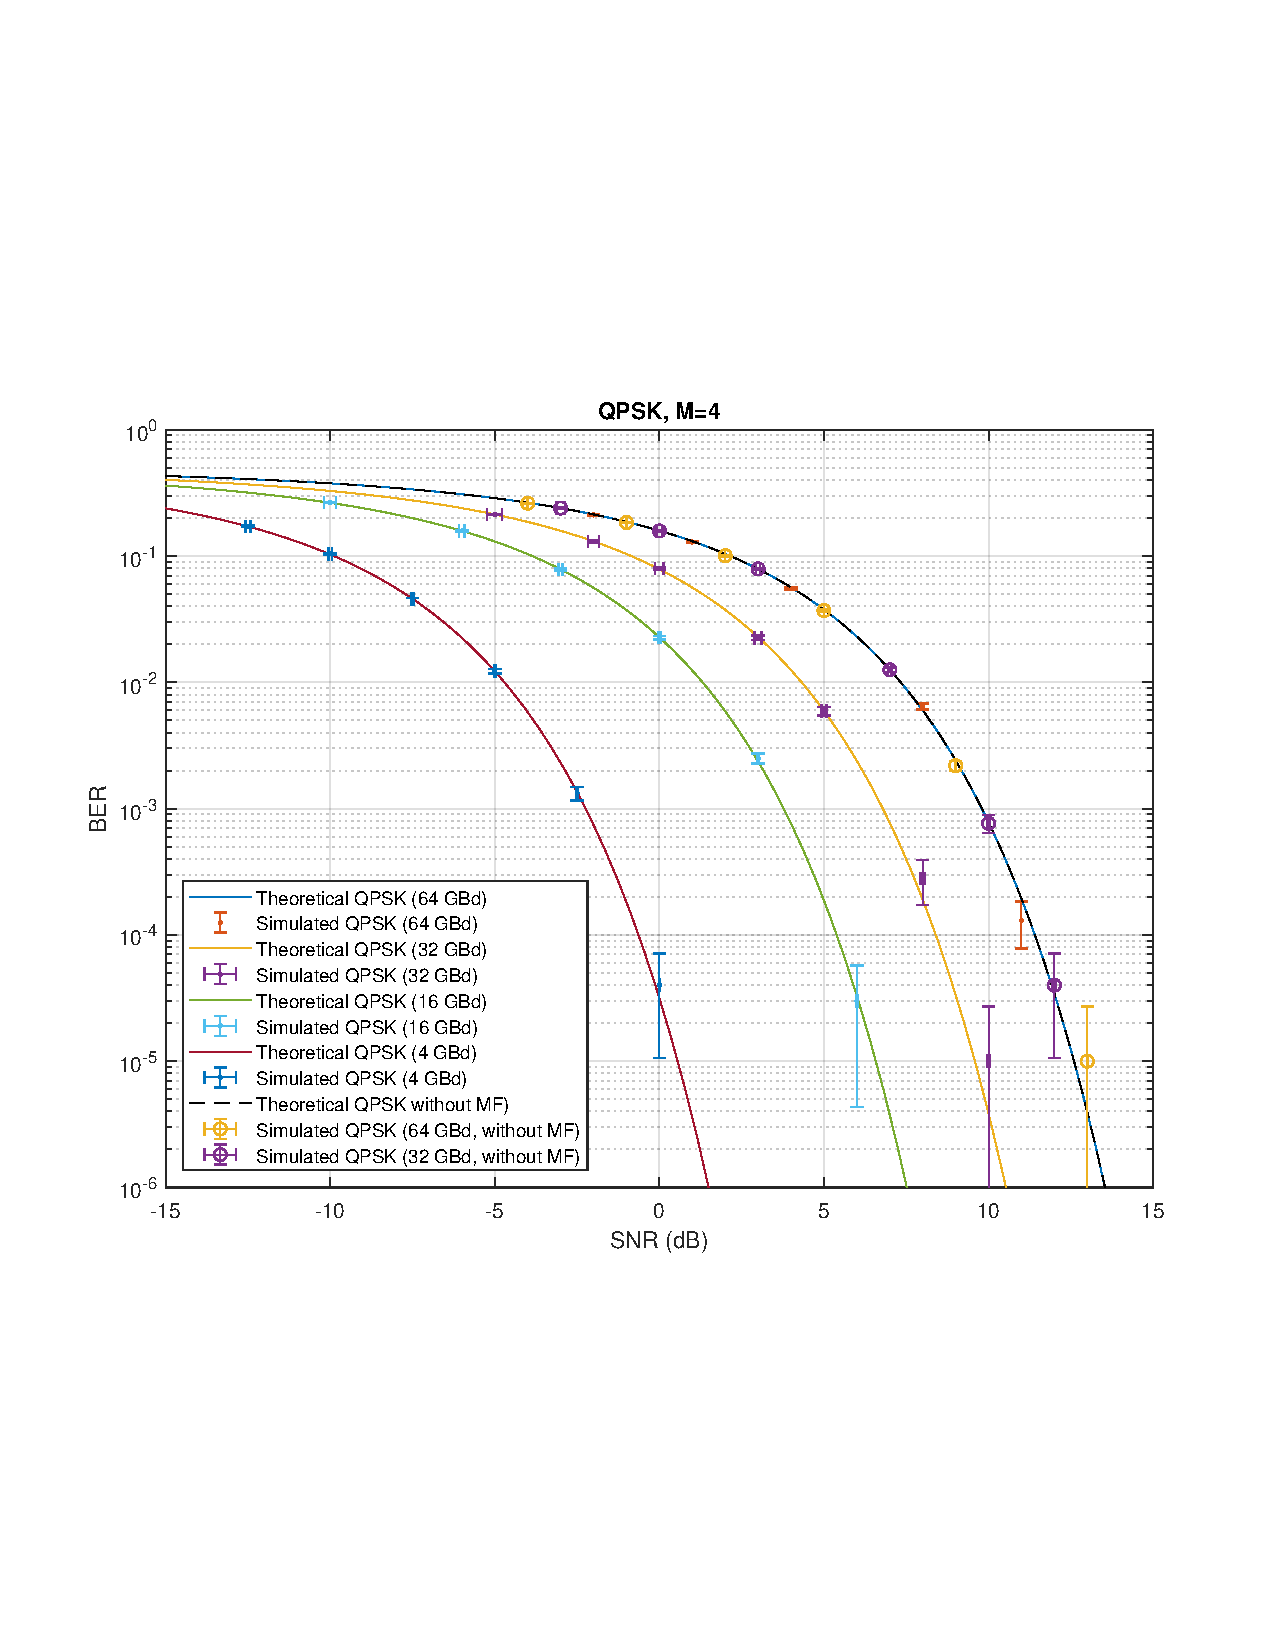
\includegraphics[clip, trim=0cm 6cm 0cm 6cm, 
		width=0.9\textwidth]{./sdf/m_qam_system/figures/teor_vs_simul.pdf}
	%			
\caption{QPSK theoretical BER values as a function of the output optical power in dBm.\label{fig:ber_pseudorandom}}
\end{figure}

%\subsection*{Comparative Analysis}

In this section we show the simulation results and compared them with the
theoretical predictions for an M-QAM system with $M=4$. Figure
\ref{fig:ber_pseudorandom} shows the variation of the BER with the optical power
of the signal, using $40000$ bits produced by a random number generator. The
noise power was set at $10^{-6}~V^2$, the local oscillator at $0~dBm$ and the
amplification at the transimpedance amplifier was set at $10^3$.
The red and blue lines represents the theoretical curve, with and without
matched filters, respectively. The the red and purple points represent the
simulated values for the same situation with the respective confidence margins.
The simulation agrees closely with the theoretical values.



%\begin{figure}[h]
%	\centering
%	\includegraphics[clip, trim=4cm 8cm 4cm 8cm, width=0.7\textwidth]{./sdf/m_qam_system/figures/BER_QPSK_sim_mf_20180205.pdf}
%	\caption{Simulation result using root-raised cosine matched filtering for a random binary sequence with $40000$ bits, a noise power of $10^{-6}$ and an amplification of $10^3$.}
%	\label{fig:ber_pseudorandom_mf}
%\end{figure}%


%\begin{figure}[H]
%	\centering
%	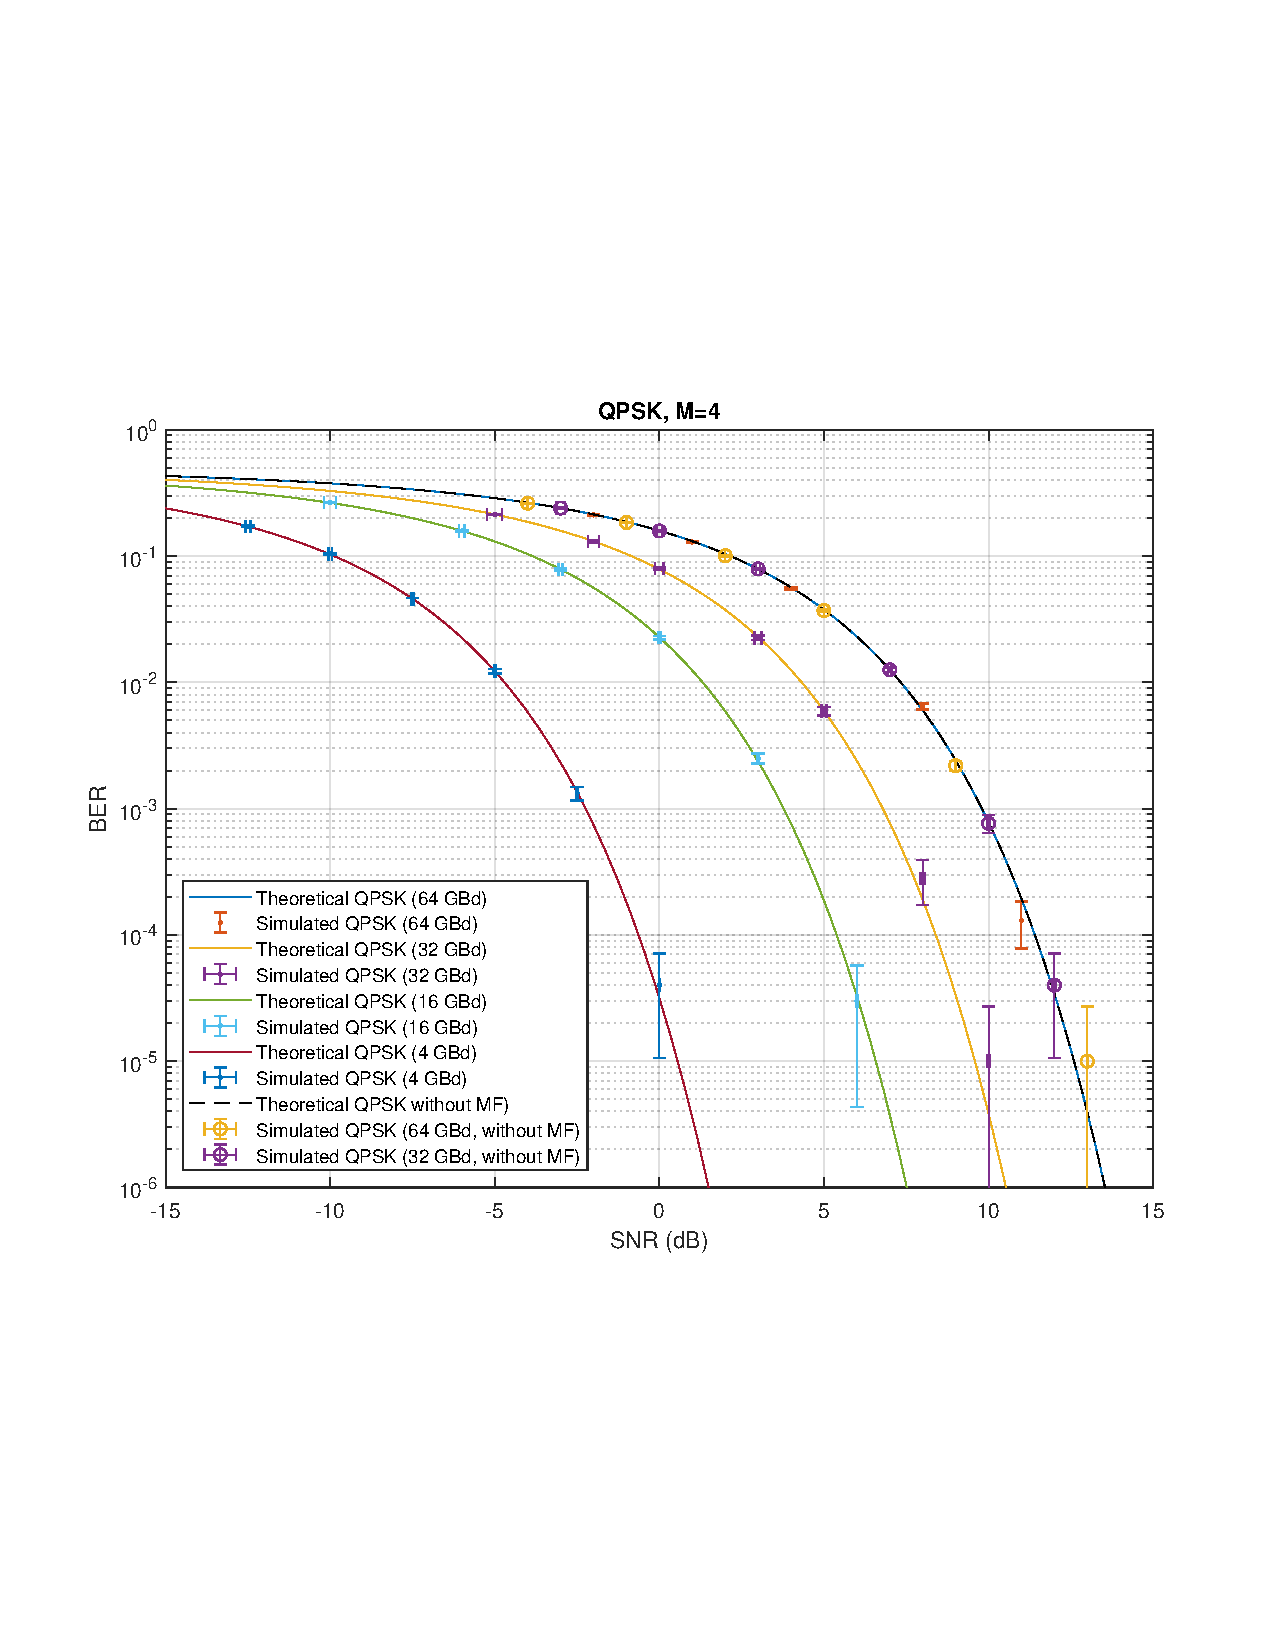
\includegraphics[clip, trim=4cm 8cm 4cm 8cm, width=0.7\textwidth]{./sdf/m_qam_system/figures/teor_vs_simul.pdf}
%	\caption{Simulation results for a random binary sequence with $40000$ bits, a noise power of $10^{-6}$ and an amplification of $10^3$. The simulated values which used a matched filter were obtained by shaping the pulse with a root-raised-cosine FIR filter and filtering the signal before the sample with the same filter. The results without matched filtering were obtained by using shaping the pulses with a raised-cosine filter. The margins shown were obtained for a 95\% confidence level.}
%\end{figure}%

\subsubsection*{Conclusions}
The use of a root-raised-cosine filters for shaping and filtering the signal
provides the best results, due to reducing noise while creating no inter-symbol
interference. The experimental BER curves agree with the theoretical values and
show the advantages of matched filtering.

\subsection{Experimental Analysis}
\begin{figure}[H]
	\centering
	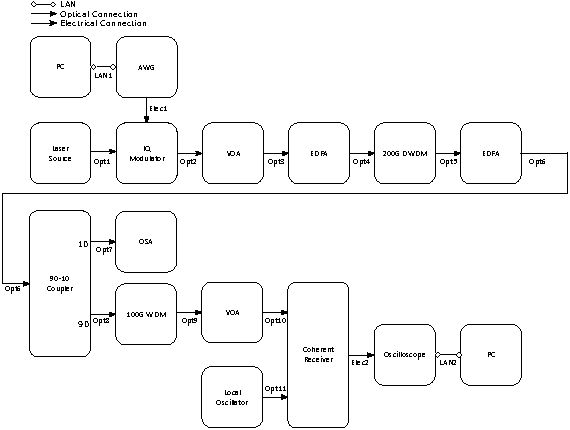
\includegraphics[width=\textwidth]{./sdf/m_qam_system/figures/mqamExperimental20180321.pdf}
	\caption{Experimental setup}
	\label{fig:experimental_mqam_setup}
\end{figure}

The setup shown in Figure~\ref{fig:experimental_mqam_setup} was used to obtain
experimental results to compare with the theory and validate the simulation. The
list of devices used for the setup is available in Table~\ref{tab:mqamdevices}. Tables~\ref{tab:rxParams} to~\ref{tab:edfaParams} show the devices' specifications.


%
%
\begin{table}[H]
	\centering
	\begin{tabulary}{1.0\textwidth}{|L|L|l|}
		\hline
		\textbf{Device}		& \textbf{Model}					& \textbf{Description}\\\hline
		Laser Source		& Yenista OSICS Band C/AG TLS Laser			& Optical laser source for modulate the signal \\\hline
		IQ Modulator 		& 22.5GHz IQ Modulator with automatic Bias Controller 	& \\\hline
		AWG 			& Keysight M8195A 					& \\\hline
		VOA			& 							& USB-Controlled Variable Optical Attenuator \\\hline
		EDFA			& Constelex Hydra-C-17-17 EDFA				& \\\hline
		200G DWDM		& 							& \\\hline
		EDFA			& Constelex Hydra-C-17-17 EDFA				& \\\hline
		90/10 Coupler		& 							& \\\hline
		OSA			& Apex Technologies AP-2043B 				& \\\hline
		100G WDM		& 							& \\\hline
		VOA			&							& \\\hline
		Local Oscillator	& Emcore CRTND3U02D ECL Laser				& \\\hline
		Coherent Receiver	& Picometrix CR-100D 					& \\\hline
		Oscilloscope		& Tektronix DP720004B				& \\\hline
	\end{tabulary}
	\caption{Devices in experimental setup.~\label{tab:mqamdevices}}
\end{table}

Tables~\ref{tab:rxParams} to~\ref{tab:edfaParams} list the relevant specifications for the devices used in the experimental setup.

\subsubsection{Device Specifications}
%
%\begin{table}[H]
%	\centering
%	\begin{tabulary}{1.0\textwidth}{|L|l|}
%		\hline
%		\multicolumn{2}{|c|}{\textbf{Tektronix DPO77002SX-R3 Oscilloscope, TekConnect channels}}	\\\hline
%			Analog channels bandwidth 	& 33~GHz 						\\\hline
%			Sample rate per channel		& 100~GS/s					\\\hline
%			Rise time (typical)			& 								\\
%			\multicolumn{1}{|r|}{10\% to 90\%} 				& 13~ps							\\
%			\multicolumn{1}{|r|}{20\% to 80\%}				&  9~ps							\\\hline
%			\multirow{2}{=}{Vertical noise, BWE on, max sample rate (typical)}
%										& 0.71\% of full scale 			\\
%										& 0.56\% of full scale @ 0~V offset (500~$\text{mV}_{FS}$) \\\hline
%			Timing resolution			& 10~ps							\\\hline
%			Sensitivity range			& $62.5~\text{mV}_{FS}$ to $6~\text{V}_{FS}$	\\\hline
%			Vertical resolution			& 8 bits (11 bits with averaging) \\\hline	
%			Effective number of bits	& 5.0 bits @ $500~\text{mV}_{FS}$, 100~GS/s \\\hline
%			Channel to channel Isolation (DC to 33~GHz) & 60~dB 	\\\hline
%	\end{tabulary}
%	\caption{\label{tab:rxParams}}
%\end{table}

\begin{table}[H]
	\centering
	\begin{tabulary}{1.0\textwidth}{|L|l|}
		\hline
		\multicolumn{2}{|c|}{\textbf{Tektronix DP720004B Oscilloscope, TekConnect channels}}	\\\hline
		Analog channels bandwidth 	& 20~GHz 						\\\hline
		Sample rate per channel		& 50~GS/s					\\\hline
		Rise time (typical)			& 								\\
		\multicolumn{1}{|r|}{10\% to 90\%} 				& 18~ps							\\
		\multicolumn{1}{|r|}{20\% to 80\%}				& 14~ps							\\\hline
		Vertical noise, bandwidth filter on, max sample rate 50 mV/div(typical) & 0.56\% of full scale @ 0~V offset (500~$\text{mV}_{FS}$) \\\hline
		Timing resolution			& 10~ps							\\\hline
		Sensitivity range 			& $200~\text{mV}_{FS}$ to $5~\text{V}_{FS}$	\\\hline
		Vertical resolution			& 8 bits (11 bits with averaging) \\\hline	
		Effective number of bits	& 5.5 bits @ $50~\text{mV}/{div}$, 100~GS/s \\\hline
	\end{tabulary}
	\caption{\label{tab:rxParamsNew}}
\end{table}

\begin{table}[H]
	\centering
	\begin{tabulary}{1.0\textwidth}{|L|l|}
		\hline
		\multicolumn{2}{|c|}{\textbf{Yenista OSICS TLS-AG Wide C-band}}	\\\hline
		Frequency Range (Wavelength Range) 	& 196.275 - 191.125 THz (1527.41 - 1568.57 nm) 	\\\hline
		Output Power		& 20 mW (+13~dBm)					\\\hline
		Power Range (typ.)	& +6 to +13.6~dBm			\\\hline
		Relative Frequency (Wavelength) Accuracy (typ.) & $\pm 0.5~\text{GHz}$ ($\pm~4~\text{pm}$)  \\\hline
		Absolute Frequency (Wavelength) Accuracy (typ.) & $\pm 1.5~\text{GHz}$ ($\pm~12~\text{pm}$)  \\\hline
		Frequency Setting Resolution & Down to 1 MHz \\\hline
		Instantaneous Linewidth (FWHM) & < 100 kHz \\\hline
		Power Stability & $\pm0.03~\text{dB}$ \\\hline
		Absolute Output Power Deviation Accross Tuning Range & $\pm0.2~\text{dB}$ \\\hline
		Side Mode Suppression Ratio & 60~dB	\\\hline
		Relative Intensity Noise & -145 dB/Hz \\\hline
	\end{tabulary}
	\caption{\label{tab:laserParams}}
\end{table}


\begin{table}[H]
	\centering
	\begin{tabulary}{1.0\textwidth}{|L|l|}
		\hline
		\multicolumn{2}{|c|}{\textbf{Local Oscillator Laser}}	\\\hline
		Optical Output Power Adjustment Range 	& +7 - +13.5 dBm 	\\\hline
		Optical Output Power Adjustment Range - high power variant		& 7 - 15.5~dBm					\\\hline
		Short term power variation	& 0.05~dB			\\\hline
		Optical Output Power Step Size & 0.01 dB \\\hline
		Operating Frequency (Wavelength) Range & 191.5 - 196.25~THz (1527.6 - 1565.5~nm)\\\hline
		Fine Tune Frequency Resolution	(typ.) & 1 MHz \\\hline
		Fine Tune Frequency Range 		& -6 -~+6GHz \\\hline
		Frequency Accuracy EOL			& $\pm 2.5~\text{GHz}$ \\\hline
		Frequency Accuracy EOL (25 GHz spacing variant)			& $\pm 1.5~\text{GHz}$ \\\hline
		Instantaneous Linewidth (FWHM)		& 100~kHz \\\hline
		Relative Intensity Noise (+13dBm output) & -145 dB/Hz \\\hline
		Relative Intensity Noise (+7dBm output) & -140 dB/Hz \\\hline
		Side Mode Suppression Ratio (typ.)& 55 dB \\\hline
		Back reflection					& -14 dB \\\hline
		Optical Isolation 				& 30 dB \\\hline
		SSER	(typ.)						& 55 dB \\\hline
		Polarization Extinction Ratio & 20 dB \\\hline
	\end{tabulary}
	\caption{\label{tab:loParams}}
\end{table}

\begin{table}[H]
	\centering
	\begin{tabulary}{1.0\textwidth}{|L|l|}
		\hline
		\multicolumn{2}{|c|}{\textbf{Balanced Receiver}}	\\\hline
		Wavelength Range	& 1525 - 1570 nm \\\hline
		Bit Rate (max)		& 32 Gb/s		\\\hline
		Signal Input Power	& -6 dBm \\\hline
		Polarization Extinction Ratio & 18 dB \\\hline
		LO input Power 		& 16 dBm \\\hline
		I/Q relative phase in Mixer & \\
		\multicolumn{1}{|r|}{minimum} & 85~deg							\\
		\multicolumn{1}{|r|}{typical} & 90 deg			\\
		\multicolumn{1}{|r|}{maximum}&  95 deg			\\\hline
		I/Q phase stability in mixer (over lifetime) & -2 - +2 deg \\\hline
		PBS mixer excess loss	& 3.1 dB \\\hline
		Optical input return loss & -27 dB \\\hline
		Bandwidth (-3 dB elec.)	& 18.5 - 28~GHz \\\hline
		Low frequency cutoff	& 100 kHz \\\hline
		Group delay variation  & \\
		\multicolumn{1}{|r|}{0.1 - 15 GHz} & -3 - +3 ps\\
		\multicolumn{1}{|r|}{15 - 25 GHz} & -9 - +9 ps	\\\hline
		CMMR (signal input)			&\\
		\multicolumn{1}{|r|}{DC} 	& -17 dB\\
		\multicolumn{1}{|r|}{22GHz} & -16 dB\\\hline
		CMMR (LO input)			&\\
		\multicolumn{1}{|r|}{DC} 	& -12 dB\\
		\multicolumn{1}{|r|}{22GHz} & -10 dB\\\hline
		Linearity					& 5\% \\\hline
		Temporal Skew 				& \\
		\multicolumn{1}{|r|}{P/N outputs} 	& 3 ps\\
		\multicolumn{1}{|r|}{Across all four channels} & 10 ps\\\hline
		Photodiode dark current ($25^o$C)	& 100 nA \\\hline
		Photodiode responsivity @1550 nm & 0.64 A/W \\\hline
		Effective responsivity (both inputs) & 0.05 A/W \\\hline
	\end{tabulary}
	\caption{\label{tab:pinParams}}
\end{table}

\begin{table}[H]
	\centering
	\begin{tabulary}{1.0\textwidth}{|L|l|}
		\hline
		\multicolumn{2}{|c|}{\textbf{Constelex Hydra-C EDFA}}	\\\hline
		Input wavelength range 	& 1530-1565 nm 	\\\hline
		Saturated output power 	& 13 -21 dBm   	\\\hline
		Input power 			& -20 - +3 dBm 	\\\hline
		Small signal gain (Pin = -20dBm)	& >28 dB		\\\hline
		Noise Figure (Pin = -10dBm @1555 nm)		& <4 dB \\\hline
	\end{tabulary}
	\caption{\label{tab:edfaParams}}
\end{table}

\begin{table}[H]
	\centering
	\begin{tabulary}{1.0\textwidth}{|L|l|}
		\hline
		\multicolumn{2}{|c|}{\textbf{Keysight M8195A AWG}}	\\\hline
		Sample Rate 	& 65 GSa/s 	\\\hline
		Analog Bandiwidth (typ.)	& 25 GHz   	\\\hline
		Vertical Resolution 			& 8 bits 	\\\hline
		Amplitude (single ended)	& 75 $\text{mV}_{PP}$ to 1 $\text{V}_{PP}$		\\\hline
		Amplitude Resolution		& 200 $\mu\text{V}$ \\\hline
		Intrinsic Random Jitter		& < 200 fs \\\hline
		Rise time (typical)			& 								\\
		\multicolumn{1}{|r|}{20\% to 80\%}				&  18~ps							\\\hline
	\end{tabulary}
	\caption{\label{tab:awgParams}}
\end{table}

\begin{table}[H]
	\centering
	\begin{tabulary}{1.0\textwidth}{|L|l|}
		\hline
		\multicolumn{2}{|c|}{\textbf{22.5 GHz IQ Modulator with automatic Bias Controller}}	\\\hline
		Wavelength Range					& 1520 - 1580 nm \\\hline
		Electro Optical Bandwidth (min.)	& 22 GHz 	\\\hline
		Electro Optical Bandwidth (typ.) 	& 25~GHz\\\hline
		Optical Return Loss 				& 30 dB 	\\\hline
		Electrical Input High Frequency	3 dB point (typ.)	& 40 GHz	\\\hline
		Electrical Input High Frequency	3 dB point (max.)	& 65 kHz	\\\hline
		Electrical input Gain Ripple (typ.) & $ \pm 1~\text{dB}$ \\\hline
		Gain delay ripple (max.)			& $\pm50~\text{ps}$ \\\hline
	\end{tabulary}
	\caption{\label{tab:iqModParams}}
\end{table}



\subsection{Intradyne detection}
Figures~\ref{fig:expBer} to~\ref{fig:expBerOutSnr} show the BER curves obtained resorting to the OptDSP libraries for signal processing. The
post-processing is done offline and several processing stages, including signal synchronization, frequency offset correction,
phase offset correction and adaptive equalization. The SNR used to plot the experimental data points in Figure~\ref{fig:expBer} is estimated offline, based on spectral analysis of the waveforms obtained in the oscilloscope. The SNR in Figure~\ref{fig:expBerOutSnr} is also calculated offline, but through a different method more appropriate to the estimation of SNR from constellation points, commonly known as $M_2M_4$, or the moments method~\cite{matzner93}.

The  experimental results found here were obtained for two different symbol rates, 4 GBd and 16 GBd.

%\begin{figure}[H]
%	\centering
%	\includegraphics[clip, trim=4cm 8cm 4cm 8cm, width=0.7\textwidth]{./sdf/m_qam_system/figures/experimentalTxSnr4Sr16.pdf}
%	\caption{Part of the signal sent to the IQ modulator. Symbol rate of 16 GHz, with a sampling rate of 64 GHz.}
%	\label{fig:newQamTxSig}
%\end{figure}
%
%\begin{figure}[H]
%	\centering
%	\includegraphics[clip, trim=4cm 8cm 4cm 8cm, width=0.7\textwidth]{./sdf/m_qam_system/figures/experimentalRxSnr4Sr16.pdf}
%	\caption{Part of the signal received at the oscilloscope. Not synchronized with the signal of figure~\ref{fig:newQamTxSig}. Symbol rate of 16 GHz, sampling rate of 100 GHz, estimated SNR of 4.4 dB.}
%	\label{fig:newQamRxSig}
%\end{figure}


%\begin{figure}[H]
%	\centering
%	\includegraphics[clip, trim=4cm 8cm 4cm 8cm, width=0.7\textwidth]{./sdf/m_qam_system/figures/experimentalConstSnr4Sr16.pdf}
%	\caption{Constellation obtained at the end of the DSP process for a signal with 16 GHz symbol rate, with a 100 GHz sampling rate at the receiver and estimated SNR of 4.4 dB prior to the DSP.}
%	\label{fig:newExpConst}
%\end{figure}

%\begin{figure}[H]
%	\centering
%	\includegraphics[clip, trim=4cm 8cm 4cm 8cm, width=0.7\textwidth]{./sdf/m_qam_system/figures/experimentalVsTeor3.pdf}
%	\caption{Comparison of theoretical BER curves against obtained results. SNR values are estimated from the waveforms obtained at the oscilloscope.}
%	\label{fig:expBer}
%\end{figure}

\begin{figure}[H]
	\centering
	\begin{minipage}{0.43\textwidth}
	\centering
%	\textbf{4~GBd}
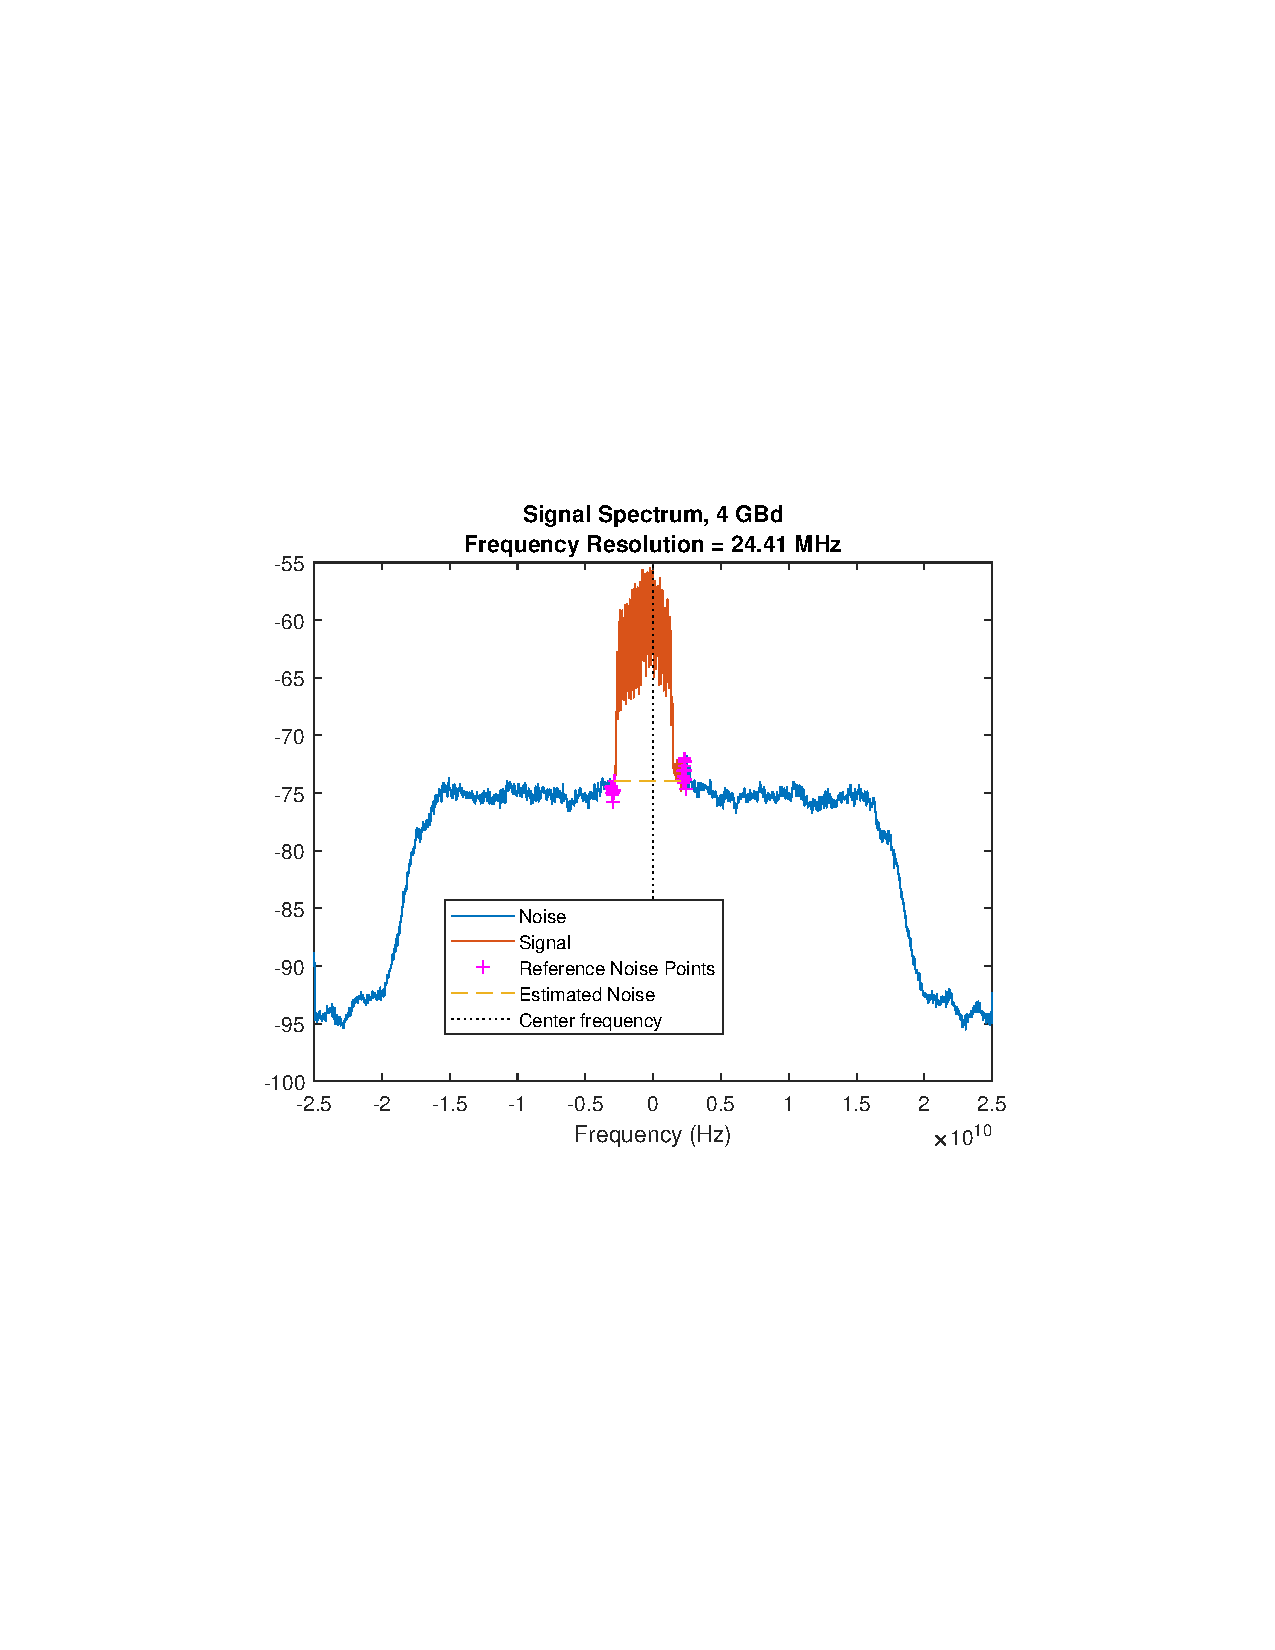
\includegraphics[clip, trim=4cm 8cm 4cm 8cm, width=1\textwidth]{./sdf/m_qam_system/figures/expResults/4GBdSpectrum.pdf}

\subcaption{\label{fig:4GBdSpectrum}}
	\end{minipage}
\begin{minipage}{0.43\textwidth}
		\centering
%	 \textbf{16~GBd}
	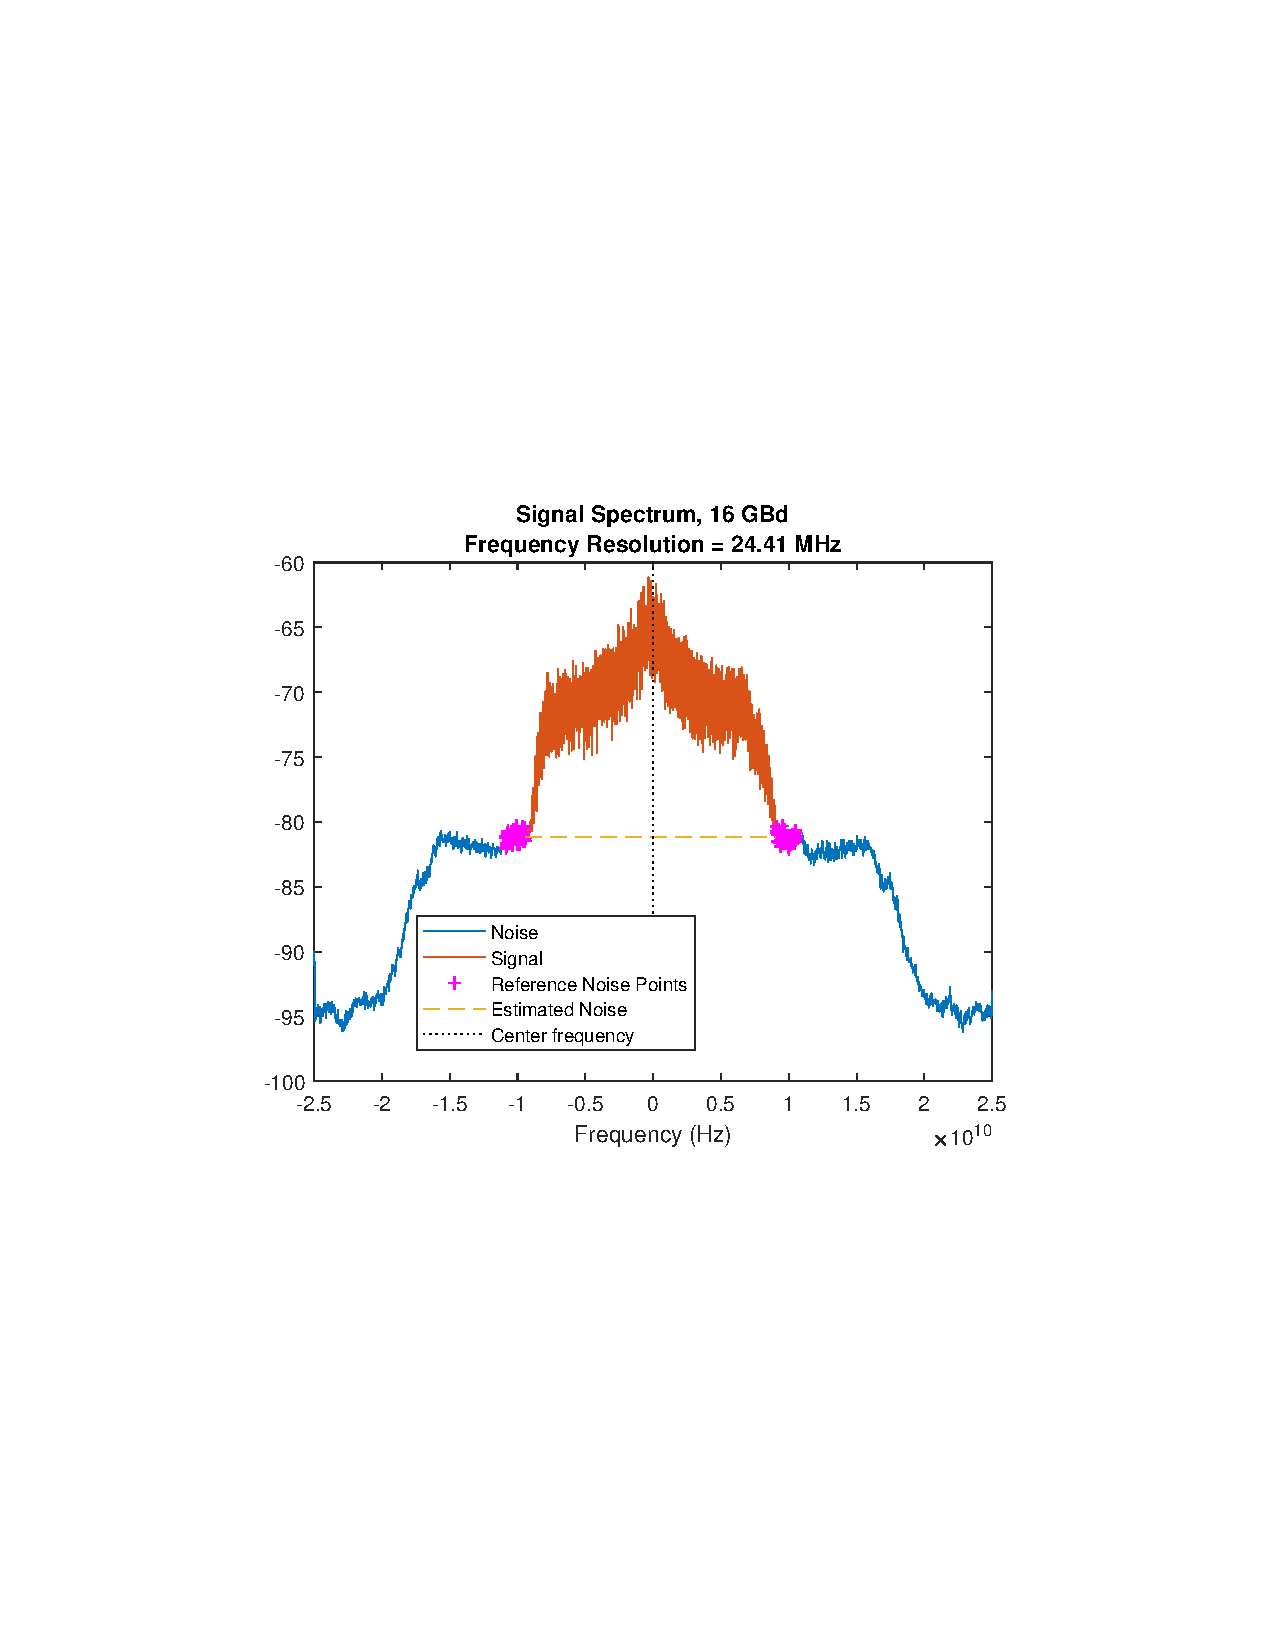
\includegraphics[clip, trim=4cm 8cm 4cm 8cm, width=1\textwidth]{./sdf/m_qam_system/figures/expResults/16GBdSpectrum.pdf}
		
	\subcaption{\label{fig:16GBdSpectrum}}
\end{minipage}
	\caption{Spectrum of the signals obtained at the oscilloscope. The estimated SNR for these signals were 5.7104~dB and 9.4548~dB, for the 4~GBd and 16~GBd signals, respectively.}
\end{figure}

%Figures~\ref{fig:4GBdSpectrum} and~\ref{fig:16GBdSpectrum} show the relation between the estimated SNRs at the input and output of the DSP stack. As mentioned before, the optimum BER curve is proportional to the square root of the peak power SNR. The SNR is itself proportional to $B/S_R$. However, that does not seem to be the exact case here. For 4 and 16 GBd, the ratio $B/S_R$ is equal to 8.25 and 2.06, respectively, considering that the bandwidth is equal to that of the oscilloscope, 33 GHz.
%
%\begin{figure}[H]
%	\begin{minipage}{0.4\textwidth}
%		\centering
%		\textbf{4~GBd}
%		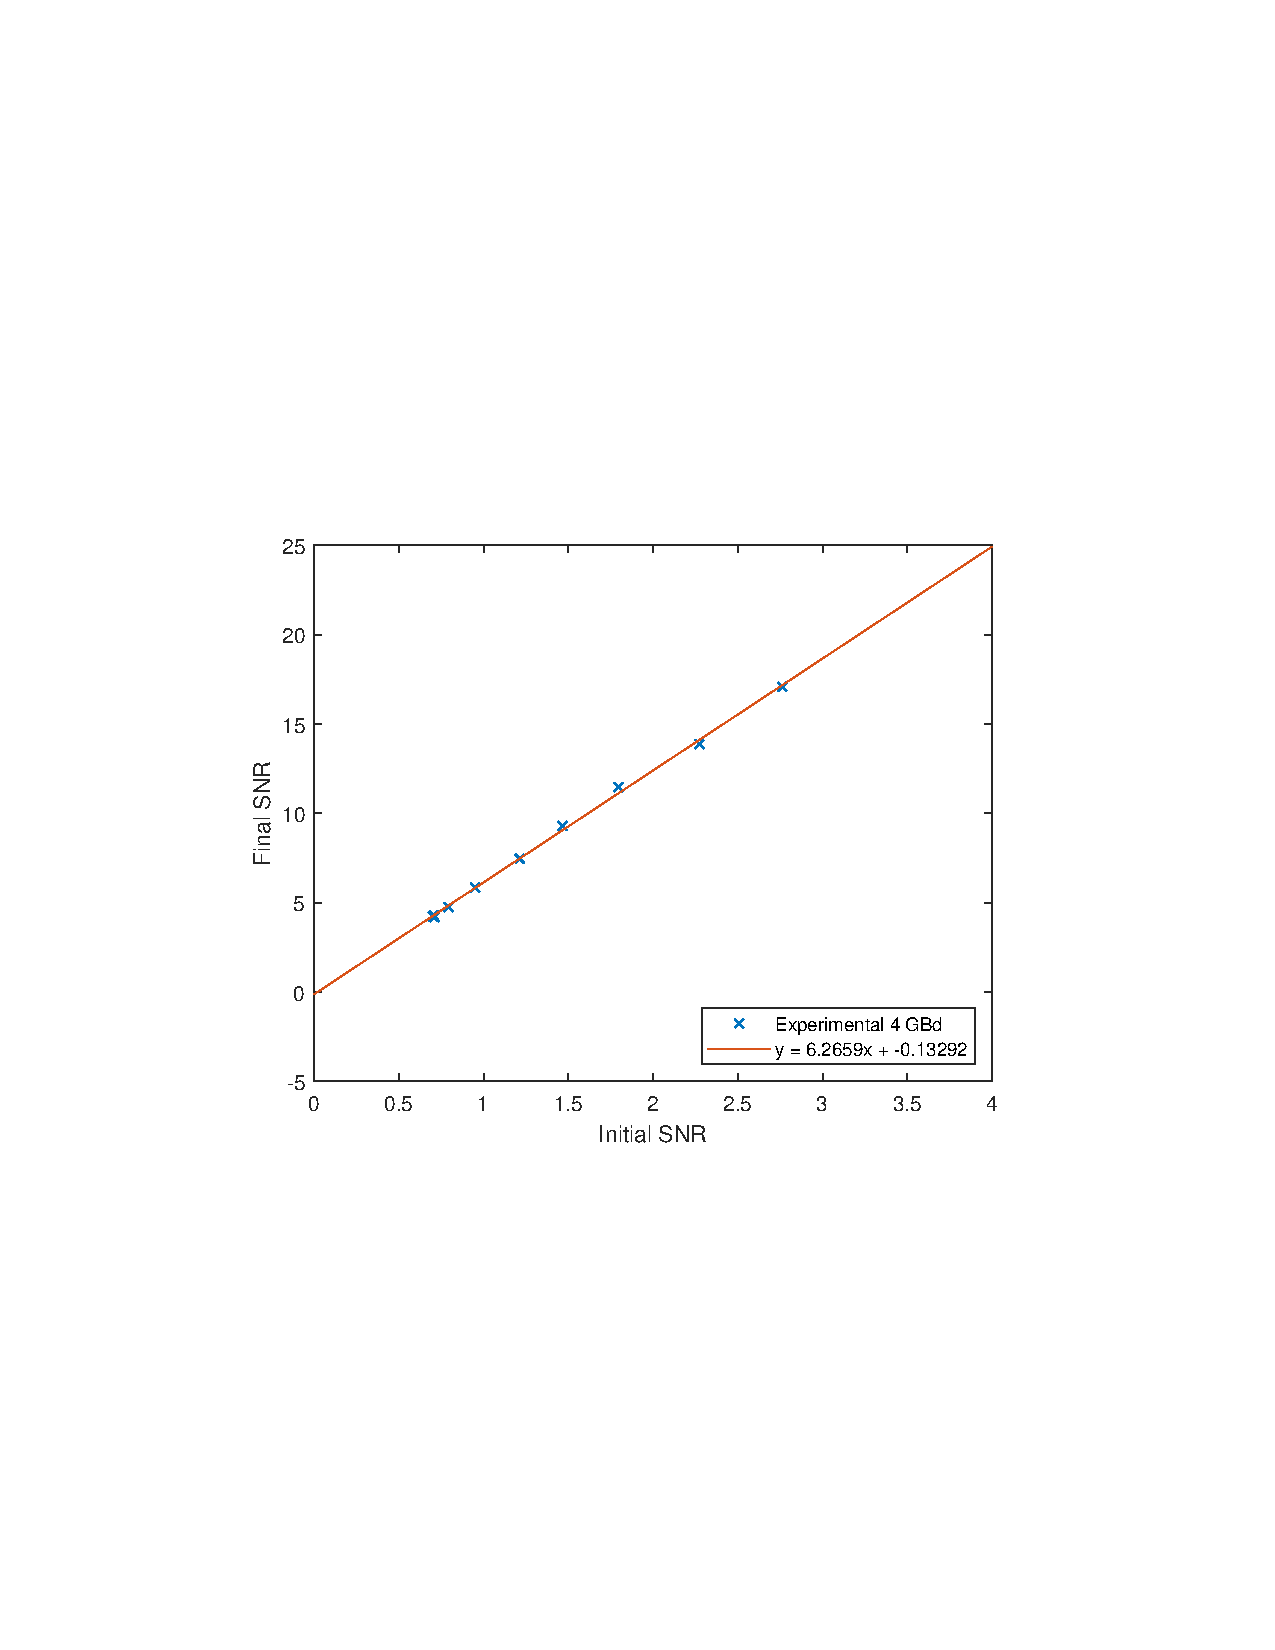
\includegraphics[clip, trim=4cm 8cm 4cm 8cm, width=1\textwidth]{./sdf/m_qam_system/figures/expResults/4GBdSnrVsSnrOut.pdf}
%		\label{fig:snrComp4}
%	\end{minipage}
%	\begin{minipage}{0.4\textwidth}
%		\centering
%		\textbf{16~GBd}
%		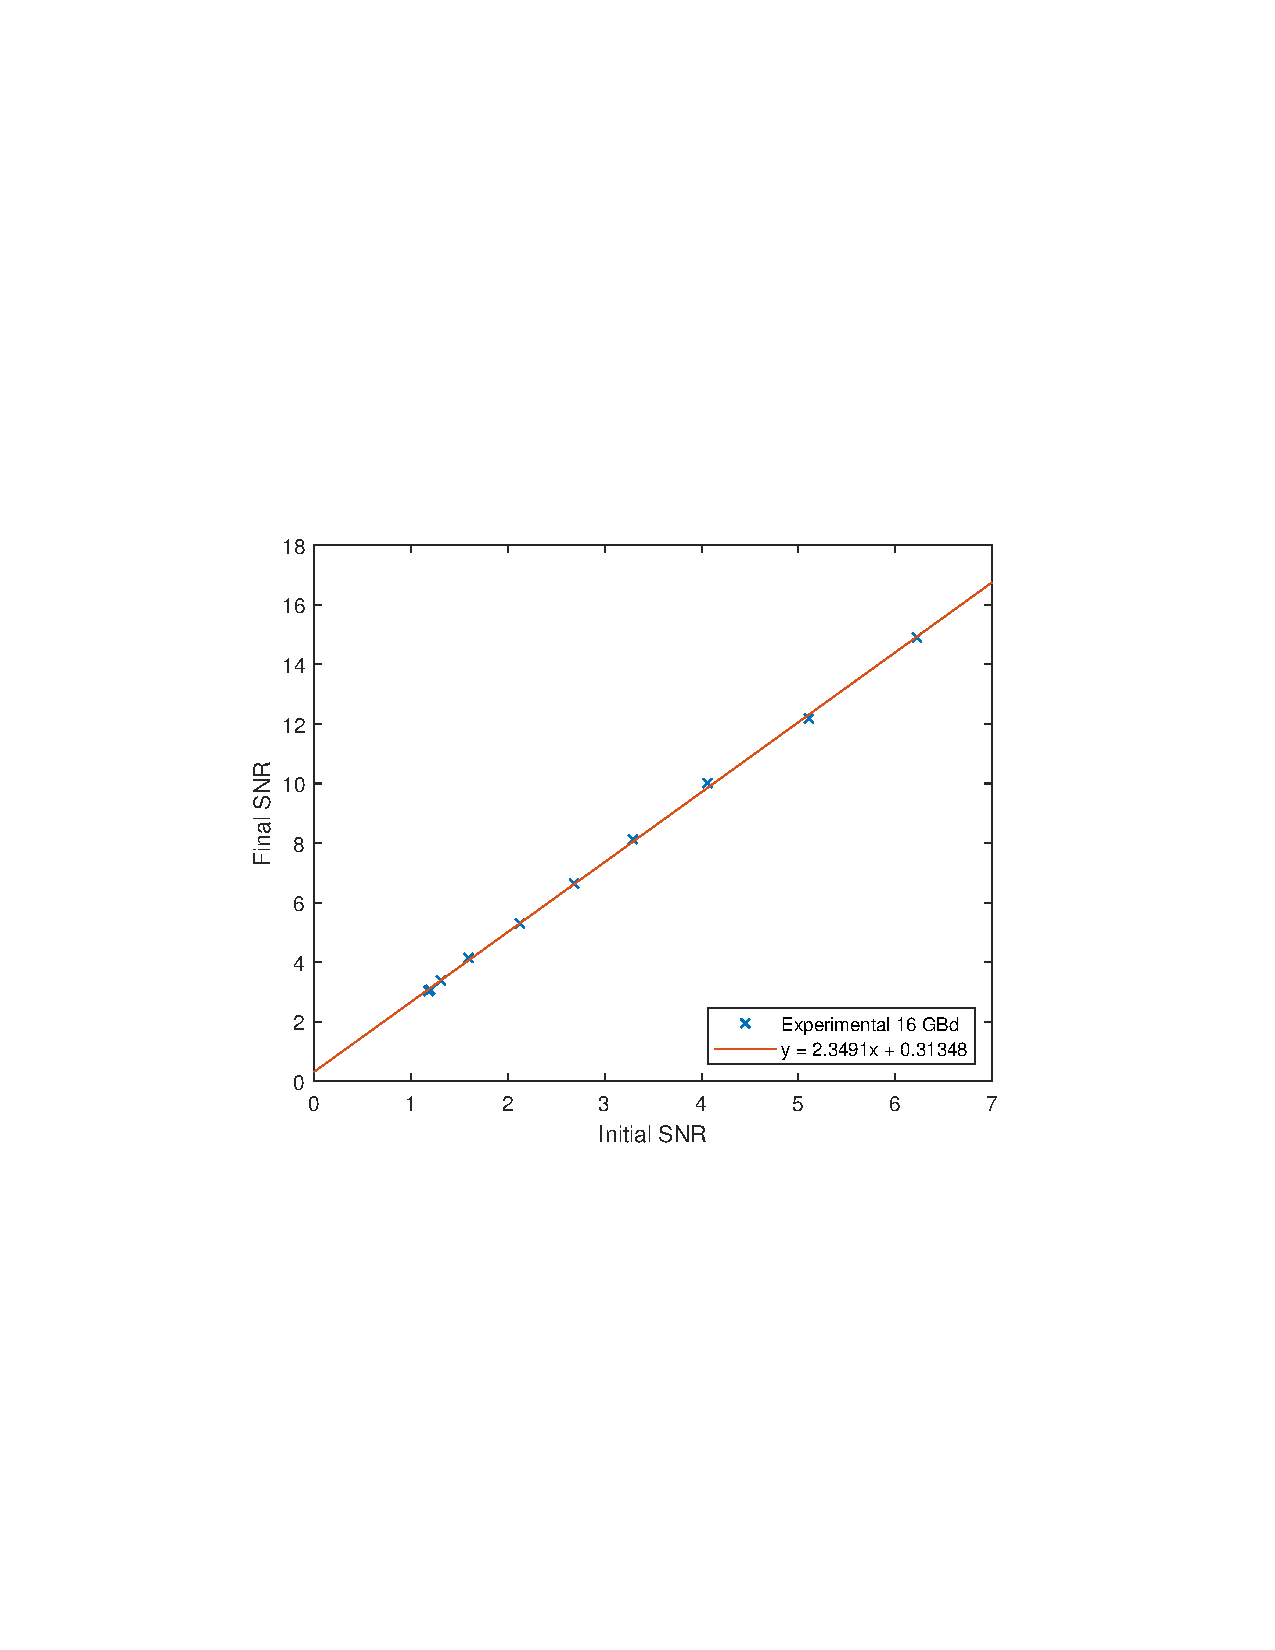
\includegraphics[clip, trim=4cm 8cm 4cm 8cm, width=1\textwidth]{./sdf/m_qam_system/figures/expResults/16GBdSnrVsSnrOut.pdf}
%		\label{fig:snrComp16}
%	\end{minipage}
%	\caption{Relation of the estimated SNR calculated from the oscilloscope's waveform and the final SNR estimated from the final constellation. The SNR values plotted are in the linear domain.}
%\end{figure}

Figure~\ref{fig:expBer} shows the performance for 4~GBd and 16~GBd signals.The 
theoretical curves were obtained resorting to equation~\ref{eq:berMod}.

\begin{figure}[H]
	\centering
	\begin{minipage}{0.43\textwidth}
		\centering
%		\textbf{4~GBd}
		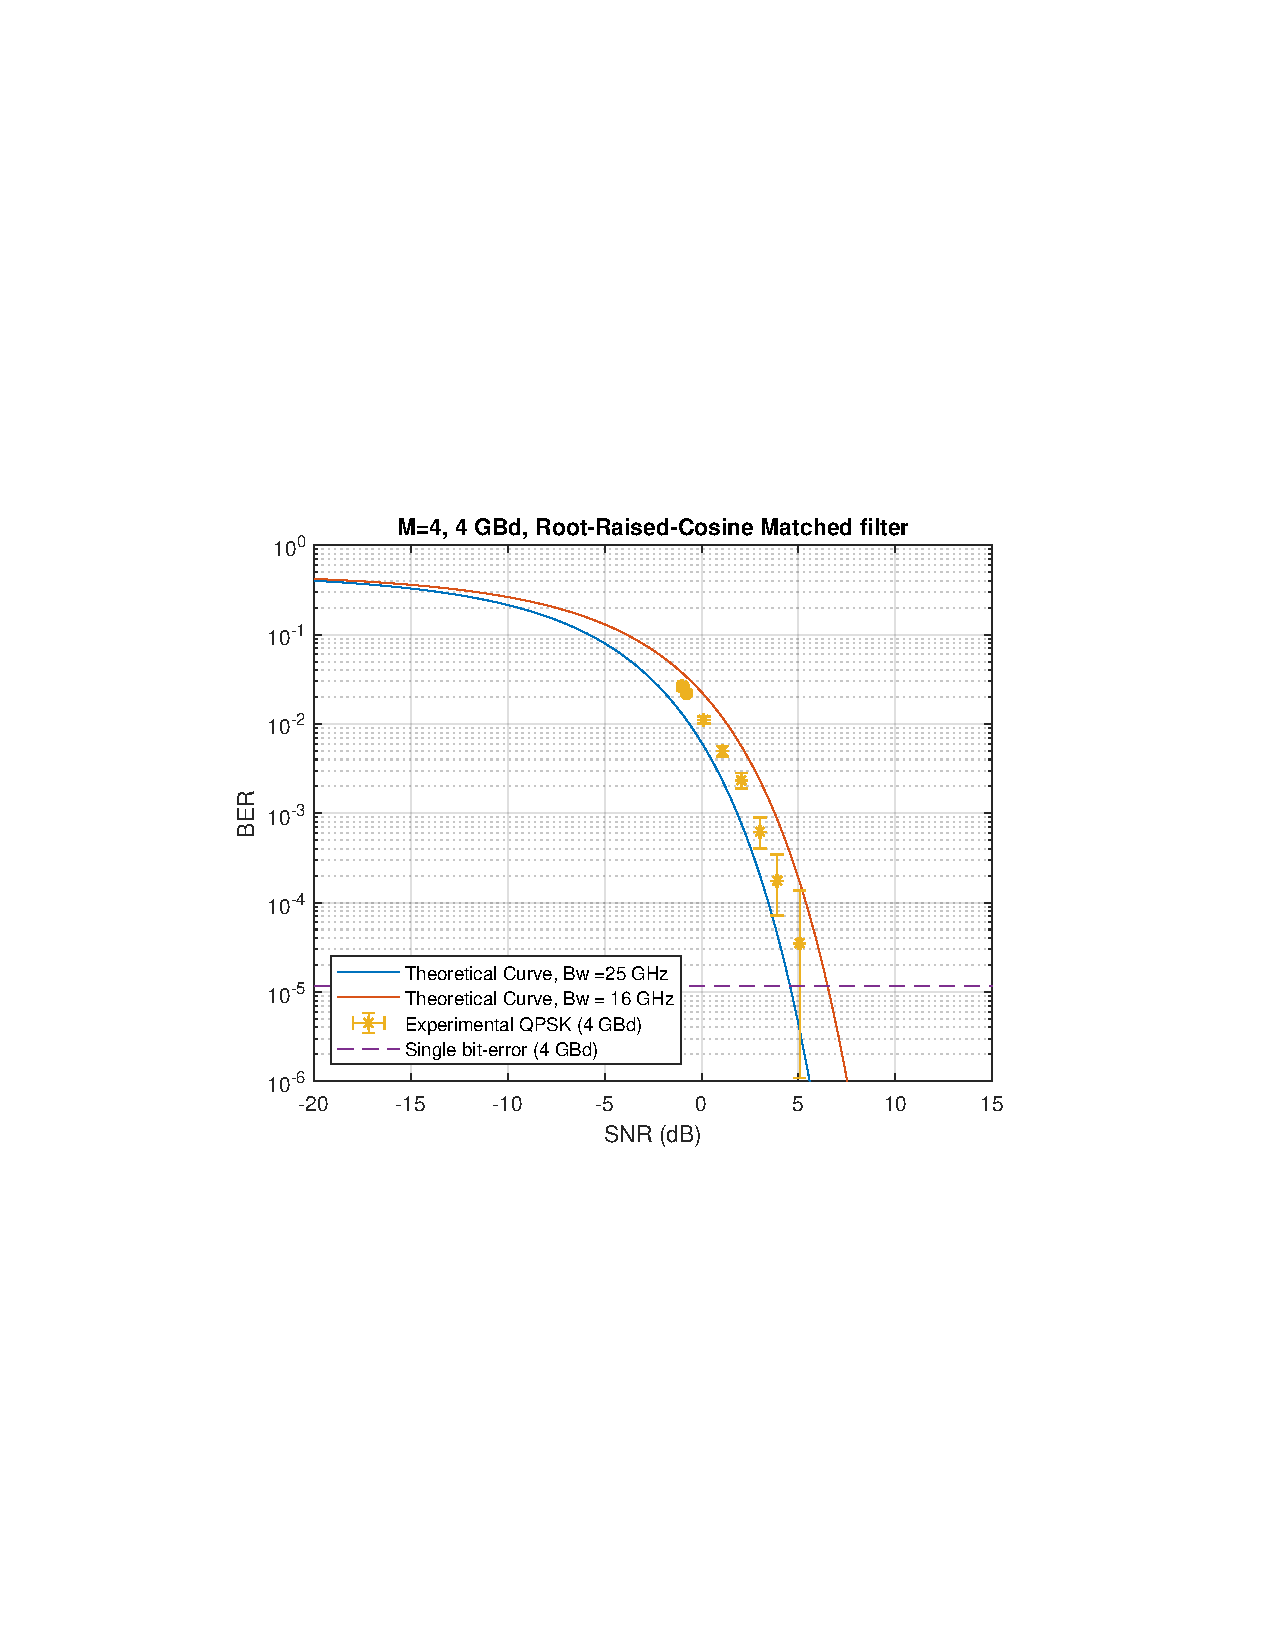
\includegraphics[clip, trim=4cm 8cm 4cm 8cm, width=1\textwidth]{./sdf/m_qam_system/figures/expResults/4GBdBER20180611.pdf}
		\subcaption{\label{fig:4GBdBER}}
	\end{minipage}
	\begin{minipage}{0.43\textwidth}
		\centering
%		\textbf{16~GBd}
		\includegraphics[clip, trim=4cm 8cm 4cm 8cm, width=1\textwidth]{./sdf/m_qam_system/figures/expResults/16GBdBER20180611.pdf}
		\subcaption{\label{fig:16GBdBER}}
	\end{minipage}
	\caption{Comparison of theoretical BER curves against obtained results. SNR 
		values are estimated from the raw waveforms obtained at the oscilloscope, 
		through spectral analysis of the acquired signal. Local oscillator 
		generated at the receiver and frequency deviation compensated by DSP.\label{fig:expBer}}
\end{figure}

%\begin{figure}[H]
%	\centering
%	\includegraphics[clip, trim=4cm 8cm 4cm 8cm, width=0.6\textwidth]{./sdf/m_qam_system/figures/expResults/BerVsSnr_180503.pdf}
%	\caption{Comparison of theoretical BER curves against obtained results. SNR 
%	values are estimated from the raw waveforms obtained at the oscilloscope, 
%	through spectral analysis of the acquired signal. Local oscillator 
%	generated at the receiver and frequency deviation compensated by DSP.}
%	\label{fig:expBer}
%\end{figure}

Figure~\ref{fig:expBerOutSnr} shows the Q-Factor of the signals vs. the 
expected BER. Q-factor is the electrical SNR immediately prior to the decision 
circuit. It shows very good agreement with the expected values, and as such 
can be used to analyze the performance 
when the segment used is not long enough to get low BER values. This can be 
particularly useful for lower baud rates. The equation which relates the Q-factor with the BER is~\cite{ituto201}

\begin{equation}
\text{BER} = \frac{1}{2} \text{erfc}\left( \frac{Q}{\sqrt{2}}\right)
\end{equation}

\begin{figure}[H]
	\centering
	\includegraphics[clip, trim=4cm 8cm 4cm 8cm, 
width=0.6\textwidth]{./sdf/m_qam_system/figures/expResults/qFactorVsBER.pdf}
	\caption{Q-Factor vs BER.}
	\label{fig:expBerOutSnr}
\end{figure}

It can be seen that for values close to the single bit error lines the BER values run away from the theory. However, using the Q-Factor to estimate the BER in these cases can help get a reasonably accurate portrayal of the system performance at lower BERs, particularly for lower sample sizes.

%Figure~\ref{fig:16GBdOptiSnr} shows the relation between BER and SNR of the optical signal. The signal power was calculated by integrating the area of the signal, subtracting the estimated noise that shares the same bandwidth, and dividing by the signal bandwidth. The noise for the SNR was calculated from the remainder of the spectrum, and divided by the full frequency interval of the spectrum.
%
%\begin{figure}[H]
%	\centering
%	\includegraphics[clip, trim=4cm 8cm 4cm 8cm, width=0.6\textwidth]{./sdf/m_qam_system/figures/expResults/BerVsOptSnr.pdf}
%	\caption{SNR measured at the OSA vs measured BER.}
%	\label{fig:expBerOptiSnr}
%\end{figure}


%
\subsubsection{16~GBd Signal}
%
Figure~\ref{fig:16GBdOptiSpect} shows the optical spectrum of a 16~GBd signal. The estimated electrical at the receiver oscilloscope SNR is 9.4548 dB. The signal power was calculated as described in subsection~\ref{ssc:snrEst}, by integrating the area of the signal, subtracting the estimated noise that shares the same bandwidth, and dividing by the estimated signal bandwidth. The noise for the SNR was calculated from the remainder of the spectrum, and divided by the full frequency interval of the spectrum.

\begin{figure}[H]
		\centering
	\begin{minipage}{0.43\textwidth}
	\centering
	\includegraphics[clip, trim=4cm 8cm 4cm 8cm, width=1\textwidth]{./sdf/m_qam_system/figures/expResults/16GBdOSASpectrum.pdf}
	\subcaption{\ref{fig:experimental_mqam_setup}.}
	\label{fig:16GBdOptiSpect}
		\end{minipage}
	\begin{minipage}{0.43\textwidth}
		\centering
		\includegraphics[clip, trim=4cm 8cm 4cm 8cm, width=1\textwidth]{./sdf/m_qam_system/figures/expResults/16GBdSpectrum.pdf}
		\caption{}
		\label{fig:16GBdSpect}
	\end{minipage}
	\caption{Optical and electrical spectra of the transmitted signal, obtained at the OSA ans receiver oscilloscope, at the points shown in Figure~\ref{fig:experimental_mqam_setup}.}
\end{figure}


\begin{figure}[H]
	\centering
	\begin{minipage}{0.30\textwidth}
		\centering
		\includegraphics[clip, trim=4cm 8cm 4cm 8cm, width=1\textwidth]{./sdf/m_qam_system/figures/expResults/intradyne/0_16GBdInSig13dB_bfFec.pdf}
		\label{fig:16GBdEyeBefFec}
	\end{minipage}
	\begin{minipage}{0.30\textwidth}
		\centering
		\includegraphics[clip, trim=4cm 8cm 4cm 8cm, width=1\textwidth]{./sdf/m_qam_system/figures/expResults/intradyne/0_eye_16GBdInSig13dB_bfFec.pdf}
		\label{fig:16GBdSpecBefFec}
	\end{minipage}
	\begin{minipage}{0.30\textwidth}
		\centering
		\includegraphics[clip, trim=4cm 8cm 4cm 8cm, width=1\textwidth]{./sdf/m_qam_system/figures/expResults/intradyne/0_const_16GBdInSig13dB_bfFec.pdf}
		\label{fig:16GBdSpecBefFec}
	\end{minipage}
	\caption{Eye Diagram and spectrum of the original signal obtained at the oscilloscope. Initial estimated SNR before any signal processing is 9.4548 dB.}
	\label{fig:16GBdinit}
\end{figure}

\begin{figure}[H]
	\centering
	\begin{minipage}{0.30\textwidth}
		\centering
		\includegraphics[clip, trim=4cm 8cm 4cm 8cm, width=1\textwidth]{./sdf/m_qam_system/figures/expResults/intradyne/1_16GBdInSig13dB_AfFec.pdf}
		\label{fig:16GBdEyeAftFec}
	\end{minipage}
	\begin{minipage}{0.30\textwidth}
		\centering
		\includegraphics[clip, trim=4cm 8cm 4cm 8cm, width=1\textwidth]{./sdf/m_qam_system/figures/expResults/intradyne/1_eye_16GBdInSig13dB_AfFec.pdf}
		\label{fig:16GBdSpecAftFec}
	\end{minipage}
	\begin{minipage}{0.30\textwidth}
		\centering
		\includegraphics[clip, trim=4cm 8cm 4cm 8cm, width=1\textwidth]{./sdf/m_qam_system/figures/expResults/intradyne/1_const_16GBdInSig13dB_AfFec.pdf}
		\label{fig:16GBdSpecBefFec}
	\end{minipage}
	\caption{Eye Diagram and spectrum after front end corrections, including removal of DC component, deskew and Gram-Schmidt Orthonormalization.}
\end{figure}

\begin{figure}[H]
	\centering
	\begin{minipage}{0.30\textwidth}
		\centering
		\includegraphics[clip, trim=4cm 8cm 4cm 8cm, width=1\textwidth]{./sdf/m_qam_system/figures/expResults/intradyne/2_16GBdInSig13dB_AfMF.pdf}
		\label{fig:16GBdEyeMf}
	\end{minipage}
	\begin{minipage}{0.30\textwidth}
		\centering
		\includegraphics[clip, trim=4cm 8cm 4cm 8cm, width=1\textwidth]{./sdf/m_qam_system/figures/expResults/intradyne/2_eye_16GBdInSig13dB_AfMF.pdf}
		\label{fig:16GBdSpecMF}
	\end{minipage}
	\begin{minipage}{0.30\textwidth}
		\centering
		\includegraphics[clip, trim=4cm 8cm 4cm 8cm, width=1\textwidth]{./sdf/m_qam_system/figures/expResults/intradyne/2_const_16GBdInSig13dB_AfMF.pdf}
		\label{fig:16GBdSpecBefFec}
	\end{minipage}
	\caption{Eye Diagram and spectrum after applying the matched filter and downsampling to $2 S_R$.}
	\label{fig:4GBMF}
\end{figure}

\begin{figure}[H]
	\centering
	\begin{minipage}{0.30\textwidth}
		\centering
		\includegraphics[clip, trim=4cm 8cm 4cm 8cm, width=1\textwidth]{./sdf/m_qam_system/figures/expResults/intradyne/3_16GBdInSig13dB_AfMIMO1.pdf}
		\label{fig:16GBdEyeMIMO1}
	\end{minipage}
	\begin{minipage}{0.30\textwidth}
		\centering
		\includegraphics[clip, trim=4cm 8cm 4cm 8cm, width=1\textwidth]{./sdf/m_qam_system/figures/expResults/intradyne/3_eye_16GBdInSig13dB_AfMIMO1.pdf}
		\label{fig:16GBdSpecMIMO1}
	\end{minipage}
	\begin{minipage}{0.30\textwidth}
		\centering
		\includegraphics[clip, trim=4cm 8cm 4cm 8cm, width=1\textwidth]{./sdf/m_qam_system/figures/expResults/intradyne/3_const_16GBdInSig13dB_AfMIMO1.pdf}
		\label{fig:16GBdSpecBefFec}
	\end{minipage}
	\caption{Eye Diagram and spectrum after the first stage of adaptive equalization, using a MIMO 2x2 CMA equalizer.}
\end{figure}

\begin{figure}[H]
	\centering
	\begin{minipage}{0.30\textwidth}
		\centering
		\includegraphics[clip, trim=4cm 8cm 4cm 8cm, width=1\textwidth]{./sdf/m_qam_system/figures/expResults/intradyne/4_16GBdInSig13dB_AfFE.pdf}
		\label{fig:16GBdEyeFE2}
	\end{minipage}
	\begin{minipage}{0.30\textwidth}
		\centering
		\includegraphics[clip, trim=4cm 8cm 4cm 8cm, width=1\textwidth]{./sdf/m_qam_system/figures/expResults/intradyne/4_eye_16GBdInSig13dB_AfFE.pdf}
		\label{fig:16GBdSpecFE2}
	\end{minipage}
	\begin{minipage}{0.30\textwidth}
		\centering
		\includegraphics[clip, trim=4cm 8cm 4cm 8cm, width=1\textwidth]{./sdf/m_qam_system/figures/expResults/intradyne/4_const_16GBdInSig13dB_AfFE.pdf}
		\label{fig:16GBdSpecBefFec}
	\end{minipage}
	\caption{Eye Diagram and spectrum after frequency offset correction.}
\end{figure}

\begin{figure}[H]
	\centering
	\begin{minipage}{0.30\textwidth}
		\centering
		\includegraphics[clip, trim=4cm 8cm 4cm 8cm, width=1\textwidth]{./sdf/m_qam_system/figures/expResults/intradyne/5_16GBdInSig13dB_AfPE1.pdf}
		\label{fig:16GBdEyePE1}
	\end{minipage}
	\begin{minipage}{0.30\textwidth}
		\centering
		\includegraphics[clip, trim=4cm 8cm 4cm 8cm, width=1\textwidth]{./sdf/m_qam_system/figures/expResults/intradyne/5_eye_16GBdInSig13dB_AfPE.pdf}
		\label{fig:16GBdSpecPE1}
	\end{minipage}
	\begin{minipage}{0.30\textwidth}
		\centering
		\includegraphics[clip, trim=4cm 8cm 4cm 8cm, width=1\textwidth]{./sdf/m_qam_system/figures/expResults/intradyne/5_const_16GBdInSig13dB_AfPE.pdf}
		\label{fig:16GBdSpecBefFec}
	\end{minipage}
	\caption{Eye Diagram and spectrum after the first stage of carrier-phase estimation.}
\end{figure}

\begin{figure}[H]
	\centering
	\begin{minipage}{0.30\textwidth}
		\centering
		\includegraphics[clip, trim=4cm 8cm 4cm 8cm, width=1\textwidth]{./sdf/m_qam_system/figures/expResults/intradyne/6_16GBdInSig13dB_AfMIMO2.pdf}
		\label{fig:16GBdEyeMIMO2}
	\end{minipage}
	\begin{minipage}{0.30\textwidth}
		\centering
		\includegraphics[clip, trim=4cm 8cm 4cm 8cm, width=1\textwidth]{./sdf/m_qam_system/figures/expResults/intradyne/6_eye_16GBdInSig13dB_AfMIMO2.pdf}
		\label{fig:16GBdSpecMIMO2}
	\end{minipage}
	\begin{minipage}{0.30\textwidth}
		\centering
		\includegraphics[clip, trim=4cm 8cm 4cm 8cm, width=1\textwidth]{./sdf/m_qam_system/figures/expResults/intradyne/6_const_16GBdInSig13dB_AfMIMO2.pdf}
		\label{fig:16GBdSpecBefFec}
	\end{minipage}
	\caption{Eye Diagram and spectrum after the second stage of adaptive equalization, with a MIMO 4x4 LMS equalizer.}
\end{figure}

\begin{figure}[H]
	%	\centering
	%	\begin{minipage}{0.40\textwidth}
	%		\centering
	%		\includegraphics[clip, trim=5cm 8cm 5cm 8cm, width=1\textwidth]{./sdf/m_qam_system/figures/expResults/intradyne/7_berCurve.pdf}
	%		\label{fig:16GBdEyePE2}
	%	\end{minipage}
%		\begin{minipage}{0.43\textwidth}
	\centering
	\includegraphics[clip, trim=4cm 8cm 4cm 8cm,
	width=0.7\textwidth]{./sdf/m_qam_system/figures/expResults/intradyne/7_16GBdInSig13dB_const.pdf}
	%		\label{fig:16GBdSpecPE2}
%		\end{minipage}	
	\caption{Final constellation obtained after processing. The BER in this case is $7.62 \times 10^{-5}$.}
	\label{fig:16GBdFinal}
\end{figure}

\begin{figure}[H]
	%	\centering
	%	\begin{minipage}{0.40\textwidth}
	%		\centering
	%		\includegraphics[clip, trim=5cm 8cm 5cm 8cm, width=1\textwidth]{./sdf/m_qam_system/figures/expResults/intradyne/7_berCurve.pdf}
	%		\label{fig:16GBdEyePE2}
	%	\end{minipage}
%			\begin{minipage}{0.43\textwidth}
	\centering
	\includegraphics[clip, trim=4cm 8cm 4cm 8cm,
	width=0.8\textwidth]{./sdf/m_qam_system/figures/expResults/16GBdBER20180611.pdf}
	%		\label{fig:16GBdSpecPE2}
%\end{minipage}	
	\caption{Experimentally obtained BER vs theoretical curve. SNR was estimated as described in Subsection~\ref{ssc:snrEst}.}
	\label{fig:16GBdFinal}
\end{figure}



\subsubsection{4~GBd Signal}
%
Figure~\ref{fig:4GBdOptiSpect} shows the optical spectrum of a 4~GBd signal. The estimated electrical SNR at the receiver oscilloscope is 5.7104 dB. The signal power for the SNR was calculated by integrating the area of the signal, subtracting the estimated noise that shares the same bandwidth, and dividing by the estimated signal bandwidth. The noise for the SNR was calculated by integrating the remainder of the spectrum, interpolating the signal area, and dividing by the full frequency interval of the spectrum.
%%

\begin{figure}[H]
	\centering
	\begin{minipage}{0.43\textwidth}
		\centering
		\includegraphics[clip, trim=4cm 8cm 4cm 8cm, width=1\textwidth]{./sdf/m_qam_system/figures/expResults/4GBdOSASpectrum.pdf}
		\subcaption{\ref{fig:experimental_mqam_setup}.}
		\label{fig:4GBdOptiSpect}
	\end{minipage}
	\begin{minipage}{0.43\textwidth}
		\centering
		\includegraphics[clip, trim=4cm 8cm 4cm 8cm, width=1\textwidth]{./sdf/m_qam_system/figures/expResults/4GBdSpectrum.pdf}
		\caption{}
		\label{fig:4GBdSpect}
	\end{minipage}
	\caption{Optical and electrical spectra of the transmitted signal, obtained at the OSA ans receiver oscilloscope, at the points shown in Figure~\ref{fig:experimental_mqam_setup}.}
\end{figure}



Figures~\ref{fig:4GBdinit} to~\ref{fig:4GBdFinal} show the eye diagrams and the spectrum of the signals at every stage of the DSP process. The process is similar to the described for the 16 GBd signal. However, some differences can be seen, particularly on the signal spectrum before the corrections. A particularly relevant difference is the stronger deviation from the theoretical curve in this case (for ber curve using the SNR calculated at the oscilloscope input), as can be seen in Figure~\ref{fig:expBer}. This can be due to how the SNR is calculated, as it is assumed the signal spectrum is centered in at zero in the frequency domain, and this assumption is not true, as can be seen from the spectrum examples below, particularly in the spectrum of Figure~\ref{fig:4GBMF}.
It is also worth noting that in the input signal the noise is not white. Therefore, the reference points chosen to calculate the noise that shares the frequencies of the signal strongly affect the SNR measurement.
%Although the energy per bit is higher in lower symbol rates, the ratio between linewidth and symbol rate is lower, which affects negatively the performance of the system.

\begin{figure}[H]
	\centering
	\begin{minipage}{0.30\textwidth}
		\centering
		\includegraphics[clip, trim=4cm 8cm 4cm 8cm, width=1\textwidth]{./sdf/m_qam_system/figures/expResults/intradyne/0_4GBdInSig13dB_bfFec.pdf}
		\label{fig:4GBdEyeBefFec}
	\end{minipage}
	\begin{minipage}{0.30\textwidth}
		\centering
		\includegraphics[clip, trim=4cm 8cm 4cm 8cm, width=1\textwidth]{./sdf/m_qam_system/figures/expResults/intradyne/0_eye_4GBdInSig13dB_bfFec.pdf}
		\label{fig:4GBdSpecBefFec}
	\end{minipage}
	\begin{minipage}{0.30\textwidth}
		\centering
		\includegraphics[clip, trim=4cm 8cm 4cm 8cm, width=1\textwidth]{./sdf/m_qam_system/figures/expResults/intradyne/0_const_4GBdInSig13dB_bfFec.pdf}
		\label{fig:4GBdSpecBefFec}
	\end{minipage}
	\caption{Eye Diagram and spectrum of the original signal obtained at the oscilloscope. Initial estimated SNR before any signal processing is 5.7104 dB.}
	\label{fig:4GBdinit}
\end{figure}

\begin{figure}[H]
	\centering
	\begin{minipage}{0.30\textwidth}
		\centering
		\includegraphics[clip, trim=4cm 8cm 4cm 8cm, width=1\textwidth]{./sdf/m_qam_system/figures/expResults/intradyne/1_4GBdInSig13dB_AfFec.pdf}
		\label{fig:4GBdEyeAftFec}
	\end{minipage}
	\begin{minipage}{0.30\textwidth}
		\centering
		\includegraphics[clip, trim=4cm 8cm 4cm 8cm, width=1\textwidth]{./sdf/m_qam_system/figures/expResults/intradyne/1_eye_4GBdInSig13dB_AfFec.pdf}
		\label{fig:4GBdSpecAftFec}
	\end{minipage}
	\begin{minipage}{0.30\textwidth}
		\centering
		\includegraphics[clip, trim=4cm 8cm 4cm 8cm, width=1\textwidth]{./sdf/m_qam_system/figures/expResults/intradyne/1_const_4GBdInSig13dB_AfFec.pdf}
		\label{fig:4GBdSpecBefFec}
	\end{minipage}
	\caption{Eye Diagram and spectrum after front end corrections, including removal of DC component, deskew and Gram-Schmidt Orthonormalization.}
\end{figure}

\begin{figure}[H]
	\centering
	\begin{minipage}{0.30\textwidth}
		\centering
		\includegraphics[clip, trim=4cm 8cm 4cm 8cm, width=1\textwidth]{./sdf/m_qam_system/figures/expResults/intradyne/2_4GBdInSig13dB_AfMF.pdf}
		\label{fig:4GBdEyeMf}
	\end{minipage}
	\begin{minipage}{0.30\textwidth}
		\centering
		\includegraphics[clip, trim=4cm 8cm 4cm 8cm, width=1\textwidth]{./sdf/m_qam_system/figures/expResults/intradyne/2_eye_4GBdInSig13dB_AfMF.pdf}
		\label{fig:4GBdSpecMF}
	\end{minipage}
	\begin{minipage}{0.30\textwidth}
		\centering
		\includegraphics[clip, trim=4cm 8cm 4cm 8cm, width=1\textwidth]{./sdf/m_qam_system/figures/expResults/intradyne/2_const_4GBdInSig13dB_AfMF.pdf}
		\label{fig:4GBdSpecBefFec}
	\end{minipage}
	\caption{Eye Diagram and spectrum after applying the matched filter and resampling to $2 S_R$. The frequency offset is now even more apparent to see, due to the lower sample rate.}
	\label{fig:4GBMF}
\end{figure}

\begin{figure}[H]
	\centering
	\begin{minipage}{0.30\textwidth}
		\centering
		\includegraphics[clip, trim=4cm 8cm 4cm 8cm, width=1\textwidth]{./sdf/m_qam_system/figures/expResults/intradyne/3_4GBdInSig13dB_AfMIMO1.pdf}
		\label{fig:4GBdEyeMIMO1}
	\end{minipage}
	\begin{minipage}{0.30\textwidth}
		\centering
		\includegraphics[clip, trim=4cm 8cm 4cm 8cm, width=1\textwidth]{./sdf/m_qam_system/figures/expResults/intradyne/3_eye_4GBdInSig13dB_AfMIMO1.pdf}
		\label{fig:4GBdSpecMIMO1}
	\end{minipage}
	\begin{minipage}{0.30\textwidth}
		\centering
		\includegraphics[clip, trim=4cm 8cm 4cm 8cm, width=1\textwidth]{./sdf/m_qam_system/figures/expResults/intradyne/3_const_4GBdInSig13dB_AfMIMO1.pdf}
		\label{fig:4GBdSpecBefFec}
	\end{minipage}
	\caption{Eye Diagram and spectrum after the first stage of adaptive equalization, using a MIMO 2x2 CMA equalizer.}
\end{figure}

\begin{figure}[H]
	\centering
	\begin{minipage}{0.30\textwidth}
		\centering
		\includegraphics[clip, trim=4cm 8cm 4cm 8cm, width=1\textwidth]{./sdf/m_qam_system/figures/expResults/intradyne/4_4GBdInSig13dB_AfFE.pdf}
		\label{fig:4GBdEyeFE2}
	\end{minipage}
	\begin{minipage}{0.30\textwidth}
		\centering
		\includegraphics[clip, trim=4cm 8cm 4cm 8cm, width=1\textwidth]{./sdf/m_qam_system/figures/expResults/intradyne/4_eye_4GBdInSig13dB_AfFE.pdf}
		\label{fig:4GBdSpecFE2}
	\end{minipage}
	\begin{minipage}{0.30\textwidth}
		\centering
		\includegraphics[clip, trim=4cm 8cm 4cm 8cm, width=1\textwidth]{./sdf/m_qam_system/figures/expResults/intradyne/4_const_4GBdInSig13dB_AfFE.pdf}
		\label{fig:4GBdSpecBefFec}
	\end{minipage}
	\caption{Eye Diagram and spectrum after frequency offset correction.}
\end{figure}

\begin{figure}[H]
	\centering
	\begin{minipage}{0.30\textwidth}
		\centering
		\includegraphics[clip, trim=4cm 8cm 4cm 8cm, width=1\textwidth]{./sdf/m_qam_system/figures/expResults/intradyne/5_4GBdInSig13dB_AfPE1.pdf}
		\label{fig:4GBdEyePE1}
	\end{minipage}
	\begin{minipage}{0.30\textwidth}
		\centering
		\includegraphics[clip, trim=4cm 8cm 4cm 8cm, width=1\textwidth]{./sdf/m_qam_system/figures/expResults/intradyne/5_eye_4GBdInSig13dB_AfPE.pdf}
		\label{fig:4GBdSpecPE1}
	\end{minipage}
	\begin{minipage}{0.30\textwidth}
		\centering
		\includegraphics[clip, trim=4cm 8cm 4cm 8cm, width=1\textwidth]{./sdf/m_qam_system/figures/expResults/intradyne/5_const_4GBdInSig13dB_AfPE.pdf}
		\label{fig:4GBdSpecBefFec}
	\end{minipage}
	\caption{Eye Diagram and spectrum after the first stage of carrier-phase estimation.}
\end{figure}

\begin{figure}[H]
	\centering
	\begin{minipage}{0.30\textwidth}
		\centering
		\includegraphics[clip, trim=4cm 8cm 4cm 8cm, width=1\textwidth]{./sdf/m_qam_system/figures/expResults/intradyne/6_4GBdInSig13dB_AfMIMO2.pdf}
		\label{fig:4GBdEyeMIMO2}
	\end{minipage}
	\begin{minipage}{0.30\textwidth}
		\centering
		\includegraphics[clip, trim=4cm 8cm 4cm 8cm, width=1\textwidth]{./sdf/m_qam_system/figures/expResults/intradyne/6_eye_4GBdInSig13dB_AfMIMO2.pdf}
		\label{fig:4GBdSpecMIMO2}
	\end{minipage}
	\begin{minipage}{0.30\textwidth}
		\centering
		\includegraphics[clip, trim=4cm 8cm 4cm 8cm, width=1\textwidth]{./sdf/m_qam_system/figures/expResults/intradyne/6_const_4GBdInSig13dB_AfMIMO2.pdf}
		\label{fig:4GBdSpecBefFec}
	\end{minipage}
	\caption{Eye Diagram and spectrum after the second stage of adaptive equalization, with a MIMO 4x4 LMS equalizer.}
\end{figure}

\begin{figure}[H]
	%	\centering
	%	\begin{minipage}{0.40\textwidth}
	%		\centering
	%		\includegraphics[clip, trim=5cm 8cm 5cm 8cm, width=1\textwidth]{./sdf/m_qam_system/figures/expResults/intradyne/7_berCurve.pdf}
	%		\label{fig:4GBdEyePE2}
	%	\end{minipage}
	%		\begin{minipage}{0.43\textwidth}
	\centering
	\includegraphics[clip, trim=4cm 8cm 4cm 8cm,
	width=0.7\textwidth]{./sdf/m_qam_system/figures/expResults/intradyne/7_4GBdInSig13dB_const.pdf}
	%		\label{fig:4GBdSpecPE2}
	%		\end{minipage}	
	\caption{Final constellation obtained after processing. The BER in this case is $7.62 \times 10^{-5}$.}
	\label{fig:4GBdFinal}
\end{figure}

\begin{figure}[H]
	%	\centering
	%	\begin{minipage}{0.40\textwidth}
	%		\centering
	%		\includegraphics[clip, trim=5cm 8cm 5cm 8cm, width=1\textwidth]{./sdf/m_qam_system/figures/expResults/intradyne/7_berCurve.pdf}
	%		\label{fig:4GBdEyePE2}
	%	\end{minipage}
	%			\begin{minipage}{0.43\textwidth}
	\centering
	\includegraphics[clip, trim=4cm 8cm 4cm 8cm,
	width=0.8\textwidth]{./sdf/m_qam_system/figures/expResults/4GBdBER20180611.pdf}
	%		\label{fig:4GBdSpecPE2}
	%\end{minipage}	
	\caption{Experimentally obtained BER vs theoretical curve. SNR was estimated as described in Subsection~\ref{ssc:snrEst}.}
	\label{fig:4GBdFinalBERcurve}
\end{figure}



\subsection{Homodyne Detection}
As the laser source used for transmitting the signal and for act as local oscillator is the same, the frequency is always the same. Therefore, using this configuration there should be no need for frequency estimation or carrier-phase corrections.
\subsection{16 GBd Signal}


%Figure~\ref{fig:4GBdOptiSpect} shows the optical spectrum of a 4~GBd signal. The estimated SNR is 13.0930 dB. The signal power for the SNR was calculated by integrating the area of the signal, subtracting the estimated noise that shares the same bandwidth, and dividing by the estimated signal bandwidth. The noise for the SNR was calculated by integrating the remainder of the spectrum, interpolating the signal area, and dividing by the full frequency interval of the spectrum.
%
%\begin{figure}[H]
%	\centering
%	\includegraphics[clip, trim=4cm 8cm 4cm 8cm, width=0.6\textwidth]{./sdf/m_qam_system/figures/expResults/4GBd13dB_OSASpec.pdf}
%	\caption{Optical spectrum of the transmitted signal, obtained through the OSA, at the point shown in Figure~\ref{fig:experimental_mqam_setup}.}
%	\label{fig:4GBdOptiSpect}
%\end{figure}
%
%Figures~\ref{fig:4GBdinit} to~\ref{fig:4GBdFinal} show the eye diagrams and the spectrum of the signals at every stage of the DSP process. The process is similar to the described for the 16 GBd signal. However, some differences can be seen, particularly on the signal spectrum before the corrections. A particularly relevant difference is the stronger deviation from the theoretical curve in this case (for ber curve using the SNR calculated at the oscilloscope input), as can be seen in Figure~\ref{fig:expBer}. This can be due to how the SNR is calculated, as it is assumed the signal spectrum is centered in at zero in the frequency domain, and this assumption is not true, as can be seen from the spectrum examples below, particularly in the spectrum of Figure~\ref{fig:4GBMF}.
%It is also worth noting that in the input signal the noise is not white. Therefore, the reference points chosen to calculate the noise that shares the frequencies of the signal strongly affect the SNR measurement.
%%Although the energy per bit is higher in lower symbol rates, the ratio between linewidth and symbol rate is lower, which affects negatively the performance of the system.

%
Figure~\ref{fig:16GBdOptiSpect} shows the optical spectrum of a 16~GBd signal. The estimated electrical SNR at the receiver oscilloscope is 8.3329 dB. The signal power for the SNR was calculated as described in section~\ref{ssc:snrEst}.

\begin{figure}[H]
	\centering
	\begin{minipage}{0.43\textwidth}
		\centering
		\includegraphics[clip, trim=4cm 8cm 4cm 8cm, width=1\textwidth]{./sdf/m_qam_system/figures/expResults/homodyne/16GBdOSASpectrum.pdf}
		\subcaption{\ref{fig:experimental_mqam_setup}.}
		\label{fig:16GBdOptiSpectHm}
	\end{minipage}
	\begin{minipage}{0.43\textwidth}
		\centering
		\includegraphics[clip, trim=4cm 8cm 4cm 8cm, width=1\textwidth]{./sdf/m_qam_system/figures/expResults/homodyne/16GBdSpectrum.pdf}
		\caption{}
		\label{fig:16GBdSpectHm}
	\end{minipage}
	\caption{Optical and electrical spectra of the transmitted signal, obtained at the OSA ans receiver oscilloscope, at the points shown in Figure~\ref{fig:experimental_mqam_setup}.}
\end{figure}



Figures~\ref{fig:16GBdinitHm} to~\ref{fig:16GBdFinalHm} show the eye diagrams and the spectrum of the signals at every stage of the DSP process. The process is similar to the described for the intradyne configuration, but without phase or frequency corrections.
%Although the energy per bit is higher in lower symbol rates, the ratio between linewidth and symbol rate is lower, which affects negatively the performance of the system.


\begin{figure}[H]
	\centering
	\begin{minipage}{0.30\textwidth}
		\centering
		\includegraphics[clip, trim=4cm 8cm 4cm 8cm, width=1\textwidth]{./sdf/m_qam_system/figures/expResults/homodyne/0_16GBdInSig13dB_bfFec.pdf}
		\label{fig:16GBdEyeBefFecHm}
	\end{minipage}
	\begin{minipage}{0.30\textwidth}
		\centering
		\includegraphics[clip, trim=4cm 8cm 4cm 8cm, width=1\textwidth]{./sdf/m_qam_system/figures/expResults/homodyne/0_eye_16GBdInSig13dB_bfFec.pdf}
		\label{fig:16GBdSpecBefFecHm}
	\end{minipage}
	\begin{minipage}{0.30\textwidth}
		\centering
		\includegraphics[clip, trim=4cm 8cm 4cm 8cm, width=1\textwidth]{./sdf/m_qam_system/figures/expResults/homodyne/0_const_16GBdInSig13dB_bfFec.pdf}
		\label{fig:16GBdSpecBefFecCHm}
	\end{minipage}
	\caption{Eye Diagram and spectrum of the original signal obtained at the oscilloscope. Initial estimated SNR before any signal processing is 8.3329 dB.}
	\label{fig:16GBdinitHm}
\end{figure}

\begin{figure}[H]
	\centering
	\begin{minipage}{0.30\textwidth}
		\centering
		\includegraphics[clip, trim=4cm 8cm 4cm 8cm, width=1\textwidth]{./sdf/m_qam_system/figures/expResults/homodyne/1_16GBdInSig13dB_AfFec.pdf}
		\label{fig:16GBdEyeAftFec}
	\end{minipage}
	\begin{minipage}{0.30\textwidth}
		\centering
		\includegraphics[clip, trim=4cm 8cm 4cm 8cm, width=1\textwidth]{./sdf/m_qam_system/figures/expResults/homodyne/1_eye_16GBdInSig13dB_AfFec.pdf}
		\label{fig:16GBdSpecAftFec}
	\end{minipage}
	\begin{minipage}{0.30\textwidth}
		\centering
		\includegraphics[clip, trim=4cm 8cm 4cm 8cm, width=1\textwidth]{./sdf/m_qam_system/figures/expResults/homodyne/1_const_16GBdInSig13dB_AfFec.pdf}
		\label{fig:16GBdSpecBefFec}
	\end{minipage}
	\caption{Eye Diagram and spectrum after front end corrections, including removal of DC component, deskew and Gram-Schmidt Orthonormalization.}
\end{figure}

\begin{figure}[H]
	\centering
	\begin{minipage}{0.30\textwidth}
		\centering
		\includegraphics[clip, trim=4cm 8cm 4cm 8cm, width=1\textwidth]{./sdf/m_qam_system/figures/expResults/homodyne/2_16GBdInSig13dB_AfMF.pdf}
		\label{fig:16GBdEyeMf}
	\end{minipage}
	\begin{minipage}{0.30\textwidth}
		\centering
		\includegraphics[clip, trim=4cm 8cm 4cm 8cm, width=1\textwidth]{./sdf/m_qam_system/figures/expResults/homodyne/2_eye_16GBdInSig13dB_AfMF.pdf}
		\label{fig:16GBdSpecMF}
	\end{minipage}
	\begin{minipage}{0.30\textwidth}
		\centering
		\includegraphics[clip, trim=4cm 8cm 4cm 8cm, width=1\textwidth]{./sdf/m_qam_system/figures/expResults/homodyne/2_const_16GBdInSig13dB_AfMF.pdf}
		\label{fig:16GBdSpecBefFec}
	\end{minipage}
	\caption{Eye Diagram and spectrum after applying the matched filter and resampling to $2 S_R$.}
	\label{fig:16GBMFHm}
\end{figure}

\begin{figure}[H]
	\centering
	\begin{minipage}{0.30\textwidth}
		\centering
		\includegraphics[clip, trim=4cm 8cm 4cm 8cm, width=1\textwidth]{./sdf/m_qam_system/figures/expResults/homodyne/3_16GBdInSig13dB_AfMIMO1.pdf}
		\label{fig:16GBdEyeMIMO1}
	\end{minipage}
	\begin{minipage}{0.30\textwidth}
		\centering
		\includegraphics[clip, trim=4cm 8cm 4cm 8cm, width=1\textwidth]{./sdf/m_qam_system/figures/expResults/homodyne/3_eye_16GBdInSig13dB_AfMIMO1.pdf}
		\label{fig:16GBdSpecMIMO1}
	\end{minipage}
	\begin{minipage}{0.30\textwidth}
		\centering
		\includegraphics[clip, trim=4cm 8cm 4cm 8cm, width=1\textwidth]{./sdf/m_qam_system/figures/expResults/homodyne/3_const_16GBdInSig13dB_AfMIMO1.pdf}
		\label{fig:16GBdSpecBefFec}
	\end{minipage}
	\caption{Eye Diagram and spectrum after the first stage of adaptive equalization, using a MIMO 2x2 CMA equalizer.}
\end{figure}


\begin{figure}[H]
	\centering
	\begin{minipage}{0.30\textwidth}
		\centering
		\includegraphics[clip, trim=4cm 8cm 4cm 8cm, width=1\textwidth]{./sdf/m_qam_system/figures/expResults/homodyne/5_16GBdInSig13dB_AfMIMO2.pdf}
		\label{fig:16GBdEyeMIMO2}
	\end{minipage}
	\begin{minipage}{0.30\textwidth}
		\centering
		\includegraphics[clip, trim=4cm 8cm 4cm 8cm, width=1\textwidth]{./sdf/m_qam_system/figures/expResults/homodyne/5_eye_16GBdInSig13dB_AfMIMO2.pdf}
		\label{fig:16GBdSpecMIMO2}
	\end{minipage}
	\begin{minipage}{0.30\textwidth}
		\centering
		\includegraphics[clip, trim=4cm 8cm 4cm 8cm, width=1\textwidth]{./sdf/m_qam_system/figures/expResults/homodyne/5_const_16GBdInSig13dB_AfMIMO2.pdf}
		\label{fig:16GBdSpecBefFec}
	\end{minipage}
	\caption{Eye Diagram and spectrum after the second stage of adaptive equalization, with a MIMO 4x4 LMS equalizer.}
\end{figure}

\begin{figure}[H]
	%	\centering
	%	\begin{minipage}{0.40\textwidth}
	%		\centering
	%		\includegraphics[clip, trim=5cm 8cm 5cm 8cm, width=1\textwidth]{./sdf/m_qam_system/figures/expResults/homodyne/7_berCurve.pdf}
	%		\label{fig:16GBdEyePE2}
	%	\end{minipage}
	%		\begin{minipage}{0.43\textwidth}
	\centering
	\includegraphics[clip, trim=4cm 8cm 4cm 8cm,
	width=0.7\textwidth]{./sdf/m_qam_system/figures/expResults/homodyne/6_16GBdInSig13dB_const.pdf}
	%		\label{fig:16GBdSpecPE2}
	%		\end{minipage}	
	\caption{Final constellation obtained after processing. The BER in this case is $6.85 \times 10^{-4}$.}
	\label{fig:16GBdFinalHm}
\end{figure}

\begin{figure}[H]
	%	\centering
	%	\begin{minipage}{0.40\textwidth}
	%		\centering
	%		\includegraphics[clip, trim=5cm 8cm 5cm 8cm, width=1\textwidth]{./sdf/m_qam_system/figures/expResults/homodyne/7_berCurve.pdf}
	%		\label{fig:4GBdEyePE2}
	%	\end{minipage}
	%			\begin{minipage}{0.43\textwidth}
	\centering
	\includegraphics[clip, trim=4cm 8cm 4cm 8cm,
	width=0.8\textwidth]{./sdf/m_qam_system/figures/expResults/homodyne/16GBdBER20180611.pdf}
	%		\label{fig:16GBdSpecPE2}
	%\end{minipage}	
	\caption{Experimentally obtained BER vs theoretical curve. SNR was estimated as described in Subsection~\ref{ssc:snrEst}.}
	\label{fig:16GBdFinalBERcurveHm}
\end{figure}




\subsubsection{4~GBd Signal}


%Figure~\ref{fig:4GBdOptiSpect} shows the optical spectrum of a 4~GBd signal. The estimated SNR is 13.0930 dB. The signal power for the SNR was calculated by integrating the area of the signal, subtracting the estimated noise that shares the same bandwidth, and dividing by the estimated signal bandwidth. The noise for the SNR was calculated by integrating the remainder of the spectrum, interpolating the signal area, and dividing by the full frequency interval of the spectrum.
%
%\begin{figure}[H]
%	\centering
%	\includegraphics[clip, trim=4cm 8cm 4cm 8cm, width=0.6\textwidth]{./sdf/m_qam_system/figures/expResults/4GBd13dB_OSASpec.pdf}
%	\caption{Optical spectrum of the transmitted signal, obtained through the OSA, at the point shown in Figure~\ref{fig:experimental_mqam_setup}.}
%	\label{fig:4GBdOptiSpect}
%\end{figure}
%
%Figures~\ref{fig:4GBdinit} to~\ref{fig:4GBdFinal} show the eye diagrams and the spectrum of the signals at every stage of the DSP process. The process is similar to the described for the 16 GBd signal. However, some differences can be seen, particularly on the signal spectrum before the corrections. A particularly relevant difference is the stronger deviation from the theoretical curve in this case (for ber curve using the SNR calculated at the oscilloscope input), as can be seen in Figure~\ref{fig:expBer}. This can be due to how the SNR is calculated, as it is assumed the signal spectrum is centered in at zero in the frequency domain, and this assumption is not true, as can be seen from the spectrum examples below, particularly in the spectrum of Figure~\ref{fig:4GBMF}.
%It is also worth noting that in the input signal the noise is not white. Therefore, the reference points chosen to calculate the noise that shares the frequencies of the signal strongly affect the SNR measurement.
%%Although the energy per bit is higher in lower symbol rates, the ratio between linewidth and symbol rate is lower, which affects negatively the performance of the system.

%
This section is similar as the one for the 16GBd signal with homodyne receiver.
Figure~\ref{fig:4GBdOptiSpect} shows the optical spectrum of the 4~GBd signal. The estimated electrical SNR at the receiver oscilloscope is 4.9094 dB. The SNR was calculated as described in section~\ref{ssc:snrEst}.
%%

\begin{figure}[H]
	\centering
	\begin{minipage}{0.43\textwidth}
		\centering
		\includegraphics[clip, trim=4cm 8cm 4cm 8cm, width=1\textwidth]{./sdf/m_qam_system/figures/expResults/homodyne/4GBdOSASpectrum.pdf}
		\subcaption{\ref{fig:experimental_mqam_setup}.}
		\label{fig:4GBdOptiSpectHm}
	\end{minipage}
	\begin{minipage}{0.43\textwidth}
		\centering
		\includegraphics[clip, trim=4cm 8cm 4cm 8cm, width=1\textwidth]{./sdf/m_qam_system/figures/expResults/homodyne/4GBdSpectrum.pdf}
		\caption{}
		\label{fig:4GBdSpectHm}
	\end{minipage}
	\caption{Optical and electrical spectra of the transmitted signal, obtained at the OSA ans receiver oscilloscope, at the points shown in Figure~\ref{fig:experimental_mqam_setup}.}
\end{figure}



Figures~\ref{fig:4GBdinitHm} to~\ref{fig:4GBdFinalHm} show the eye diagrams and the spectrum of the signals at every stage of the DSP process. The process is similar to the described for the 16 GBd signal with homodyne receiver. However, some differences can be seen, particularly on the signal spectrum before the corrections. However, it can be seen that the distribution of points in the final constellation is not optimal, unlike in the 16~GBd case.
%Although the energy per bit is higher in lower symbol rates, the ratio between linewidth and symbol rate is lower, which affects negatively the performance of the system.


\begin{figure}[H]
	\centering
	\begin{minipage}{0.30\textwidth}
		\centering
		\includegraphics[clip, trim=4cm 8cm 4cm 8cm, width=1\textwidth]{./sdf/m_qam_system/figures/expResults/homodyne/0_4GBdInSig13dB_bfFec.pdf}
		\label{fig:4GBdEyeBefFecHm}
	\end{minipage}
	\begin{minipage}{0.30\textwidth}
		\centering
		\includegraphics[clip, trim=4cm 8cm 4cm 8cm, width=1\textwidth]{./sdf/m_qam_system/figures/expResults/homodyne/0_eye_4GBdInSig13dB_bfFec.pdf}
		\label{fig:4GBdSpecBefFecHm}
	\end{minipage}
	\begin{minipage}{0.30\textwidth}
		\centering
		\includegraphics[clip, trim=4cm 8cm 4cm 8cm, width=1\textwidth]{./sdf/m_qam_system/figures/expResults/homodyne/0_const_4GBdInSig13dB_bfFec.pdf}
		\label{fig:4GBdSpecBefFecCHm}
	\end{minipage}
	\caption{Eye Diagram and spectrum of the original signal obtained at the oscilloscope. Initial estimated SNR before any signal processing is 4.9094 dB.}
	\label{fig:4GBdinitHm}
\end{figure}

\begin{figure}[H]
	\centering
	\begin{minipage}{0.30\textwidth}
		\centering
		\includegraphics[clip, trim=4cm 8cm 4cm 8cm, width=1\textwidth]{./sdf/m_qam_system/figures/expResults/homodyne/1_4GBdInSig13dB_AfFec.pdf}
		\label{fig:4GBdEyeAftFec}
	\end{minipage}
	\begin{minipage}{0.30\textwidth}
		\centering
		\includegraphics[clip, trim=4cm 8cm 4cm 8cm, width=1\textwidth]{./sdf/m_qam_system/figures/expResults/homodyne/1_eye_4GBdInSig13dB_AfFec.pdf}
		\label{fig:4GBdSpecAftFec}
	\end{minipage}
	\begin{minipage}{0.30\textwidth}
		\centering
		\includegraphics[clip, trim=4cm 8cm 4cm 8cm, width=1\textwidth]{./sdf/m_qam_system/figures/expResults/homodyne/1_const_4GBdInSig13dB_AfFec.pdf}
		\label{fig:4GBdSpecBefFec}
	\end{minipage}
	\caption{Eye Diagram and spectrum after front end corrections, including removal of DC component, deskew and Gram-Schmidt Orthonormalization.}
\end{figure}

\begin{figure}[H]
	\centering
	\begin{minipage}{0.30\textwidth}
		\centering
		\includegraphics[clip, trim=4cm 8cm 4cm 8cm, width=1\textwidth]{./sdf/m_qam_system/figures/expResults/homodyne/2_4GBdInSig13dB_AfMF.pdf}
		\label{fig:4GBdEyeMf}
	\end{minipage}
	\begin{minipage}{0.30\textwidth}
		\centering
		\includegraphics[clip, trim=4cm 8cm 4cm 8cm, width=1\textwidth]{./sdf/m_qam_system/figures/expResults/homodyne/2_eye_4GBdInSig13dB_AfMF.pdf}
		\label{fig:4GBdSpecMF}
	\end{minipage}
	\begin{minipage}{0.30\textwidth}
		\centering
		\includegraphics[clip, trim=4cm 8cm 4cm 8cm, width=1\textwidth]{./sdf/m_qam_system/figures/expResults/homodyne/2_const_4GBdInSig13dB_AfMF.pdf}
		\label{fig:4GBdSpecBefFec}
	\end{minipage}
	\caption{Eye Diagram and spectrum after applying the matched filter and resampling to $2 S_R$.}
	\label{fig:4GBMFHm}
\end{figure}

\begin{figure}[H]
	\centering
	\begin{minipage}{0.30\textwidth}
		\centering
		\includegraphics[clip, trim=4cm 8cm 4cm 8cm, width=1\textwidth]{./sdf/m_qam_system/figures/expResults/homodyne/3_4GBdInSig13dB_AfMIMO1.pdf}
		\label{fig:4GBdEyeMIMO1}
	\end{minipage}
	\begin{minipage}{0.30\textwidth}
		\centering
		\includegraphics[clip, trim=4cm 8cm 4cm 8cm, width=1\textwidth]{./sdf/m_qam_system/figures/expResults/homodyne/3_eye_4GBdInSig13dB_AfMIMO1.pdf}
		\label{fig:4GBdSpecMIMO1}
	\end{minipage}
	\begin{minipage}{0.30\textwidth}
		\centering
		\includegraphics[clip, trim=4cm 8cm 4cm 8cm, width=1\textwidth]{./sdf/m_qam_system/figures/expResults/homodyne/3_const_4GBdInSig13dB_AfMIMO1.pdf}
		\label{fig:4GBdSpecBefFec}
	\end{minipage}
	\caption{Eye Diagram and spectrum after the first stage of adaptive equalization, using a MIMO 2x2 CMA equalizer.}
\end{figure}


\begin{figure}[H]
	\centering
	\begin{minipage}{0.30\textwidth}
		\centering
		\includegraphics[clip, trim=4cm 8cm 4cm 8cm, width=1\textwidth]{./sdf/m_qam_system/figures/expResults/homodyne/5_4GBdInSig13dB_AfMIMO2.pdf}
		\label{fig:4GBdEyeMIMO2}
	\end{minipage}
	\begin{minipage}{0.30\textwidth}
		\centering
		\includegraphics[clip, trim=4cm 8cm 4cm 8cm, width=1\textwidth]{./sdf/m_qam_system/figures/expResults/homodyne/5_eye_4GBdInSig13dB_AfMIMO2.pdf}
		\label{fig:4GBdSpecMIMO2}
	\end{minipage}
	\begin{minipage}{0.30\textwidth}
		\centering
		\includegraphics[clip, trim=4cm 8cm 4cm 8cm, width=1\textwidth]{./sdf/m_qam_system/figures/expResults/homodyne/5_const_4GBdInSig13dB_AfMIMO2.pdf}
		\label{fig:4GBdSpecBefFec}
	\end{minipage}
	\caption{Eye Diagram and spectrum after the second stage of adaptive equalization, with a MIMO 4x4 LMS equalizer.}
\end{figure}

\begin{figure}[H]
	%	\centering
	%	\begin{minipage}{0.40\textwidth}
	%		\centering
	%		\includegraphics[clip, trim=5cm 8cm 5cm 8cm, width=1\textwidth]{./sdf/m_qam_system/figures/expResults/homodyne/7_berCurve.pdf}
	%		\label{fig:4GBdEyePE2}
	%	\end{minipage}
	%		\begin{minipage}{0.43\textwidth}
	\centering
	\includegraphics[clip, trim=4cm 8cm 4cm 8cm,
	width=0.7\textwidth]{./sdf/m_qam_system/figures/expResults/homodyne/6_4GBdInSig13dB_const.pdf}
	%		\label{fig:4GBdSpecPE2}
	%		\end{minipage}	
	\caption{Final constellation obtained after processing. The BER in this case is $3.037525 \times 10^{-4}$.}
	\label{fig:4GBdFinalHm}
\end{figure}

\begin{figure}[H]
	%	\centering
	%	\begin{minipage}{0.40\textwidth}
	%		\centering
	%		\includegraphics[clip, trim=5cm 8cm 5cm 8cm, width=1\textwidth]{./sdf/m_qam_system/figures/expResults/homodyne/7_berCurve.pdf}
	%		\label{fig:4GBdEyePE2}
	%	\end{minipage}
	%			\begin{minipage}{0.43\textwidth}
	\centering
	\includegraphics[clip, trim=4cm 8cm 4cm 8cm,
	width=0.8\textwidth]{./sdf/m_qam_system/figures/expResults/homodyne/4GBdBERNoComp20180611.pdf}
	%		\label{fig:4GBdSpecPE2}
	%\end{minipage}	
	\caption{Experimentally obtained BER vs theoretical curve. SNR was estimated as described in Subsection~\ref{ssc:snrEst}.}
	\label{fig:4GBdFinalBERcurveHm}
\end{figure}


\subsubsection{4 GBd signal, with frequency and phase corrections}

In order to try improving results, the same DSP process used with the intradyne receiver was tested with this for this signal. It can be seen that results were still  improved, benefiting from the frequency and phase offset corrections, even though a homodyne configuration was used for receiving the signal. 


\begin{figure}[H]
	\centering
	\begin{minipage}{0.30\textwidth}
		\centering
		\includegraphics[clip, trim=4cm 8cm 4cm 8cm, width=1\textwidth]{./sdf/m_qam_system/figures/expResults/homodyne/0_4GBdInSig13dBc_bfFec.pdf}
		\label{fig:4GBdEyeBefFecHm}
	\end{minipage}
	\begin{minipage}{0.30\textwidth}
		\centering
		\includegraphics[clip, trim=4cm 8cm 4cm 8cm, width=1\textwidth]{./sdf/m_qam_system/figures/expResults/homodyne/0_eye_4GBdInSig13dBc_bfFec.pdf}
		\label{fig:4GBdSpecBefFecHm}
	\end{minipage}
	\begin{minipage}{0.30\textwidth}
		\centering
		\includegraphics[clip, trim=4cm 8cm 4cm 8cm, width=1\textwidth]{./sdf/m_qam_system/figures/expResults/homodyne/0_const_4GBdInSig13dBc_bfFec.pdf}
		\label{fig:4GBdSpecBefFecCHm}
	\end{minipage}
	\caption{Eye Diagram and spectrum of the original signal obtained at the oscilloscope. Initial estimated SNR before any signal processing is 4.9094 dB.}
	\label{fig:4GBdinitHm}
\end{figure}

\begin{figure}[H]
	\centering
	\begin{minipage}{0.30\textwidth}
		\centering
		\includegraphics[clip, trim=4cm 8cm 4cm 8cm, width=1\textwidth]{./sdf/m_qam_system/figures/expResults/homodyne/1_4GBdInSig13dBc_AfFec.pdf}
		\label{fig:4GBdEyeAftFec}
	\end{minipage}
	\begin{minipage}{0.30\textwidth}
		\centering
		\includegraphics[clip, trim=4cm 8cm 4cm 8cm, width=1\textwidth]{./sdf/m_qam_system/figures/expResults/homodyne/1_eye_4GBdInSig13dBc_AfFec.pdf}
		\label{fig:4GBdSpecAftFec}
	\end{minipage}
	\begin{minipage}{0.30\textwidth}
		\centering
		\includegraphics[clip, trim=4cm 8cm 4cm 8cm, width=1\textwidth]{./sdf/m_qam_system/figures/expResults/homodyne/1_const_4GBdInSig13dBc_AfFec.pdf}
		\label{fig:4GBdSpecBefFec}
	\end{minipage}
	\caption{Eye Diagram and spectrum after front end corrections, including removal of DC component, deskew and Gram-Schmidt Orthonormalization.}
\end{figure}

\begin{figure}[H]
	\centering
	\begin{minipage}{0.30\textwidth}
		\centering
		\includegraphics[clip, trim=4cm 8cm 4cm 8cm, width=1\textwidth]{./sdf/m_qam_system/figures/expResults/homodyne/2_4GBdInSig13dBc_AfMF.pdf}
		\label{fig:4GBdEyeMf}
	\end{minipage}
	\begin{minipage}{0.30\textwidth}
		\centering
		\includegraphics[clip, trim=4cm 8cm 4cm 8cm, width=1\textwidth]{./sdf/m_qam_system/figures/expResults/homodyne/2_eye_4GBdInSig13dBc_AfMF.pdf}
		\label{fig:4GBdSpecMF}
	\end{minipage}
	\begin{minipage}{0.30\textwidth}
		\centering
		\includegraphics[clip, trim=4cm 8cm 4cm 8cm, width=1\textwidth]{./sdf/m_qam_system/figures/expResults/homodyne/2_const_4GBdInSig13dBc_AfMF.pdf}
		\label{fig:4GBdSpecBefFec}
	\end{minipage}
	\caption{Eye Diagram and spectrum after applying the matched filter and resampling to $2 S_R$.}
	\label{fig:4GBMFHm}
\end{figure}

\begin{figure}[H]
	\centering
	\begin{minipage}{0.30\textwidth}
		\centering
		\includegraphics[clip, trim=4cm 8cm 4cm 8cm, width=1\textwidth]{./sdf/m_qam_system/figures/expResults/homodyne/3_4GBdInSig13dBc_AfMIMO1.pdf}
		\label{fig:4GBdEyeMIMO1}
	\end{minipage}
	\begin{minipage}{0.30\textwidth}
		\centering
		\includegraphics[clip, trim=4cm 8cm 4cm 8cm, width=1\textwidth]{./sdf/m_qam_system/figures/expResults/homodyne/3_eye_4GBdInSig13dBc_AfMIMO1.pdf}
		\label{fig:4GBdSpecMIMO1}
	\end{minipage}
	\begin{minipage}{0.30\textwidth}
		\centering
		\includegraphics[clip, trim=4cm 8cm 4cm 8cm, width=1\textwidth]{./sdf/m_qam_system/figures/expResults/homodyne/3_const_4GBdInSig13dBc_AfMIMO1.pdf}
		\label{fig:4GBdSpecBefFec}
	\end{minipage}
	\caption{Eye Diagram and spectrum after the first stage of adaptive equalization, using a MIMO 2x2 CMA equalizer.}
\end{figure}

\begin{figure}[H]
	\centering
	\begin{minipage}{0.30\textwidth}
		\centering
		\includegraphics[clip, trim=4cm 8cm 4cm 8cm, width=1\textwidth]{./sdf/m_qam_system/figures/expResults/homodyne/4_4GBdInSig13dBc_AfFE.pdf}
		\label{fig:4GBdEyeFE2}
	\end{minipage}
	\begin{minipage}{0.30\textwidth}
		\centering
		\includegraphics[clip, trim=4cm 8cm 4cm 8cm, width=1\textwidth]{./sdf/m_qam_system/figures/expResults/homodyne/4_eye_4GBdInSig13dBc_AfFE.pdf}
		\label{fig:4GBdSpecFE2}
	\end{minipage}
	\begin{minipage}{0.30\textwidth}
		\centering
		\includegraphics[clip, trim=4cm 8cm 4cm 8cm, width=1\textwidth]{./sdf/m_qam_system/figures/expResults/homodyne/4_const_4GBdInSig13dBc_AfFE.pdf}
		\label{fig:4GBdSpecBefFec}
	\end{minipage}
	\caption{Eye Diagram and spectrum after frequency offset correction.}
\end{figure}

\begin{figure}[H]
	\centering
	\begin{minipage}{0.30\textwidth}
		\centering
		\includegraphics[clip, trim=4cm 8cm 4cm 8cm, width=1\textwidth]{./sdf/m_qam_system/figures/expResults/homodyne/5_4GBdInSig13dBc_AfPE1.pdf}
		\label{fig:4GBdEyePE1}
	\end{minipage}
	\begin{minipage}{0.30\textwidth}
		\centering
		\includegraphics[clip, trim=4cm 8cm 4cm 8cm, width=1\textwidth]{./sdf/m_qam_system/figures/expResults/homodyne/5_eye_4GBdInSig13dBc_AfPE.pdf}
		\label{fig:4GBdSpecPE1}
	\end{minipage}
	\begin{minipage}{0.30\textwidth}
		\centering
		\includegraphics[clip, trim=4cm 8cm 4cm 8cm, width=1\textwidth]{./sdf/m_qam_system/figures/expResults/homodyne/5_const_4GBdInSig13dBc_AfPE.pdf}
		\label{fig:4GBdSpecBefFec}
	\end{minipage}
	\caption{Eye Diagram and spectrum after the first stage of carrier-phase estimation.}
\end{figure}

\begin{figure}[H]
	\centering
	\begin{minipage}{0.30\textwidth}
		\centering
		\includegraphics[clip, trim=4cm 8cm 4cm 8cm, width=1\textwidth]{./sdf/m_qam_system/figures/expResults/homodyne/6_4GBdInSig13dBc_AfMIMO2.pdf}
		\label{fig:4GBdEyeMIMO2}
	\end{minipage}
	\begin{minipage}{0.30\textwidth}
		\centering
		\includegraphics[clip, trim=4cm 8cm 4cm 8cm, width=1\textwidth]{./sdf/m_qam_system/figures/expResults/homodyne/6_eye_4GBdInSig13dBc_AfMIMO2.pdf}
		\label{fig:4GBdSpecMIMO2}
	\end{minipage}
	\begin{minipage}{0.30\textwidth}
		\centering
		\includegraphics[clip, trim=4cm 8cm 4cm 8cm, width=1\textwidth]{./sdf/m_qam_system/figures/expResults/homodyne/6_const_4GBdInSig13dBc_AfMIMO2.pdf}
		\label{fig:4GBdSpecBefFec}
	\end{minipage}
	\caption{Eye Diagram and spectrum after the second stage of adaptive equalization, with a MIMO 4x4 LMS equalizer.}
\end{figure}

\begin{figure}[H]
	%	\centering
	%	\begin{minipage}{0.40\textwidth}
	%		\centering
	%		\includegraphics[clip, trim=5cm 8cm 5cm 8cm, width=1\textwidth]{./sdf/m_qam_system/figures/expResults/homodyne/7_berCurve.pdf}
	%		\label{fig:4GBdEyePE2}
	%	\end{minipage}
	%		\begin{minipage}{0.43\textwidth}
	\centering
	\includegraphics[clip, trim=4cm 8cm 4cm 8cm,
	width=0.7\textwidth]{./sdf/m_qam_system/figures/expResults/homodyne/7_4GBdInSig13dBc_const.pdf}
	%		\label{fig:4GBdSpecPE2}
	%		\end{minipage}	
	\caption{Final constellation obtained after processing. The BER in this case is $8.178 \times 10^{-5}$.}
	\label{fig:4GBdFinalHm}
\end{figure}

\begin{figure}[H]
	%	\centering
	%	\begin{minipage}{0.40\textwidth}
	%		\centering
	%		\includegraphics[clip, trim=5cm 8cm 5cm 8cm, width=1\textwidth]{./sdf/m_qam_system/figures/expResults/homodyne/7_berCurve.pdf}
	%		\label{fig:4GBdEyePE2}
	%	\end{minipage}
	%			\begin{minipage}{0.43\textwidth}
	\centering
	\includegraphics[clip, trim=4cm 8cm 4cm 8cm,
	width=0.8\textwidth]{./sdf/m_qam_system/figures/expResults/homodyne/4GBdBER20180611.pdf}
	%		\label{fig:4GBdSpecPE2}
	%\end{minipage}	
	\caption{Experimentally obtained BER vs theoretical curve. SNR was estimated as described in Subsection~\ref{ssc:snrEst}.}
	\label{fig:4GBdFinalBERcurveHm}
\end{figure}

However, even when doing phase and frequency corrections the result still does not match the theoretical curve.

\subsection{SNR estimation}
\label{ssc:snrEst}
The SNR is estimated from the waveform acquired by the oscilloscope, by a 
spectrum-based method~\cite{xiao10,kashefi12}. This method is shown to produce 
good results for the SNR range used in this work, and unlike most other popular 
methods, it does not require perfect synchronization of the signal with the 
DAC, or for the signal to have readily identifiable symbols in order to measure 
the SNR. This means it can be used to measure the electrical SNR at the 
beginning of the DSP, independently of the frequency offset, synchronization of 
the modulator and the oscilloscope ADC, or any other phenomenon that impedes 
measuring symbols without any DSP.

The process consists on estimating the frequencies zones in the waveform's 
power spectrum which consist only of noise, an those where the signal is 
located.

The signal is typically located in the frequencies matching the following 
criteria:

\begin{equation}
|f| \leq \frac{1}{2} (1+\beta) R_s
\end{equation}

where $\beta$ is the roll-off of the signal's shape, and $R_s$ is the symbol 
rate. Frequencies distant from these contain only noise, which can be used to 
estimate the full noise power of the signal. In the case of white noise, this 
is simple, as its spectral density is constant, and any noise interval can be 
used to estimate the spectral density. Unfortunately, the noise is this case is 
not white, as can be seen from all the spectra shown so far. However, it is 
constant in the frequency region where the signal is 
contained. Therefore, the values for the noise power contained in 
the same frequencies as the signal can be estimated by interpolating the noise 
on both sides of the signal. This way, a good estimate of the total noise power 
can be found, even if it is not white. This equals the sum of all the 
bins containing only noise, plus the estimated noise power located at the 
signal frequencies.

Parseval's Theorem provides a way to calculate the full power of the signal. It 
is then trivial to estimate the signal power

\begin{equation}
P_s = P - P_n
\end{equation}

where $P_s$ is the modulated signal's power, P is the total power and $P_n$ is 
the noise power estimated previously. The SNR is then:

\begin{equation}
SNR = \frac{P_s}{P_n} = \frac{P - P_n}{P_n}
\end{equation}

Figures~\ref{fig:snrSpec_16_10_500},~\ref{fig:snrSpec_4_10_500} 
and~\ref{fig:snrSpec_2_10_500} show examples of signal spectra used for this 
purpose. The points marked pink are 
used to estimate the spectral density of the noise on the area where it is 
approximately constant. It is worth noting that in order to obtain good 
results, only values within the noise plateau can be used. The signals shown 
there are represented by the blue curves.

\begin{figure}[H]
	\centering

	\begin{minipage}{0.43\textwidth}
		\centering
		\includegraphics[clip, trim=4cm 8cm 4cm 8cm,
		width=1\textwidth]{./sdf/m_qam_system/figures/snr/minMaxSpec/16GBdMinSpecHSNR.pdf}
		\subcaption{\label{fig:snrMinFreq_16_10_500}}
		
	\end{minipage}
	\begin{minipage}{0.43\textwidth}
		\centering
		\includegraphics[clip, trim=4cm 8cm 4cm 8cm, 
		width=1\textwidth]{./sdf/m_qam_system/figures/snr/minMaxSpec/16GBdMaxSpecHSNR.pdf}
		\subcaption{\label{fig:snrMaxFreq_16_10_500}}
	\end{minipage}
	\caption{Spectrum of the 16 GBd signal. The pink points are used to 
	estimate the noise level in the signal's 
	frequencies.\label{fig:snrSpec_16_10_500}}
\end{figure}

\begin{figure}[H]
	\centering
	
	\begin{minipage}{0.43\textwidth}
		\centering
		\includegraphics[clip, trim=4cm 8cm 4cm 8cm,
		width=1\textwidth]{./sdf/m_qam_system/figures/snr/minMaxSpec/4GBdMinSpecHSNR.pdf}
		\subcaption{\label{fig:snrMinFreq_4_10_500}}
		
	\end{minipage}
	\begin{minipage}{0.43\textwidth}
		\centering
		\includegraphics[clip, trim=4cm 8cm 4cm 8cm, 
		width=1\textwidth]{./sdf/m_qam_system/figures/snr/minMaxSpec/4GBdMaxSpecHSNR.pdf}
		\subcaption{\label{fig:snrMaxFreq_4_10_500}}
	\end{minipage}
	\caption{Spectrum of the 4 GBd signal. The pink points are used to 
		estimate the noise level in the signal's 
		frequencies.\label{fig:snrSpec_4_10_500}}
\end{figure}

\begin{figure}[H]
	\centering
	
	\begin{minipage}{0.43\textwidth}
		\centering
		\includegraphics[clip, trim=4cm 8cm 4cm 8cm,
		width=1\textwidth]{./sdf/m_qam_system/figures/snr/minMaxSpec/2GBdMinSpecHSNR.pdf}
		\subcaption{\label{fig:snrMinFreq_2_10_500}}
		
	\end{minipage}
	\begin{minipage}{0.43\textwidth}
		\centering
		\includegraphics[clip, trim=4cm 8cm 4cm 8cm, 
		width=1\textwidth]{./sdf/m_qam_system/figures/snr/minMaxSpec/2GBdMaxSpecHSNR.pdf}
		\subcaption{\label{fig:snrMaxFreq_2_10_500}}
	\end{minipage}
	\caption{Spectrum of the 2 GBd signal. The pink points are used to 
		estimate the noise level in the signal's 
		frequencies.\label{fig:snrSpec_2_10_500}}
\end{figure}

Figure~\ref{fig:snrvsFreq_16_10} shows the influence of the chosen points in 
the results obtained for the SNR in the case of the 16 and 4~GBd signals, on 
the left and right plot, respectively. The 
plots show the SNR obtained by using noise points starting on a given frequency 
(all noise points are placed in frequencies higher than the one shown). A 1.9 
GHz frequency interval is taken from each side to estimate the noise level that 
shares the same frequencies as the signal. It can therefore be seen that the 
noise varies significantly, even within the considered interval, where it is 
approximately constant. The upper and lower curves show the confidence interval 
for the SNR measured using the given frequency interval.


Figures \ref{fig:snrSpec_16_10_500} and~\ref{fig:snrSpec_4_10_500} show the 
spectra and used noise points for the highest and lowest starting frequencies 
shown 
in the plots of figure~\ref{fig:snrvsFreq_16_10}.



\begin{figure}[H]
	\centering
	\begin{minipage}{0.43\textwidth}
		\centering
		\includegraphics[clip, trim=4cm 8cm 4cm 8cm,
		width=1\textwidth]{./sdf/m_qam_system/figures/snr/curveAndConf/16GhzSNRcurve.pdf}
		\subcaption{\label{fig:snrVsFreq_16_10_500}}
	\end{minipage}
	\begin{minipage}{0.43\textwidth}
		\centering
		\includegraphics[clip, trim=4cm 8cm 4cm 8cm, 
		width=1\textwidth]{./sdf/m_qam_system/figures/snr/curveAndConf/4GBdSNRcurve.pdf}
		\subcaption{\label{fig:snrVsFreq_16_10_2500}}
	\end{minipage}
	\caption{Estimated SNR as a function of the lowest frequency used to measure the noise level, and corresponding confidence bounds..\label{fig:snrvsFreq_16_10}}
\end{figure}

Figure~\ref{fig:absDev_16_tri30} shows the absolute variation of the SNR estimation as a function of the frequency for signals with different SNRs. To show this, the average value of each curve was subtracted to it, so that absolute variations of different signals could be directly compared.

\begin{figure}[H]
	\centering
	\begin{minipage}{0.43\textwidth}
		\centering
		\includegraphics[clip, trim=4cm 8cm 4cm 8cm,
		width=1\textwidth]{./sdf/m_qam_system/figures/snr/absDev/16GBSNRAbsDev.pdf}
		\subcaption{\label{fig:snrAbsDev_16_500}}
	\end{minipage}
	\begin{minipage}{0.43\textwidth}
		\centering
		\includegraphics[clip, trim=4cm 8cm 4cm 8cm, 
		width=1\textwidth]{./sdf/m_qam_system/figures/snr/absDev/4GBSNRAbsDev.pdf}
		\subcaption{\label{fig:snrAbsDev_4_2500}}
	\end{minipage}
	\caption{Absolute deviation of SNR to the mean of all measured values. The various curves represent different signals with different SNR, whose mean is listed on the legend.\label{fig:absDev_16_tri30}}
\end{figure}

Figure~\ref{fig:absDev_16_tri30} shows the variation of the SNR 
estimation as a function of the frequency for 
signals with different SNRs, but this time normalized for the mean estimated 
SNR.

\begin{figure}[H]
	\centering
	\begin{minipage}{0.43\textwidth}
		\centering
		\includegraphics[clip, trim=4cm 8cm 4cm 8cm,
		width=1\textwidth]{./sdf/m_qam_system/figures/snr/relDev/16GBSNRRelDev.pdf}
		\subcaption{\label{fig:snrRelDev_16_500}}
	\end{minipage}
	\begin{minipage}{0.43\textwidth}
		\centering
		\includegraphics[clip, trim=4cm 8cm 4cm 8cm, 
		width=1\textwidth]{./sdf/m_qam_system/figures/snr/relDev/4GBSNRRelDev.pdf}
		\subcaption{\label{fig:snrAbsRel_4_2500}}
	\end{minipage}
	\caption{Absolute deviation of SNR to the mean of all measured values. The 
	various curves represent different signals with different SNR, whose mean 
	is listed on the legend.\label{fig:RelDev_16_tri30}}
\end{figure}


All of these results were obtained with a root-raised-cosine signal, using 
different lasers for the transmitter and local oscillator.

It can be seen in the plots that variations along the frequency tend to be 
systematic, sharing similar frequencies and shapes, but with varying intensity, 
particularly in the 16GBd case.

Figure~\ref{fig:berVsSnr_16_tri30} shows the BER plot for 16 and 4 GBd, 
respectively, but showing the various obtained SNRs as shown above. It also 
shows two theoretical BER curves considering different bandwidths. One curve 
considers the bandwidth to be 16 GHz, as it is the oscilloscope analog 
bandwidth, and the other considers it to be 25 GHz, which is half of the 
oscilloscope sampling rate. 

\begin{figure}[H]
	\centering
	\begin{minipage}{0.43\textwidth}
		\centering
		\includegraphics[clip, trim=4cm 8cm 4cm 8cm,
		width=1\textwidth]{./sdf/m_qam_system/figures/snr/snrVsBer/16GBdAllSnrVsBER.pdf}
		\subcaption{\label{fig:snrAbsDev_16_500}}
	\end{minipage}
	\begin{minipage}{0.43\textwidth}
		\centering
		\includegraphics[clip, trim=4cm 8cm 4cm 8cm, 
		width=1\textwidth]{./sdf/m_qam_system/figures/snr/snrVsBer/4GBdAllSnrVsBER.pdf}
		\subcaption{\label{fig:snrAbsDev_16_2500}}
	\end{minipage}
	\caption{Experimental results with values plotted for the different values 
	of SNR obtained as mentioned above.\label{fig:berVsSnr_16_tri30}}
\end{figure}

In the plot corresponding to the 16 GBd signal, there are points along both 
lines. However, the points close to the 16 GHz line are not particularly 
reliable, as the noise points used for estimating the noise level are not 
particularly representative. The spectrum for one of those points is shown in 

\begin{figure}[H]
	\centering

		\includegraphics[clip, trim=3cm 7cm 3cm 7cm, 
		width=0.6\textwidth]{./sdf/m_qam_system/figures/snr/snrVsBer/16GBdnear16GHz.pdf}
		\label{fig:snrAbsDev_16_2500}
	\caption{Spectrum of the 16 GBd signal, showing noise points that provide 
	an SNR along the 16 GHz theoretical curve.\label{fig:berVsSnr_16_tri30}}
\end{figure}

In order to get another perspective, the same analysis was done on a 2 GBd 
signal, obtained in homodyne configuration. The plot of the BER vs the various 
obtained SNRs is shown in Figure~\ref{fig:berVSvarSNR2GBD}. Unfortunately, the 
points are spread out, and its hard to draw conclusions from this.

\begin{figure}[H]
	\centering
	
	\includegraphics[clip, trim=3cm 7cm 3cm 7cm, 
	width=0.6\textwidth]{./sdf/m_qam_system/figures/snr/snrVsBer/2GBdAllSnrVsBERH.pdf}
	\caption{Spectrum of the 16 GBd signal, showing noise points that provide 
		an SNR along the 16 GHz theoretical curve.\label{fig:berVSvarSNR2GBD}}
\end{figure}



As can be seen from Figures~\ref{fig:snrMinFreq_16_10_500} 
to~\ref{fig:absDev_16_tri30}, there is an uncertainty related to the certain 
arbitrary choices in the estimation process. As it turns out, this uncertainty 
ends ups being more noticeable than variations due to using different time 
intervals or signal durations to perform the estimation. Therefore, it may be a 
good idea to consider this uncertainty instead of the confidence interval.

For the cases shown in this chapter, such as the plots of BER curves, the SNR was calculated with this method, choosing only a few noise points immediately after the signal frequencies. This choice was made taking into consideration the fact that the noise is not constant, and as such averaging over the noise spectral density of the entire plateau may not accurately represent the noise contained within the signal frequencies. therefore, only a few points near the signal are considered, so that a better estimation can be made regarding the noise power within those frequencies. An example spectrum containing all the relevant information for the SNR estimation can be found at the beginning of each section where the SNR is calculate.

There are alternative methods for calculating different variations of the SNR. 
ITU have recommendations defining how to calculate the OSNR~\cite{itutgsup39} 
and the Q-factor~\cite{ituto201}. However, these measurements fail don't 
achieve the desired results. The OSNR is measured only in the optical domain, 
and as such does not take into account the electrical part of the system. The 
Q-factor, on the other hand, is a measure of the electrical SNR immediately 
before the decision circuit. As such, it is intended to be a measurement 
similar to the BER, intended to measure the performance of the system. It does 
not in fact describe the signal quality prior to the DSP processing, which is 
the desired result. So far, no other standard was found which describes how to 
measure the electrical SNR of the waveform at the oscilloscope input.


\subsection{DSP}

\subsection{Open Issues}
The DSP needs to be implemented in the NetXPTO platform, as it is currently 
implemented in MATLAB.
It will also be required to implement some way to open external signals from 
the oscilloscope on the netXPTO platform.
\newpage


%%%%%%%%%%%%%%%%%%%%%%%%%%%%%%%%%%%%%%%%%%%%%%%%%%%%%%%%%%%%%%%%%%%%%%%%%%%%%%%%
% References
%%%%%%%%%%%%%%%%%%%%%%%%%%%%%%%%%%%%%%%%%%%%%%%%%%%%%%%%%%%%%%%%%%%%%%%%%%%%%%%%


% bibliographic references for the section ----------------------------
\clearpage
\printbibliography[heading=subbibliography]
\end{refsection}
\addcontentsline{toc}{subsection}{Bibliography}
\cleardoublepage
% ---------------------------------------------------------------------


